% Options for packages loaded elsewhere
\PassOptionsToPackage{unicode}{hyperref}
\PassOptionsToPackage{hyphens}{url}
%
\documentclass[
]{book}
\usepackage{lmodern}
\usepackage{amsmath}
\usepackage{ifxetex,ifluatex}
\ifnum 0\ifxetex 1\fi\ifluatex 1\fi=0 % if pdftex
  \usepackage[T1]{fontenc}
  \usepackage[utf8]{inputenc}
  \usepackage{textcomp} % provide euro and other symbols
  \usepackage{amssymb}
\else % if luatex or xetex
  \usepackage{unicode-math}
  \defaultfontfeatures{Scale=MatchLowercase}
  \defaultfontfeatures[\rmfamily]{Ligatures=TeX,Scale=1}
\fi
% Use upquote if available, for straight quotes in verbatim environments
\IfFileExists{upquote.sty}{\usepackage{upquote}}{}
\IfFileExists{microtype.sty}{% use microtype if available
  \usepackage[]{microtype}
  \UseMicrotypeSet[protrusion]{basicmath} % disable protrusion for tt fonts
}{}
\makeatletter
\@ifundefined{KOMAClassName}{% if non-KOMA class
  \IfFileExists{parskip.sty}{%
    \usepackage{parskip}
  }{% else
    \setlength{\parindent}{0pt}
    \setlength{\parskip}{6pt plus 2pt minus 1pt}}
}{% if KOMA class
  \KOMAoptions{parskip=half}}
\makeatother
\usepackage{xcolor}
\IfFileExists{xurl.sty}{\usepackage{xurl}}{} % add URL line breaks if available
\IfFileExists{bookmark.sty}{\usepackage{bookmark}}{\usepackage{hyperref}}
\hypersetup{
  pdftitle={D-score booklet II},
  pdfauthor={Editor: Iris Eekhout},
  hidelinks,
  pdfcreator={LaTeX via pandoc}}
\urlstyle{same} % disable monospaced font for URLs
\usepackage{longtable,booktabs}
\usepackage{calc} % for calculating minipage widths
% Correct order of tables after \paragraph or \subparagraph
\usepackage{etoolbox}
\makeatletter
\patchcmd\longtable{\par}{\if@noskipsec\mbox{}\fi\par}{}{}
\makeatother
% Allow footnotes in longtable head/foot
\IfFileExists{footnotehyper.sty}{\usepackage{footnotehyper}}{\usepackage{footnote}}
\makesavenoteenv{longtable}
\usepackage{graphicx}
\makeatletter
\def\maxwidth{\ifdim\Gin@nat@width>\linewidth\linewidth\else\Gin@nat@width\fi}
\def\maxheight{\ifdim\Gin@nat@height>\textheight\textheight\else\Gin@nat@height\fi}
\makeatother
% Scale images if necessary, so that they will not overflow the page
% margins by default, and it is still possible to overwrite the defaults
% using explicit options in \includegraphics[width, height, ...]{}
\setkeys{Gin}{width=\maxwidth,height=\maxheight,keepaspectratio}
% Set default figure placement to htbp
\makeatletter
\def\fps@figure{htbp}
\makeatother
\setlength{\emergencystretch}{3em} % prevent overfull lines
\providecommand{\tightlist}{%
  \setlength{\itemsep}{0pt}\setlength{\parskip}{0pt}}
\setcounter{secnumdepth}{5}
\usepackage{booktabs}
\usepackage{longtable}
\usepackage{array}
\usepackage{multirow}
\usepackage{wrapfig}
\usepackage{float}
\usepackage{colortbl}
\usepackage{pdflscape}
\usepackage{tabu}
\usepackage{threeparttable}
\usepackage{threeparttablex}
\usepackage[normalem]{ulem}
\usepackage{makecell}
\usepackage{xcolor}
\ifluatex
  \usepackage{selnolig}  % disable illegal ligatures
\fi
\newlength{\cslhangindent}
\setlength{\cslhangindent}{1.5em}
\newlength{\csllabelwidth}
\setlength{\csllabelwidth}{3em}
\newenvironment{CSLReferences}[3] % #1 hanging-ident, #2 entry spacing
 {% don't indent paragraphs
  \setlength{\parindent}{0pt}
  % turn on hanging indent if param 1 is 1
  \ifodd #1 \everypar{\setlength{\hangindent}{\cslhangindent}}\ignorespaces\fi
  % set entry spacing
  \ifnum #2 > 0
  \setlength{\parskip}{#2\baselineskip}
  \fi
 }%
 {}
\usepackage{calc}
\newcommand{\CSLBlock}[1]{#1\hfill\break}
\newcommand{\CSLLeftMargin}[1]{\parbox[t]{\csllabelwidth}{#1}}
\newcommand{\CSLRightInline}[1]{\parbox[t]{\linewidth - \csllabelwidth}{#1}}
\newcommand{\CSLIndent}[1]{\hspace{\cslhangindent}#1}

\title{D-score booklet II}
\author{Editor: Iris Eekhout}
\date{}

\begin{document}
\maketitle

{
\setcounter{tocdepth}{1}
\tableofcontents
}
\hypertarget{tuning-instruments-to-unity}{%
\chapter*{Tuning instruments to unity}\label{tuning-instruments-to-unity}}
\addcontentsline{toc}{chapter}{Tuning instruments to unity}

Children learn to walk, speak, and think at an astonishing pace. The D-score captures this process as a one-number summary. The D-score booklets explain why we need the D-score, how we construct it, and how we calculate it. Application of the D-score enables comparisons in child development across populations, groups and individuals.

We are preparing four D-score booklets under the following titles:

\begin{enumerate}
\def\labelenumi{\Roman{enumi}.}
\tightlist
\item
  \href{https://d-score.org/dbook1}{Turning milestones into measurement}
\item
  \href{https://d-score.org/dbook2}{Tuning instruments to unity}
\item
  \href{https://stefvanbuuren.name/dbook3}{Tailoring tests to fit the occasion}
\item
  \href{https://stefvanbuuren.name/dbook4}{Taking off the hood}
\end{enumerate}

Editors: \href{https://stefvanbuuren.name}{Stef van Buuren}, \href{https://www.iriseekhout.com}{Iris Eekhout}

\href{https://d-score.org/dbook1}{Booklet I} and \href{https://d-score.org/dbook2}{Booklet II} are currently available as a complete draft. We still need to write most of booklets III and IV. The series addresses conceptual aspects of the D-score, discusses practical issues, and introduces a dedicated set of \texttt{R} packages.

The \emph{Health Birth Growth and Development knowledge integration (ki)} program of the \emph{Bill \& Melinda Gates Foundation} kindly supports the work.

If you have any suggestions or comments, please let us know.

\hypertarget{preface}{%
\chapter*{Preface}\label{preface}}
\addcontentsline{toc}{chapter}{Preface}

The foundations of adult health and wellbeing have their origins early in life, often measured by children's early growth and development (\protect\hyperlink{ref-clark2020}{Clark et al. 2020}). Growth standards established by the World Health Organization (WHO) have been adopted globally, and are used as indices and targets for improvement. For example, in 2018, 219 million children under 5 years of age (21.9\%) were stunted (height for age \textless{} -2 standard deviations of the WHO growth standards) (\protect\hyperlink{ref-unicef2019}{UNICEF 2019}). Stunting early in life has been associated with negative childhood development, academic achievement, and adult productivity. In the absence of direct population-based metrics for childhood development, stunting and poverty have been used as proxy indicators to estimate the number of children not reaching their developmental potential (\protect\hyperlink{ref-lu2016}{Lu, Black, and Richter 2016}).

Although stunting and poverty have been effective indicators and have contributed to advances in global childhood development policies and programs (\protect\hyperlink{ref-black2017}{Black et al. 2017}), they lack the sensitivity to measure changes associated with programmatic interventions. Early childhood development is a latent construct comprised of an ordinal sequence of developmental domains (motor, language, cognitive, personal-social). A valid and easily interpretable metric is needed to interpret the underlying latent construct of early childhood development that can represent change and is comparable across cultures and contexts. The D-score booklet I \href{https://d-score.org/dbook1}{Turning milestones into measurement} in this series showed that the D-score (Developmental score) meets those criteria.

The present volume, \href{https://d-score.org/dbook2}{Tuning instruments to unity}, deals with the problem of how to define and calculate the D-score from data obtained from multiple studies and multiple instruments. After harmonizing longitudinal measures of childhood development among over 36,000 children from 11 countries (\protect\hyperlink{ref-Weber2019}{Weber et al. 2019}), the statistical analysis produced a D-score scale with interval qualities that can reflect change over time and enable within and across country comparisons. In addition, the D-score is responsive to environmental conditions that may impact children's development, ranging from community programs and policies to macro-level conditions from migration, inequities, or climate. Applied to populations, direct metrics of children's early growth and development assess the current status of the population's health and well-being, establish predictions of future health and well-being, and provide opportunities to measure changes. Thus, applying the D-score to the early development of children extends to populations and society as a whole.

\begin{quote}
Maureen Black (July, 2020)
\end{quote}

\hypertarget{ch:introduction2}{%
\chapter{Introduction}\label{ch:introduction2}}

\begin{quote}
Author: Stef van Buuren
\end{quote}

This introductory chapter

\begin{itemize}
\tightlist
\item
  briefly summarises our previous work on the D-score (\ref{sec:previous})
\item
  introduces the main topic of the booklet (\ref{sec:thisvolume})
\item
  highlights the relevance of work (\ref{sec:relevance})
\item
  explains why we have written this booklet (\ref{sec:why})
\item
  delineates the intended audience (\ref{sec:audience})
\end{itemize}

\hypertarget{sec:previous}{%
\section{Previous work on the D-score}\label{sec:previous}}

The D-score booklet I \href{https://d-score.org/dbook1}{Turning milestones into measurement} highlights the concepts and tools needed to obtain a quantitative score from a set of developmental milestones.

In practice, we typically want to make the following types of comparisons:

\begin{itemize}
\tightlist
\item
  Compare development within the same child over time;
\item
  Compare the development of two children of the same age;
\item
  Compare the development of two children of different ages;
\item
  Compare the development of groups of children of different ages.
\end{itemize}

To do this well, we need an \emph{interval scale with a fixed unit of development}. We argued that the simple Rasch model is a very suitable candidate to provide us with such a unit. The Rasch model is simple, fast, and we found that it fits child developmental data very well (\protect\hyperlink{ref-jacobusse2006}{Jacobusse, van Buuren, and Verkerk 2006})(\protect\hyperlink{ref-vanbuuren2014}{van Buuren 2014}). The Rasch model has a long history, but -unfortunately- it is almost unknown outside the field of psychometrics. We highlighted the concepts of the model that are of direct relevance to child development. Using data collected by the Dutch Development Instrument, we demonstrated that the model and its estimates behave as intended for children in the open population, for prematurely born-children, and children living in a low- and middle-income country.

As our approach breaks with the traditional paradigm that emphasises different domains of child development, we expected a slow uphill battle for acceptance. We have now gained the interest from various prominent authors in the field, and from organisations who recognise the value of a one-number-summary for child development. In analogy to traditional growth charts, it is entirely possible to track children, or groups of children, on a developmental chart over time. Those and other applications of the technology may eventually win over some more souls.

\hypertarget{sec:thisvolume}{%
\section{What this volume is about}\label{sec:thisvolume}}

It is straightforward to apply the D-score methodology, as explained in \href{https://d-score.org/dbook1}{Turning milestones into measurement}, for measurements observed by one instrument. In practice, however, there is a complication. We often need to deal with multiple, partially overlapping tools. For example, our data may contain

\begin{itemize}
\tightlist
\item
  different versions of the same instrument (e.g., Bayley I, II and III);
\item
  different language versions of the same tool;
\item
  different tools administered to the same sample;
\item
  different tools administered to different samples;
\item
  and so on.
\end{itemize}

Since there are over 150 different instruments to measure child development (\protect\hyperlink{ref-fernald2017toolkit}{L. C. H. Fernald et al. 2017}), the chances are high that our data also hold data observed by multiple tools.

It is not apparent how to obtain comparable scores from different instruments. Tools may have idiosyncratic instructions to calculate total scores, distinctive domain definitions, unique compositions of norm groups, different floors and ceilings, or combinations of these.

This booklet addresses the problem \emph{how to define and calculate the D-score based on data coming from multiple sources, using various instruments administered at varying ages}. We explain techniques that systematically exploit the overlap between tools to create comparable scores. For example, many instruments have variations on milestones like \emph{Can stack two blocks}, \emph{Can stand} or \emph{Says baba}. By carefully mapping out the similarities between instruments, we can construct a constrained measurement model informed by subject matter knowledge. As a result, we can map different instruments onto the same scale.

Many of the techniques are well known within psychometrics and educational research. This booklet translates the concepts to the field of child development.

\hypertarget{sec:relevance}{%
\section{Relevance of the work}\label{sec:relevance}}

We all like our children to grow and prosper. The \emph{first 1000 days} refers to the time needed for a child to grow from conception to its second birthday. During this period, the architecture of the developing brain is very open to the influence of relationships and experiences. It is a time of rapid change that lays the groundwork for later health and happiness.

Professionals and parents consider it necessary to monitor children's development. While we can track the child's physical growth by growth charts to identify children with signs of potential delay, there are no charts for monitoring child development. To create such charts, we need to have a unit of development, similar to units like centimetres or kilograms.

The D-score is a way to define a unit of child development. With the D-score, we see that progress is much faster during infancy, and that different children develop at different rates. The D-score also allows us to define a ``normal'' range that we can use to filter out those who are following a more pathological course. There is good evidence that early identification and early intervention improve the outcomes of children (\protect\hyperlink{ref-britto2017}{Britto et al. 2017}). Early intervention is crucial for children with developmental disabilities because barriers to healthy development early in life impede progress at each subsequent stage.

Monitoring child development provides caregivers and parents with reliable information about the child and an opportunity to intervene at an early age. Understanding the developmental health of populations of children allows organisations and policymakers to make informed decisions about programmes that support children's greatest needs (\protect\hyperlink{ref-bellman2013}{Bellman, Byrne, and Sege 2013}).

\hypertarget{sec:why}{%
\section{Why this booklet?}\label{sec:why}}

We believe that \emph{there can be one scale} for measuring child development and that this scale is useful for many applications. We also believe that \emph{there cannot be one instrument} for measuring child development that is suitable for all situations. In general, the tool needs tailoring to the setting.

We see that practitioners often view instruments and scales as exchangeable. In daily practice, the practitioner would pick a particular tool to measure a specific faculty, which then effectively produces a ``scale score.'' Each tool produces its own score, which then feeds into the diagnostic and monitoring process.

We have always found it difficult to explain that scales and instruments are different things. For us, a scale is a continuous concept, like ``distance,'' ``temperature'' or ``child development,'' and the instrument is the way to assign values to the particular object being measured. For measuring distance, we use devices like rods, tapes, sonar, radar, geo-location, or red-shift detection, and we can express the results as the location under the underlying scale (e.g., number of meters). It would undoubtedly be an advance if we could establish a \emph{unit of child development}, and express the measurement as the number of units. If we succeed, we can compare child development scores, that are measured through different devices. This booklet explores the theory and practice for making that happen.

\hypertarget{sec:audience}{%
\section{Intended audience}\label{sec:audience}}

We aim for three broad audiences:

\begin{itemize}
\tightlist
\item
  Professionals in the field of child growth and development;
\item
  Policymakers in international settings;
\item
  Statisticians, methodologists, and data scientists.
\end{itemize}

Professionals in child development are constantly faced with the problem that different instruments for measuring child development yield incomparable scores. This booklet introduces and illustrates sound psychometric techniques \emph{for extracting comparable scores from existing instruments}. We hope that our approach will ease communication between professionals.

Policymakers in international settings are looking for simple, versatile, and cheap instruments to gain insight into the effectiveness of interventions. The ability to measure child development by a single number \emph{enhances priority setting and leads to a more accurate understanding of policy effects}.

The text may appeal to statisticians and data scientists for \emph{the simplicity of the concepts, for the (somewhat unusual) application of statistical models to discard data, for the ease of interpretation of the result, and for the availability of software}.

\hypertarget{ch:data}{%
\chapter{Data}\label{ch:data}}

\begin{quote}
Author: Iris Eekhout
\end{quote}

This booklet explains the methodology for obtaining a comparable developmental score (D-score) from different instruments. This chapter introduces the data that will illustrate our approach. The data originates from a study by the Global Child Development Group (GCDG), that brought together longitudinal measurement on child development data from 16 cohorts worldwide.

\begin{itemize}
\tightlist
\item
  Overview of cohorts and instrument (\ref{sec:gcdgoverview})
\item
  Cohort descriptions (\ref{sec:cohorts})
\item
  Instruments (\ref{sec:instruments})
\end{itemize}

\hypertarget{sec:gcdgoverview}{%
\section{Overview of cohorts and instruments}\label{sec:gcdgoverview}}

The Global Child Development Group (GCDG) collected longitudinal data from 16 cohorts. The objective of the study was to develop a population-based measure to monitor early child development across ages and countries. The requirements for inclusion were

\begin{enumerate}
\def\labelenumi{\arabic{enumi}.}
\tightlist
\item
  direct assessment of child development;
\item
  availability of individual milestone scores;
\item
  spanning ages between 0-5 years;
\item
  availability of follow-up measures, at ages 5-10 years.
\end{enumerate}

The effort resulted in a database containing individual data from over 16,000 children from 11 countries. The world map below (Figure: \ref{fig:worldmap}) colors the countries included in the study. Section \ref{sec:cohorts} briefly describes each cohort. Section \ref{sec:instruments} reviews the measurement instruments.

\begin{figure}

{\centering 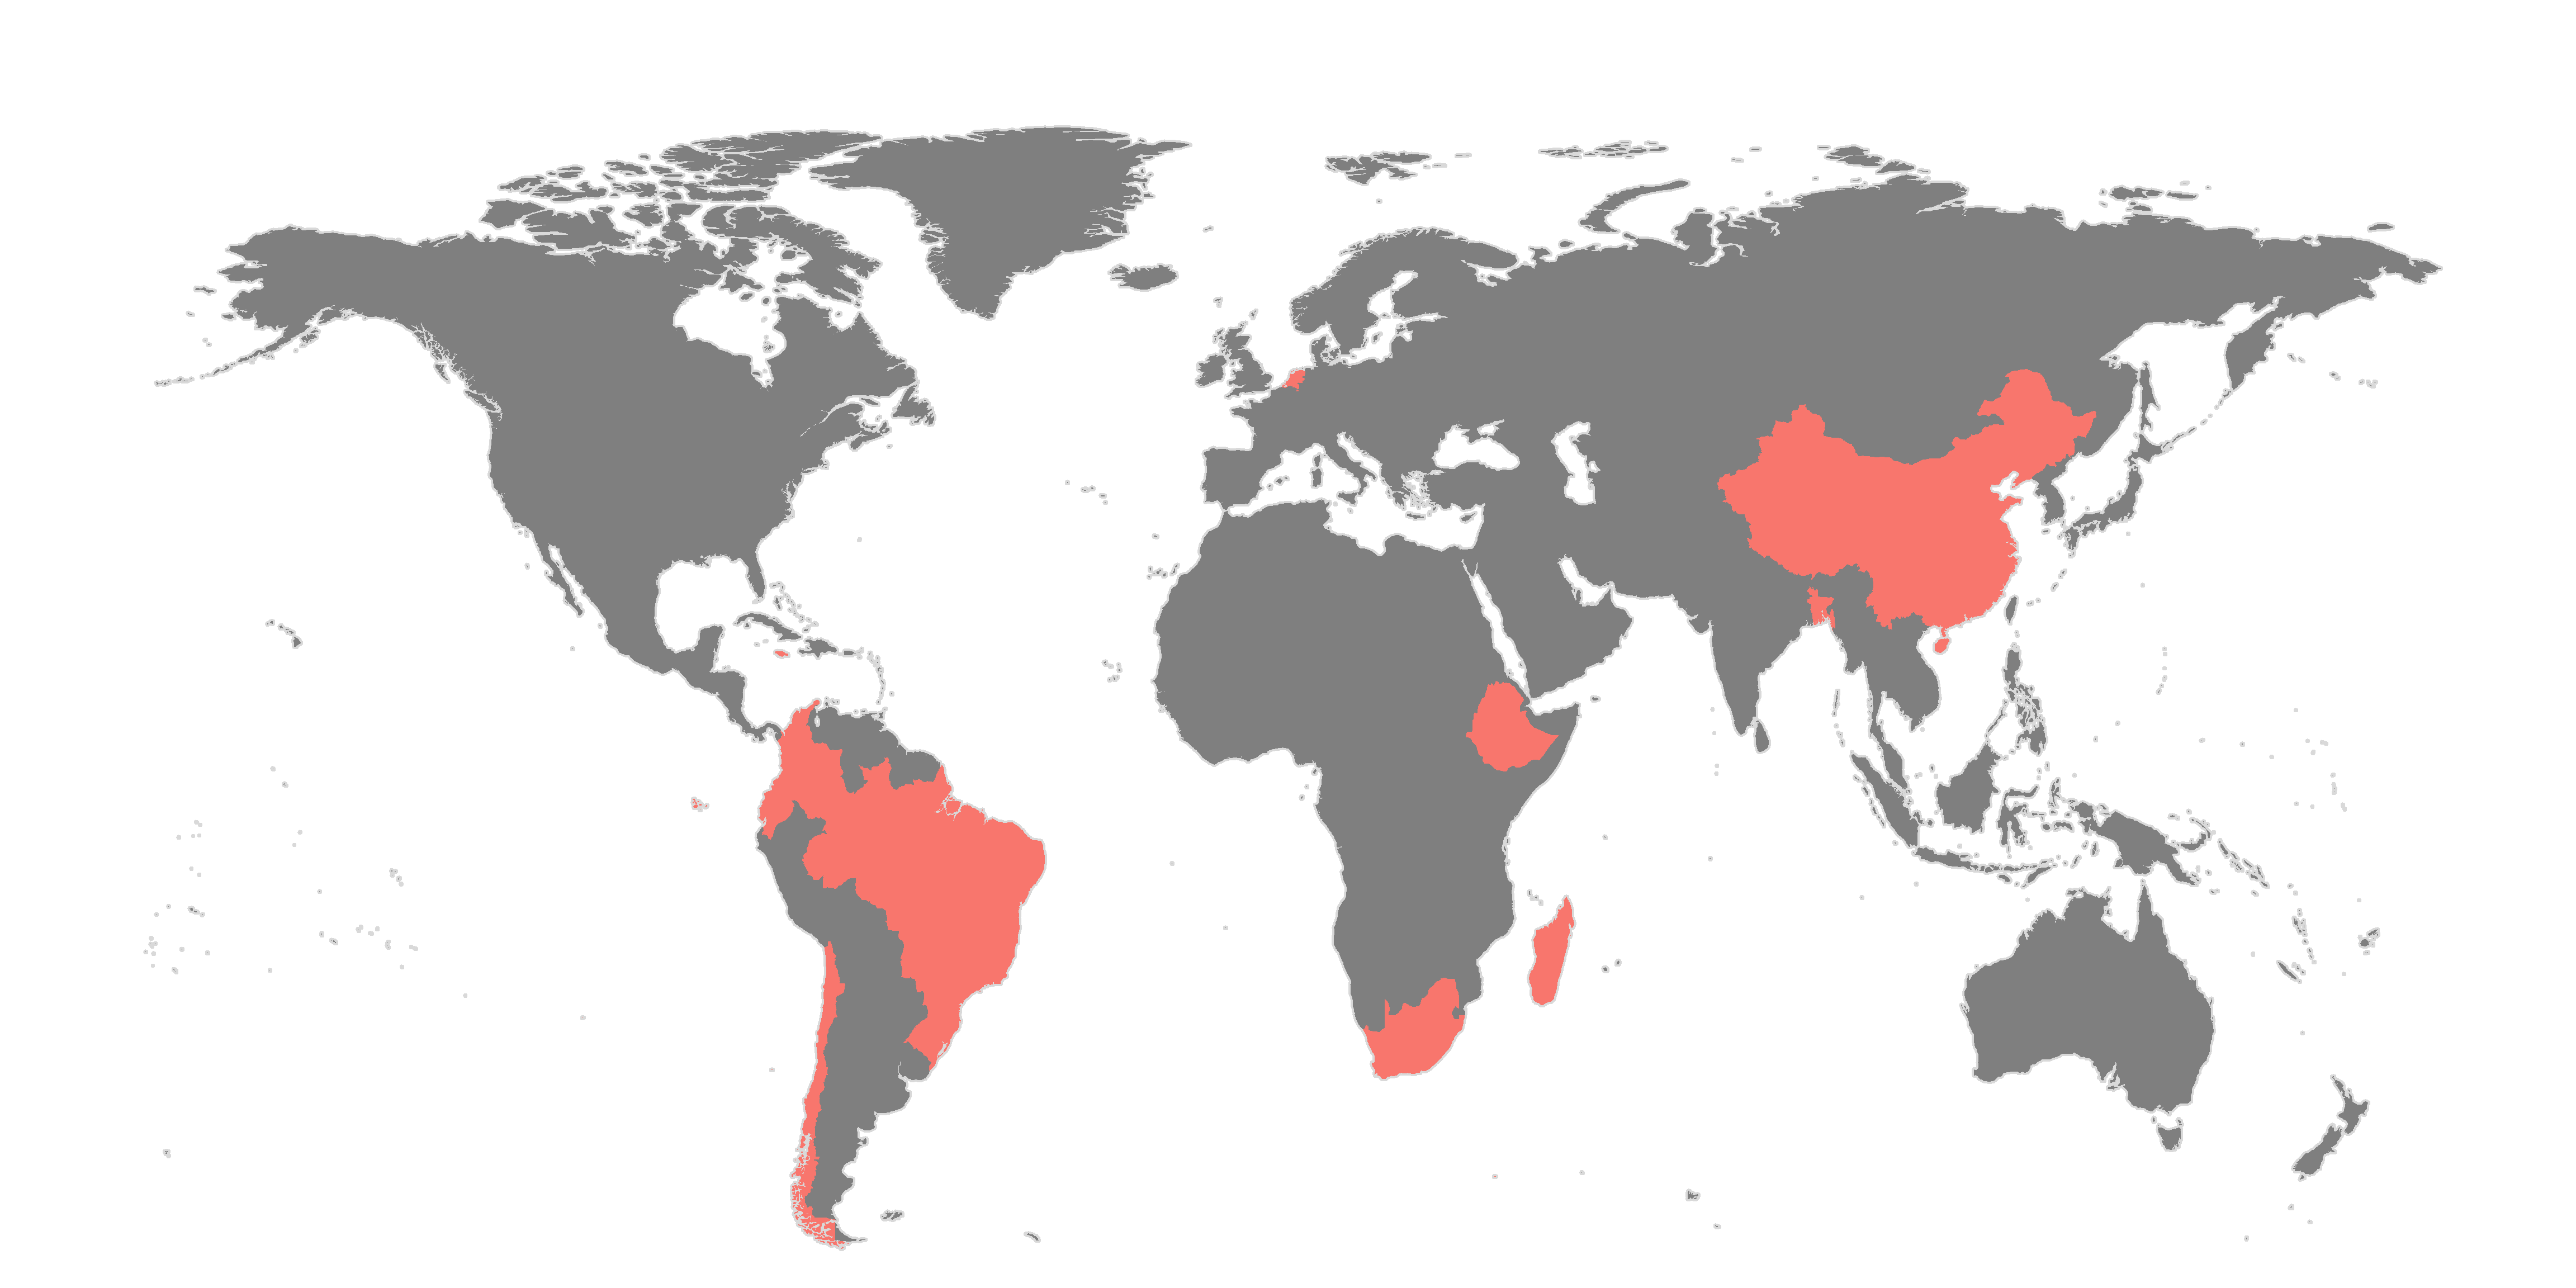
\includegraphics[width=1\linewidth]{dbook2_files/figure-latex/worldmap-1} 

}

\caption{Coverage of countries included in the study.}\label{fig:worldmap}
\end{figure}



The GCDG data comprises of birth cohorts, impact evaluation studies and instrument evaluation studies. Table \ref{tab:cohorts} displays a brief overview of the instruments used in each sub-study.

\begin{longtable}[]{@{}lllllllllll@{}}
\caption{\label{tab:cohorts} Overview of instruments administered in the cohorts.}\tabularnewline
\toprule
Cohort & \texttt{by} & \texttt{den} & \texttt{gri} & \texttt{bat} & \texttt{vin} & \texttt{ddi} & \texttt{bar} & \texttt{tep} & \texttt{aqi} & \texttt{sbi}\tabularnewline
\midrule
\endfirsthead
\toprule
Cohort & \texttt{by} & \texttt{den} & \texttt{gri} & \texttt{bat} & \texttt{vin} & \texttt{ddi} & \texttt{bar} & \texttt{tep} & \texttt{aqi} & \texttt{sbi}\tabularnewline
\midrule
\endhead
Bangladesh & x & & & & & & & & &\tabularnewline
Brazil 1 & & x & & & & & & & &\tabularnewline
Brazil 2 & & & & x & & & & & &\tabularnewline
Chile 1 & x & & & & & & & & &\tabularnewline
Chile 2 & & & & x & & & & x & &\tabularnewline
China & x & & & & & & & & &\tabularnewline
Colombia 1 & x & & & & & & & & &\tabularnewline
Colombia 2 & x & x & & x & & & & & x &\tabularnewline
Ecuador & & & & & & & x & & &\tabularnewline
Ethiopia & x & & & & & & & & &\tabularnewline
Jamaica 1 & & & x & & & & & & &\tabularnewline
Jamaica 2 & & & x & & & & & & &\tabularnewline
Madagascar & & & & & & & & & & x\tabularnewline
Netherlands1 & & & & & & x & & & &\tabularnewline
Netherlands2 & & & & & & x & & & &\tabularnewline
South Africa & x & & x & & x & & & & &\tabularnewline
\bottomrule
\end{longtable}

\hypertarget{sec:cohorts}{%
\section{Cohort descriptions}\label{sec:cohorts}}

The cohorts have different designs, age ranges and assessment instruments. Figure \ref{fig:design} displays the age range of developmental assessments per cohort, coloured according to the instruments.

\begin{figure}

{\centering 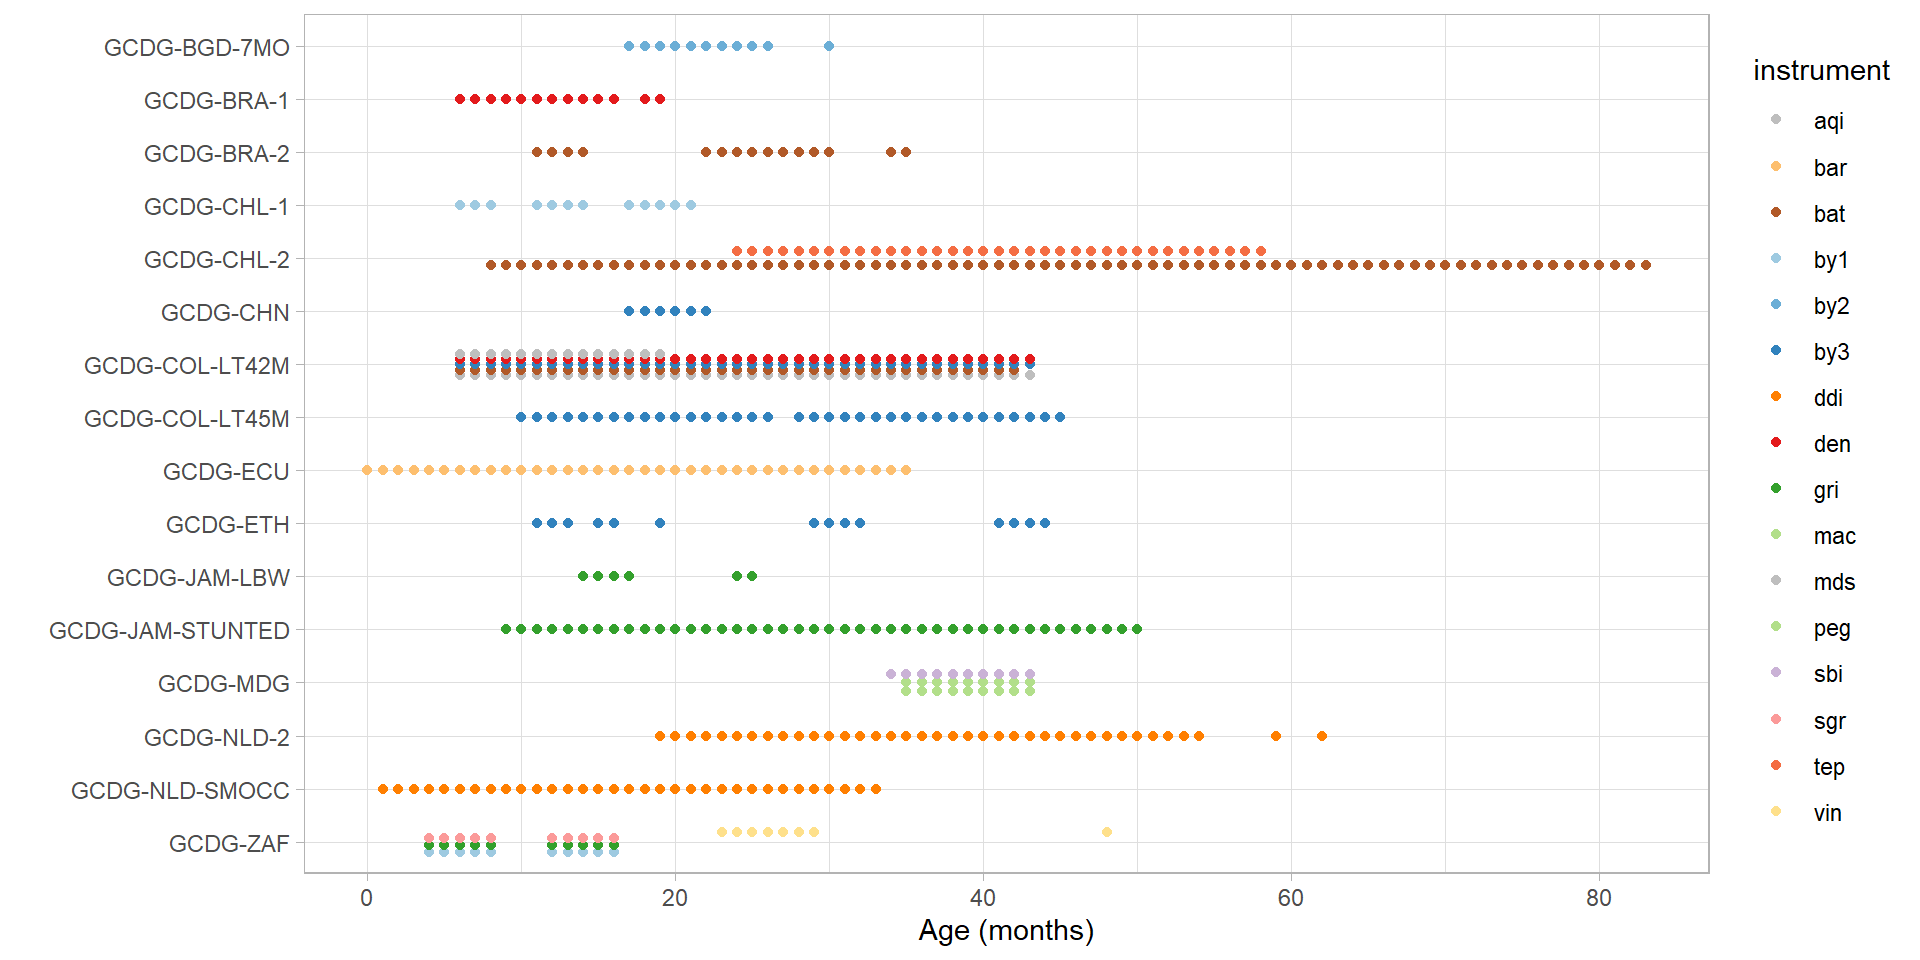
\includegraphics[width=1\linewidth]{dbook2_files/figure-latex/design-1} 

}

\caption{Age range and assessment instrument of included data for each GCDG cohort}\label{fig:design}
\end{figure}



A brief description of each cohort follows:

The \textbf{Bangladesh} study (GCDG-BGD-7MO) was an impact evaluation study including 1862 children around the age of 18 months. The Bayley Scale for Infant and Toddler Development-II (\texttt{by2}) was administered and long-term follow-up data were available for the Wechsler Preschool and Primary Scale of Intelligence (WPPSI) at 5 years (\protect\hyperlink{ref-Tofail2008}{Tofail et al. 2008}).

The \textbf{Brazil 1} study (GCDG-BRA-1) was a birth-cohort with 3 measurement moments: 644 children at 3 months, 1412 children at 6 months and 1362 children at 12 months. The investigators administered the Denver Developmental Screening Test-II (\texttt{den}) in each round. Long-term follow-up data were available for the Wechsler Adult Intelligence Scale (WAIS) at 18 years (\protect\hyperlink{ref-Victora2006}{Victora et al. 2006}).

The \textbf{Brazil 2} study (GCDG-BRA-2) was a birth-cohort with measurements of 3907 children at 12 months and 3869 children at 24 months. Both occasions collected data on the Battelle Development Inventory (\texttt{bat}) (\protect\hyperlink{ref-Moura2010}{Moura et al. 2010}).

The \textbf{Chile 1} study (GCDG-CHL-1) was an impact evaluation study of 128 children assessed at 6 months, 1732 children at 12 months and 279 at 18 months. The \texttt{by1} was administered at each of the three waves. Long-term follow-up data were available for the WPPSI at 5-6 years (\protect\hyperlink{ref-Lozoff2003}{Lozoff et al. 2003}).

The \textbf{Chile 2} study (GCDG-CHL-2) consists of a birth-cohort of 4869 children. The investigators measured child development by the Battelle Developmental Inventory (\texttt{bat}) at 7-23 months. A total of 9201 children aged 24-58 responded to the Test de Desarrollo Psicomotor (\texttt{tep}) at 24-58 months. For the latter group, follow-up data were available for the Peabody Picture Vocabulary Test (PPVT) at 5-6 years (\protect\hyperlink{ref-conteras2015}{Conteras and González 2015}).

The \textbf{China} study (GCDG-CHN) was an impact evaluation study that contained 990 children assessed with the by3 at 18 months (\protect\hyperlink{ref-Lozoff2016}{Lozoff et al. 2016}).

The \textbf{Colombia 1} study (GCDG-COL-LT45M) was an impact evaluation study that comprised two waves. Wave 1 contained 704 children at 12-24 months and wave 2 631 children at 24-41 months. The \texttt{by3} was administered at each wave. Long-term follow-up data were available for PPVT at 4-6 years (\protect\hyperlink{ref-Attanasio2014}{Attanasio et al. 2014}).

The \textbf{Colombia 2} study (GCDG-COL-LT42M) was an instrument validation study where all 1311 children aged 6-42 months were measured the \texttt{by3}. Also, there are data for a subgroup of 658 children on \texttt{den,} the Ages and Stages Questionnaire (\texttt{aqi}), and the \texttt{bat} screener. Long-term follow-up data were available for the Fifth Wechsler Intelligence Scale for Children (WISC-V) and the PPVT (\protect\hyperlink{ref-Rubio-Codina2016}{Rubio-Codina et al. 2016}).

An impact evaluation study
The \textbf{Jamaica 1} study (GCDG-JAM-LBW) was an impact evaluation study that collected data on the Griffiths Mental Development Scales (\texttt{gri}) for 225 children aged 15 months (first wave), and 218 children of aged 24 months (second wave). Long-term follow-up data were available for WPPSI and PPVT at 6 years (\protect\hyperlink{ref-Walker2004}{Walker et al. 2004}).

The \textbf{Jamaica 2} study (GCDG-JAM-STUNTED) was an impact evaluation study with data on the \texttt{gri} for 159 children at 9-24 months, 21-36 months, and at 33-48 months. Long-term follow-up data were available for \texttt{sbi}, Raven's Coloured Progressive Matrices (Ravens), and PPVT at 7-8 years and the WAIS at 17-18 years (\protect\hyperlink{ref-Grantham-McGregor1991}{Grantham-McGregor et al. 1991}).

The \textbf{Madagascar} study (GCDG-MDG) was an impact evaluation study that used the \texttt{sbi} for 205 children aged 34-42 months. Long-term follow-up data were available for \texttt{sbi} and PPVT at 7-11 years (\protect\hyperlink{ref-Fernald2011}{Lia C. H. Fernald et al. 2011}).

The \textbf{Netherlands 1} study (GCDG-NLD-SMOCC) was an instrument validation study with a total of 9 waves. At each wave the Dutch Developmental instrument (\texttt{ddi}) (In the Netherlands known as Van Wiechenschema) was administered. The first wave included 1985 children at 1 month, wave 2 1807 children at 2 months, wave 3 1963 children at 3 months, wave 4 1919 children at 6 months, wave 5 1881 children at 9 months, wave 6 1802 children at 12 months, wave 7 1776 children at 15 months, wave 8 1787 children at 18 months, and wave 9 1815 children at 24 months (\protect\hyperlink{ref-herngreen1992}{Herngreen et al. 1992}).

The \textbf{Netherlands 2} study (GCDG-NLD-2) was an instrument validation study with a total of five waves. This study resembles GCDG-NLD-SMOCC but for older children. Wave 1 included 1016 children at 24 months, wave 2 995 children at 30 months, wave 3 1592 children at 36 months, wave 4 1592 children at 42 months, and wave 5 1024 children at 48 months (\protect\hyperlink{ref-doove2010}{Doove 2010}).

The \textbf{South Africa} study (GCDG-ZAF) was a birth cohort with four waves. The first wave included 485 children and second wave 275 children, who were assessed at 6 and 12 months, respectively, with the \texttt{by1} and the \texttt{gri}. The third wave included 1802 children and the fourth wave 1614 children, assessed at 24 and 48 months, respectively, with the Vineland Social Maturity Scale (\texttt{vin}) (\protect\hyperlink{ref-Richter2007}{Richter et al. 2007}).

\hypertarget{sec:instruments}{%
\section{Instruments}\label{sec:instruments}}

The \textbf{Bayley Scales for Infant and Toddler Development (\texttt{by1},\texttt{by2}, \texttt{by3})} aim to assess infants and toddlers, aged 1-42 months. The current version is the \texttt{by3}, but some GCDG cohorts used earlier versions (i.e.~\texttt{by1} and \texttt{by2}) (\protect\hyperlink{ref-bayley1969}{Bayley 1969})(\protect\hyperlink{ref-bayley1993}{Bayley 1993})(\protect\hyperlink{ref-bayley2006}{Bayley 2006}). The 326 items of the \texttt{by3} measure three domains: Cognitive items, Motor items (with fine and gross motor items), and Language items (with expressive and receptive items). The \texttt{by2} contains 277 items and has two additional subscales: Social-Emotional and Adaptive Behavior. by1 contains 229 items.

The \textbf{Denver Developmental Screening Test (\texttt{den})} is aimed to identify developmental problems in children up to age six. The 125 dichotomous test items are distributed over the age range from birth to six years. The Denver covers four domains: personal-social, fine motor and adaptive, language, and gross motor. The test items are all directly observed by an examiner and are not dependent on parent report (\protect\hyperlink{ref-frankenburg1992}{Frankenburg et al. 1992}) (\protect\hyperlink{ref-frankenburg1990}{Frankenburg et al. 1990}).

The \textbf{Griffiths Mental Development Scales (\texttt{gri})} measure the rate of development in infants and young children in six developmental areas: locomotor, personal-social, hearing and language, eye and hand coordination, performance and practical reasoning (\protect\hyperlink{ref-griffiths1967}{Griffiths 1967}).

The \textbf{Battelle Developmental Inventory (\texttt{bat})} measures key developmental skills in children from birth to 7 years, 11 months. The instrument contains 450 items distributed over five domains: adaptive, personal-social, communication, motor, and cognitive (\protect\hyperlink{ref-newborg2005}{Newborg 2005}).

The \textbf{Vineland Social Maturity Scale (\texttt{vin})} is a test to assess social competence. The instrument contains eight subscales that measure communication skills, general self-help ability, locomotion skills, occupation skills, self-direction, self-help eating, self-help dressing and socialisation skills (\protect\hyperlink{ref-doll1953}{Doll 1953}).

The \textbf{Dutch Developmental Instrument (\texttt{ddi})} measures early child development during the ages 0-4 years. The instrument consists of 75 milestones spread over three domains: fine motor, adaptive, personal and social behaviour; communication; and gross motor (\protect\hyperlink{ref-schlesinger1981}{Schlesinger-Was 1981}).

The \textbf{Barrera Moncada (\texttt{bar})} is a Spanish instrument that measures the growth and psychological development of children (\protect\hyperlink{ref-barrera1981}{Barrera Moncada 1981}).

The \textbf{Test de Desarrollo Psicomotor (\texttt{tep})} is an instrument to evaluate toddlers aged 2 to 5 years on their development. The items come from three sub-tests: 16 items assess coordination; 24 items measure language skills and 12 items tap into motor skills (\protect\hyperlink{ref-haeussler1999}{Haeussler and Marchant 1999}).

The \textbf{Ages and Stages Questionnaire (\texttt{aqi})} measures developmental progress in children aged 2 mo -- 5.5 yrs. The instrument distinguishes development in five areas: personal-social, gross motor, fine motor, problem solving, and communication. The caregiver completes 30 items per age intervals and (\protect\hyperlink{ref-squires2009}{Squires and Bricker 2009}).

The \textbf{Stanford Binet Intelligence Scales (\texttt{sbi})} is a cognitive ability and intelligence test to diagnose developmental deficiencies in young children. The items divide into five subtests: fluid reasoning, knowledge, quantitative reasoning, visual-spatial processing, and working memory (\protect\hyperlink{ref-roid2003}{Roid 2003})(\protect\hyperlink{ref-hagen1986}{Hagen and Stattler 1986}).

\hypertarget{ch:comparability}{%
\chapter{Comparability}\label{ch:comparability}}

\begin{quote}
Author: Iris Eekhout, Stef van Buuren
\end{quote}

This chapter describes challenges and methodologies to harmonize child development measurements obtained by different instruments:

\begin{itemize}
\tightlist
\item
  Are instruments connected? (\ref{sec:challenge})
\item
  Bridging instruments by mapping items (\ref{sec:mapping})
\item
  Overview of promising item mappings (\ref{sec:viewmapping})
\end{itemize}

\hypertarget{sec:challenge}{%
\section{Are instruments connected?}\label{sec:challenge}}

The ultimate goal is to compare child development across populations and cultures. A complication is that measurements are made by different instruments. To do deal with this issue, we harmonize the data included in the GCDG cohorts. In particular, we process the milestone responses such that the following requirements hold:

\begin{itemize}
\tightlist
\item
  Every milestone in an instrument has a unique name and a descriptive label;
\item
  Every milestone occupies one column in the dataset;
\item
  Item scores are (re)coded as: 1 = PASS; 0 = FAIL;
\item
  Items not administered or not answered are a missing value;
\item
  Every row in the dataset corresponds to a unique cohort-child-age combination.
\end{itemize}

Cohorts and milestones need to be \emph{connected}. There are several ways to connect cohorts:

\begin{itemize}
\tightlist
\item
  Two cohorts are directly connected if they use the same instrument;
\item
  Two cohorts are indirectly connected if both connect to a third cohort that connects them.
\end{itemize}

Likewise, instruments can be connected:

\begin{itemize}
\tightlist
\item
  Two instruments are directly connected if the same cohort measures both;
\item
  Two instruments are indirectly connected if both connect to a third instrument that connects them.
\end{itemize}

\begin{table}

\caption{\label{tab:linkage}Linkage pattern indicating combinations of cohorts and instruments.}
\centering
\begin{tabular}[t]{llllllllllllllll}
\toprule
  & aqi & bar & bat & by1 & by2 & by3 & ddi & den & gri & mac & peg & sbi & sgr & tep & vin\\
\midrule
Bangladesh &  &  &  &  & X &  &  &  &  &  &  &  &  &  & \\
Brazil 1 &  &  &  &  &  &  &  & X &  &  &  &  &  &  & \\
Brazil 2 &  &  & X &  &  &  &  &  &  &  &  &  &  &  & \\
Chile 1 &  &  &  & X &  &  &  &  &  &  &  &  &  &  & \\
Chile 2 &  &  & X &  &  &  &  &  &  &  &  &  &  & X & \\
\addlinespace
China &  &  &  &  &  & X &  &  &  &  &  &  &  &  & \\
Colombia 1 &  &  &  &  &  & X &  &  &  &  &  &  &  &  & \\
Colombia 2 & X &  & X &  &  & X &  & X &  &  &  &  &  &  & \\
Ecuador &  & X &  &  &  &  &  &  &  &  &  &  &  &  & \\
Ethiopia &  &  &  &  &  & X &  &  &  &  &  &  &  &  & \\
\addlinespace
Jamaica 1 &  &  &  &  &  &  &  &  & X &  &  &  &  &  & \\
Jamaica 2 &  &  &  &  &  &  &  &  & X &  &  &  &  &  & \\
Madagascar &  &  &  &  &  &  &  &  &  & X & X & X &  &  & \\
Netherlands1 &  &  &  &  &  &  & X &  &  &  &  &  &  &  & \\
Netherlands2 &  &  &  &  &  &  & X &  &  &  &  &  &  &  & \\
\addlinespace
South Africa &  &  &  &  & X &  &  &  & X &  &  &  & X &  & X\\
\bottomrule
\end{tabular}
\end{table}

~

An \texttt{X} in Table \ref{tab:linkage} identifies which cohorts use which instruments. The linkage table shows that studies from China, Colombia, and Ethiopia are directly connected (by \texttt{by3}). Brazil 1 indirectly connects to these studies through \texttt{den}. Some cohorts (e.g., Chile 1 and Ecuador) do not link to any other study. Likewise, we might say that \texttt{aqi}, \texttt{bat}, \texttt{by3}, and \texttt{den} are directly connected. Note that no indirect connections exist to this instrument group.

Table \ref{tab:linkage} is a somewhat simplified version of the linkage pattern. As we saw in section \ref{sec:cohorts}, there are substantial age differences between the cohorts. The linked \href{https://tnochildhealthstatistics.shinyapps.io/GCDG_instrument_linkage/}{instrument linkage table} shows the counts of the number of registered scores per age group. What appears in Table \ref{tab:linkage} as one test may comprise of two disjoint subsets, and hence some cohorts may not be connected after all.

Connectedness is a necessary - though not sufficient - requirement for parameter identification. If two cohorts are not connected, we cannot distinguish between the following two alternative explanations:

\begin{itemize}
\tightlist
\item
  Any differences between studies can be attributed to the ability of the children;
\item
  Any differences between studies can be attributed to the difficulties of the instruments.
\end{itemize}

The data do not contain the necessary information to discriminate between these two explanations. Since many cohorts in Table \ref{tab:linkage} are unconnected, it seems that we are stuck.

The next section suggests a way out of the dilemma.

\hypertarget{sec:mapping}{%
\section{Bridging instruments by mapping items}\label{sec:mapping}}

Many instruments for measuring child development have appeared since the works of \protect\hyperlink{ref-shirley1933}{Shirley} (\protect\hyperlink{ref-shirley1933}{1933}) and \protect\hyperlink{ref-gesell1943}{Gesell} (\protect\hyperlink{ref-gesell1943}{1943}). It is no surprise that their contents show substantial overlap. All tools assess events like starting to see, hear, smile, fetch, crawl, walk, speak, and think. We will exploit this overlap to bridge different instruments. For example, Table \ref{tab:example2words} displays the labels of milestones from six instruments. All items probe the ability of the child to formulate ``sentences'' of two words.

\begin{table}

\caption{\label{tab:example2words}Example of similar items from different instruments.}
\centering
\begin{tabular}[t]{>{}ll}
\toprule
Item & Label\\
\midrule
\ttfamily{by1mdd136} & sentence of 2 words\\
\ttfamily{by2mdd114} & Uses a two-word utterance\\
\ttfamily{ddicmm041} & Says sentences with 2 words\\
\ttfamily{denlgd019} & Combine Words\\
\ttfamily{grihsd217} & Uses word combinations\\
\addlinespace
\ttfamily{vinxxc016} & use a short sentence\\
\bottomrule
\end{tabular}
\end{table}

~

The idea is to check whether these milestones measure development in the same way. If this is found to be true, then we may formally restrict the difficulty levels of these milestones to be identical. This restriction provides a formal bridge between the instruments. We repeat the process for all groups of similar-looking items.

A first step in the bridging process is to group items from different instruments by similarity. As the \texttt{by3} is relatively long and is the most often used instrument, it provides a convenient starting point. Subject matter experts experienced in child development mapped items from other tools to \texttt{by3} items. These experts evaluated the similarity of wordings and descriptions in reference manuals. Also, they mapped same-skill items across other instruments into groups if these did not map onto \texttt{by3} items.

\begin{figure}

{\centering 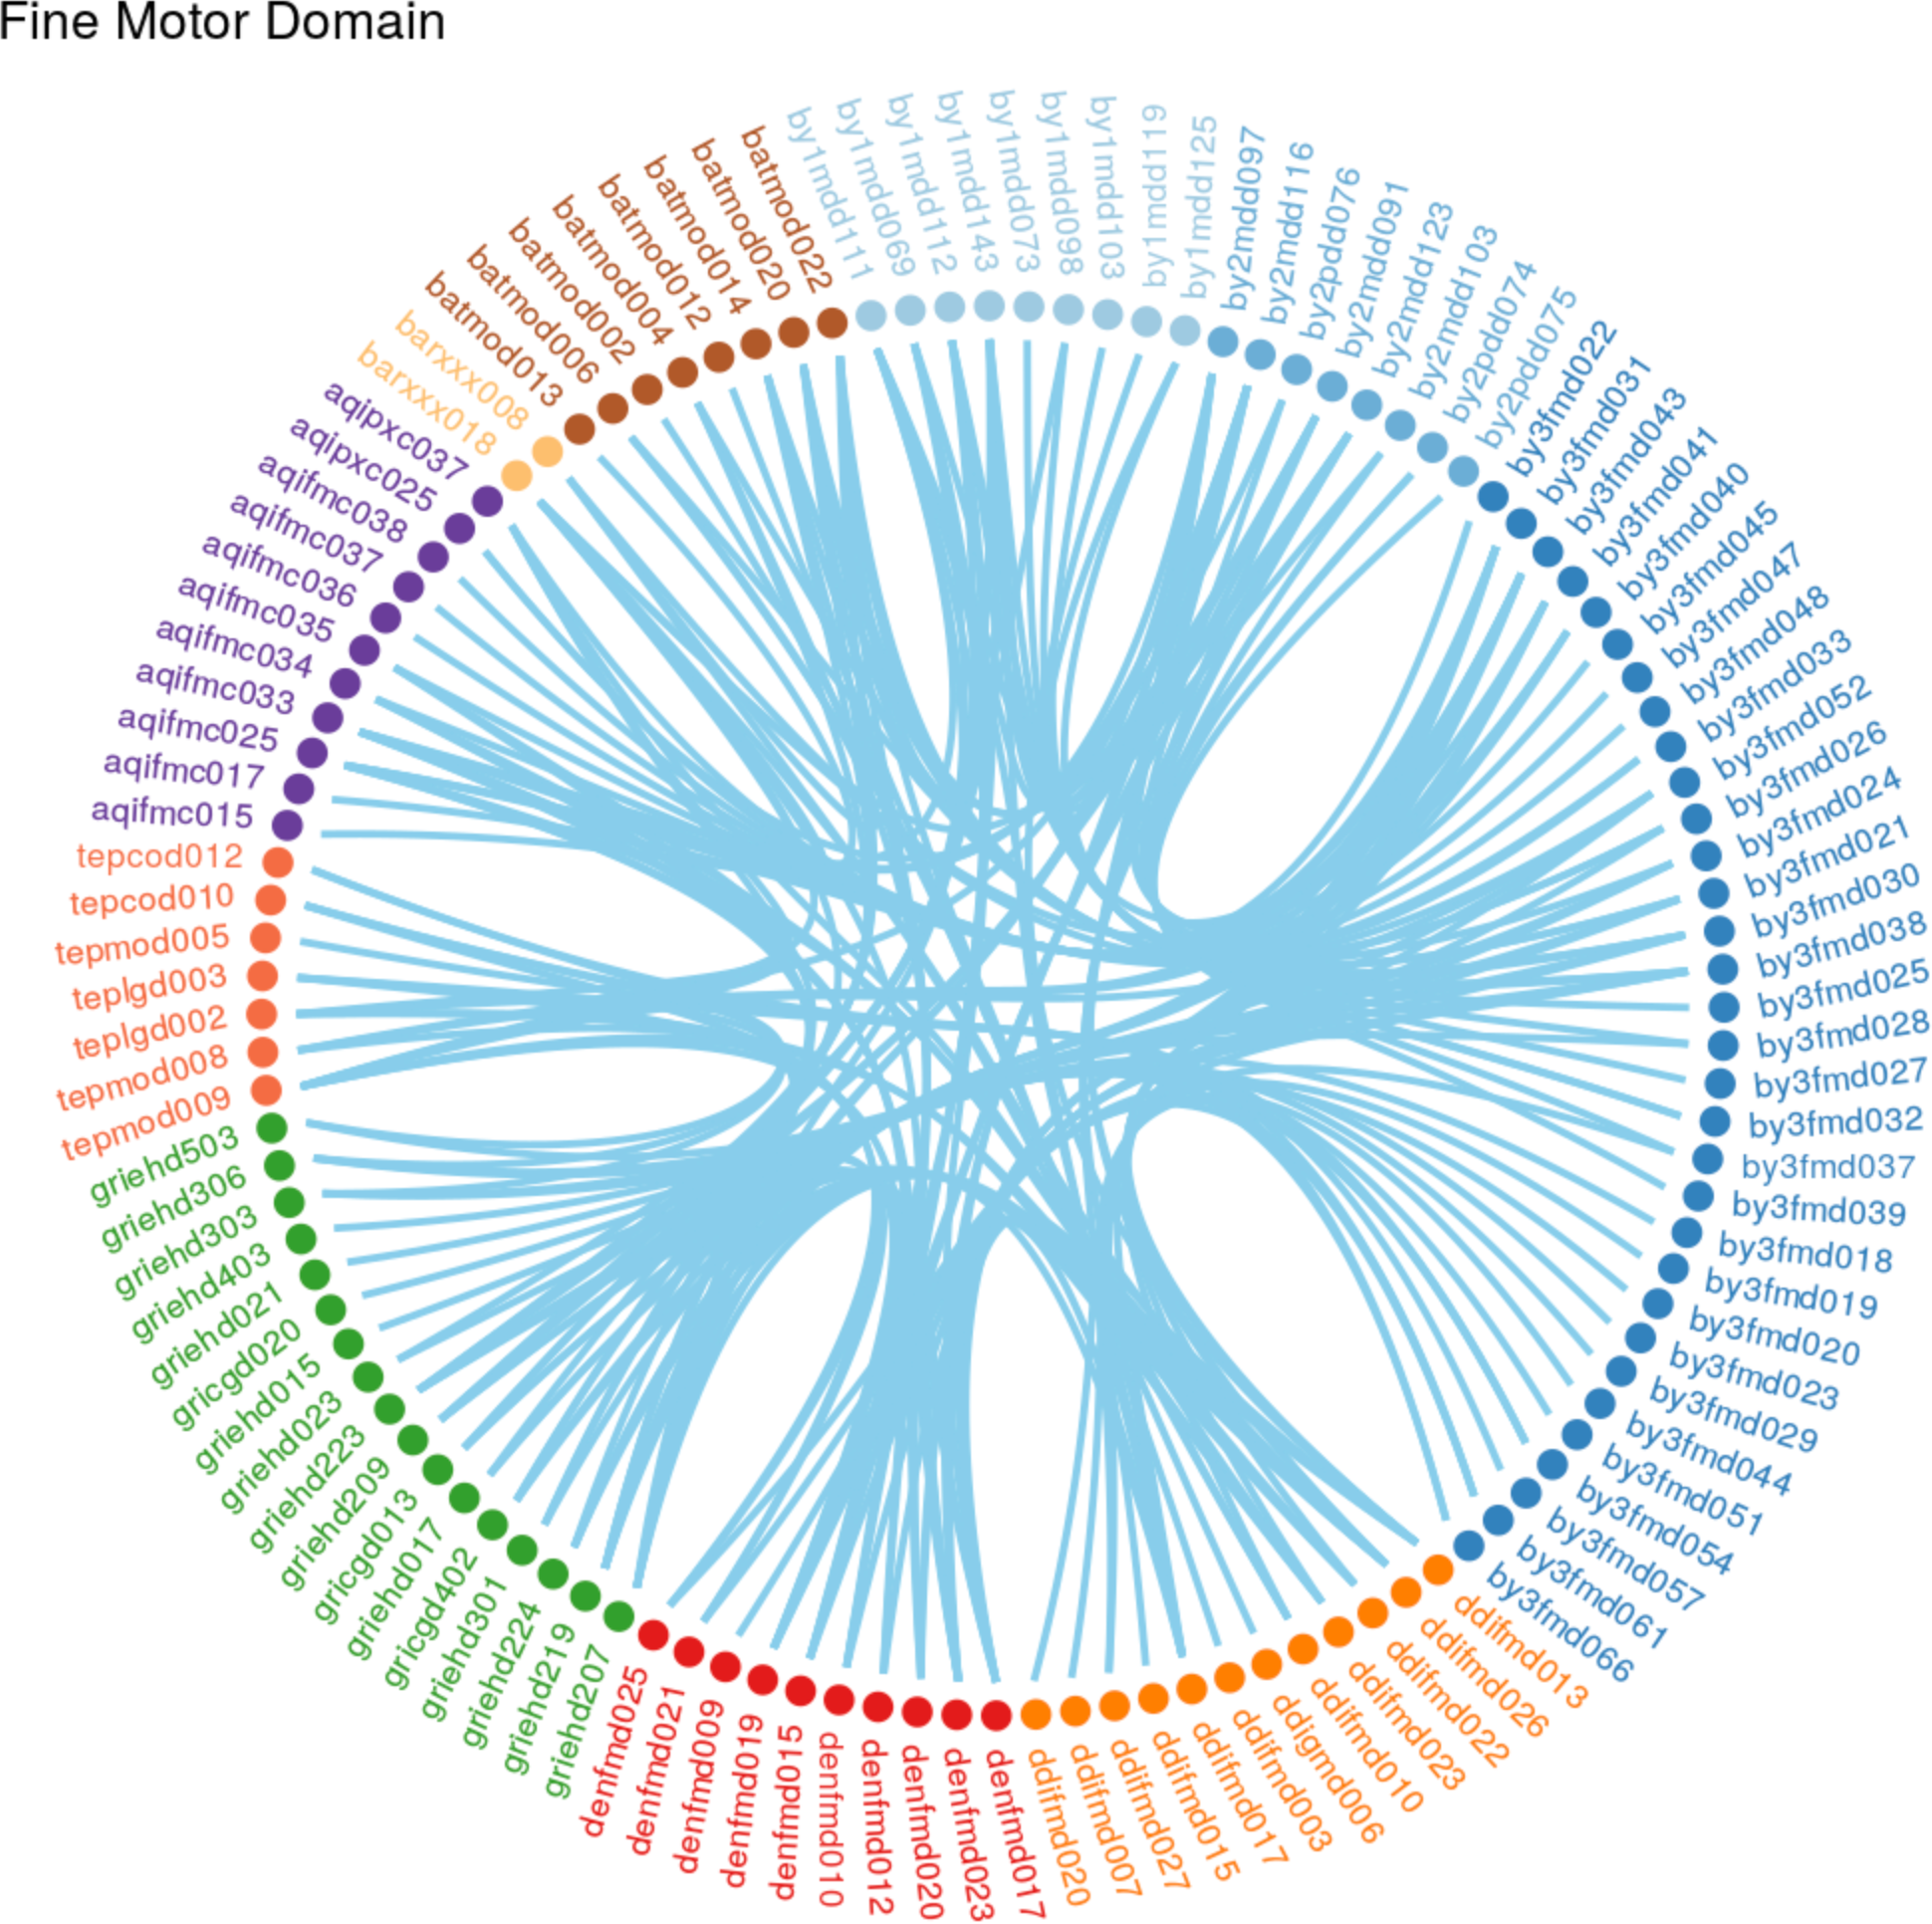
\includegraphics[width=1\linewidth]{fig/ring} 

}

\caption{Connections between the instruments via mapped item groups by domain (\url{https://tnochildhealthstatistics.shinyapps.io/GCDG_mapping/}).}\label{fig:mappingshiny}
\end{figure}



Figure \ref{fig:mappingshiny} connects similar items and hence visualises connections between instruments. Items are displayed in the wheel, coloured by instrument. We organised item mappings into five domains: fine motor (FM), gross motor (GM), cognitive (COG), receptive (REC), and expressive (EXP). The \texttt{Prev} and \texttt{Next} buttons allow us to visit other domains.

\hypertarget{sec:viewmapping}{%
\section{Age profile of item mappings}\label{sec:viewmapping}}

Another way to explore the similarity of milestones from different instruments is to plot the probability of passing by age. Figure \ref{fig:poteq} shows two examples. The first graph presents the age curves of a group of four cognitive items for assessing the ability to put a cube or block in a cup or box. The milestones are administered in different studies and seem to work similarly. The second plot shows a similar graph for items that assess the ability to build a tower of six cubes or blocks. These milestones have similar age patterns as well.

\begin{figure}

{\centering 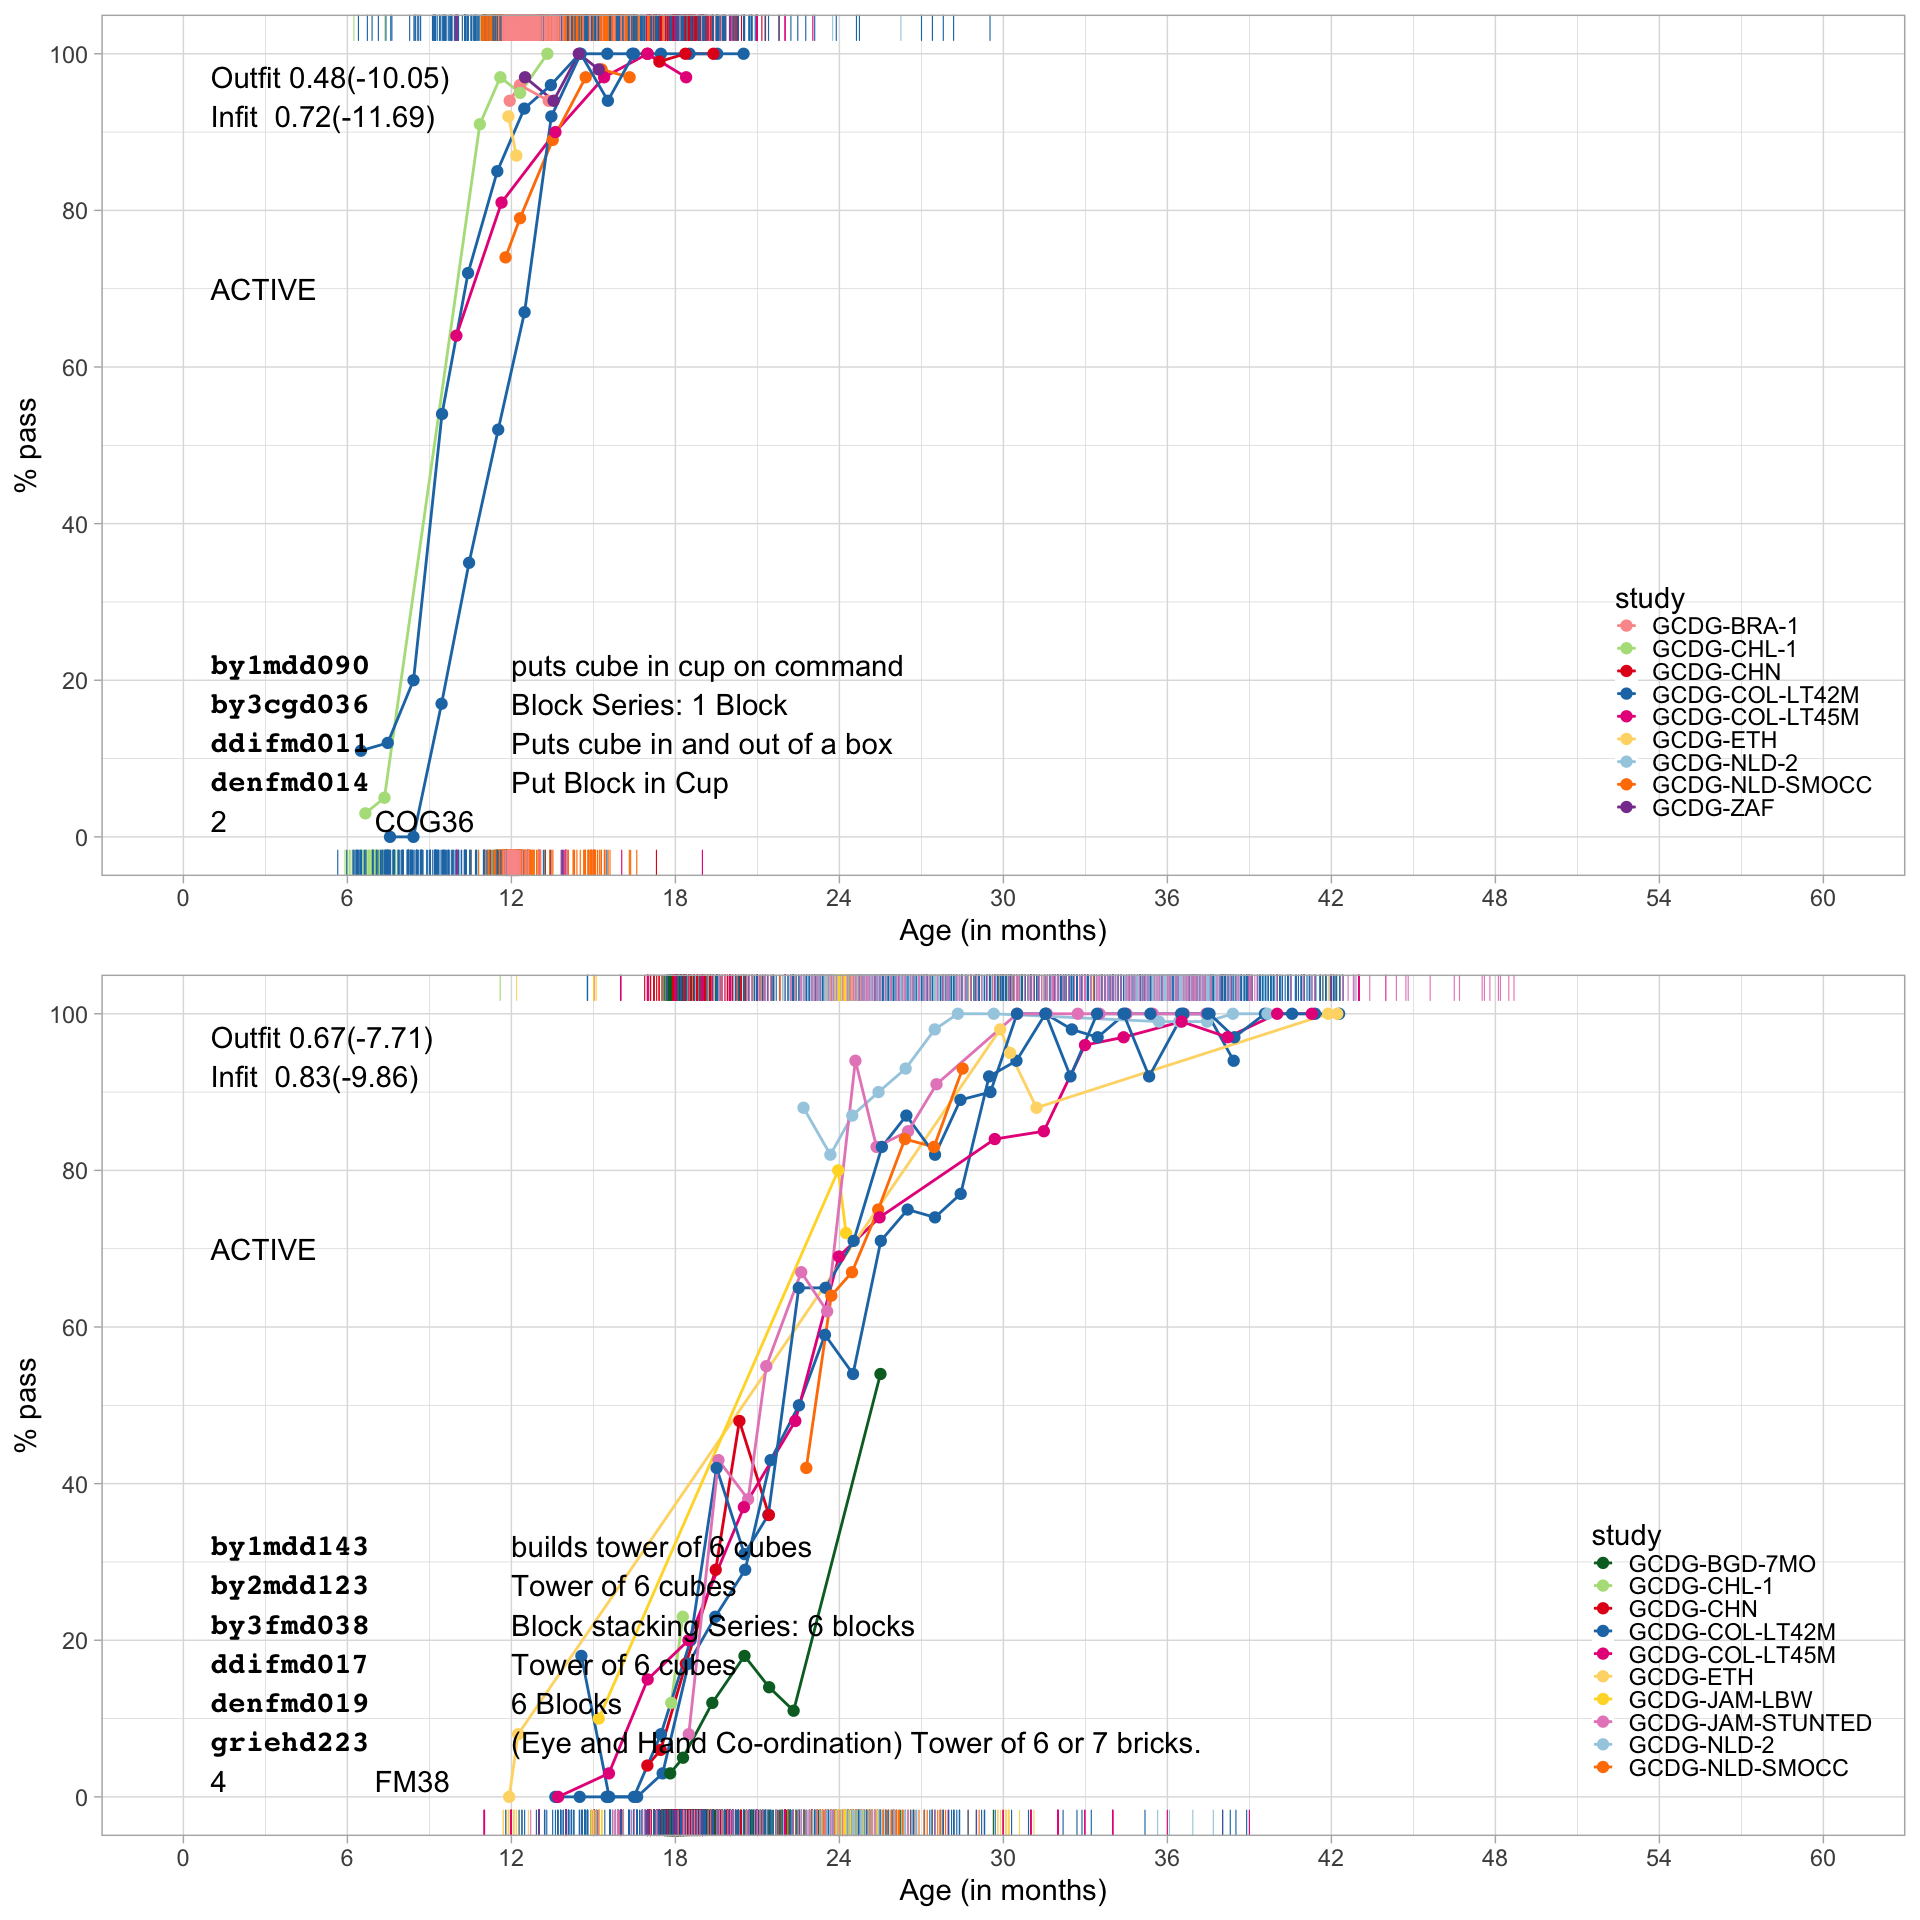
\includegraphics[width=1\linewidth]{dbook2_files/figure-latex/poteq-1} 

}

\caption{The probability of passing by age in potential bridging items.}\label{fig:poteq}
\end{figure}



Figure \ref{fig:badeq} presents two examples of weak item mappings. Notable timing differences exist for the ``babbles'' and ``bangs'' milestones, which suggests that we should not take these as bridges.

\begin{figure}

{\centering 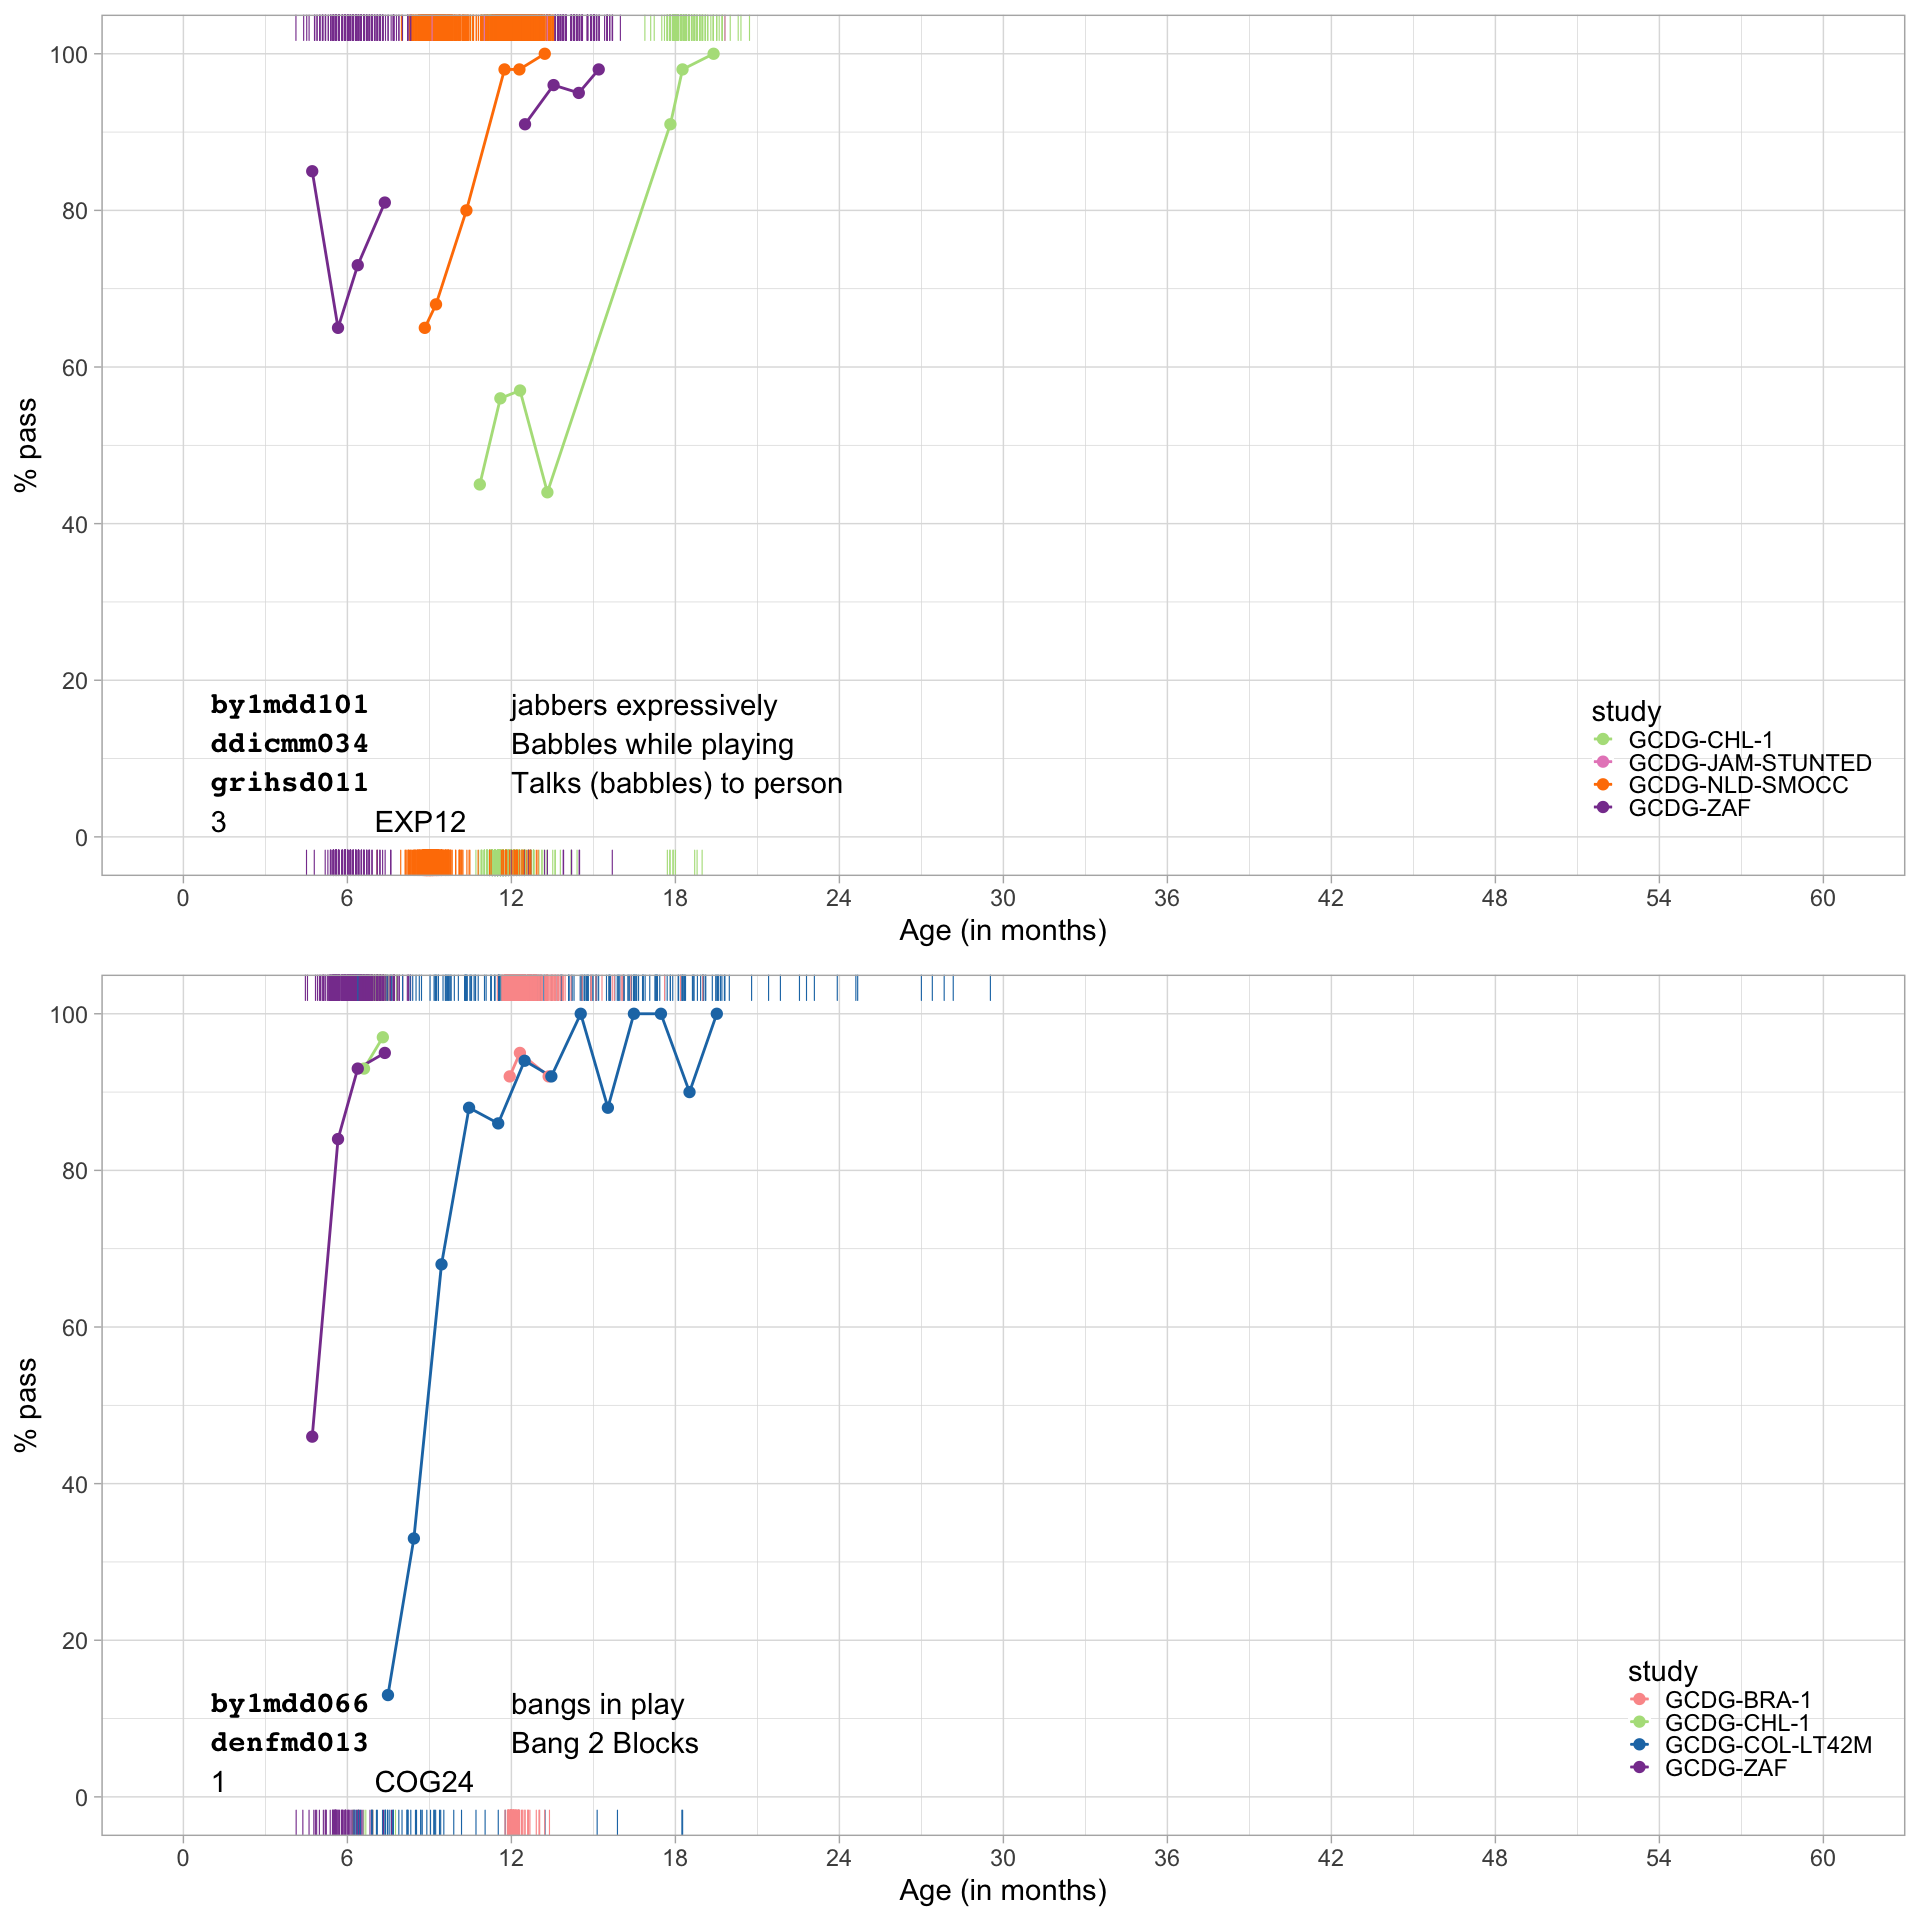
\includegraphics[width=1\linewidth]{dbook2_files/figure-latex/badeq-1} 

}

\caption{Probability to pass items for age in poor bridges.}\label{fig:badeq}
\end{figure}



While these plots are suggestive, their interpretation is surprisingly complicated. We may find that age profiles of two milestones \emph{A and B} administered in samples 1 and 2 respectively \emph{are identical} if

\begin{itemize}
\tightlist
\item
  A and B are equally difficult and samples 1 and 2 have the same maturation level;
\item
  A is more difficult than B and sample 1 is more advanced than 2.
\end{itemize}

Similarly, we may find that the age profile for \emph{A is earlier than B} if

\begin{itemize}
\tightlist
\item
  A is easier than B and if samples 1 and 2 have the same level of maturation;
\item
  A and B are equally difficult and if sample 1 is more advanced than sample 2.
\end{itemize}

Note that the age curves confound difficulty and ability, and hence cannot be used to evaluate the quality of the item map.

What we need to do is separate difficulty and ability. For this, we need a formal statistical model. The next chapter introduces the concepts required in such a model.

\hypertarget{ch:equategroups}{%
\chapter{Equate groups}\label{ch:equategroups}}

\begin{quote}
Author: Iris Eekhout, Stef van Buuren
\end{quote}

This chapter introduces the concepts and tools needed to link assessments made by different instruments administered across multiple cohorts. Our methodology introduces the idea of an equate group. Systematic application of equate groups provides a robust yet flexible methodology to link different instruments. Once the links are in place, we may combine the data to enable meta-analyses and related methods.

\begin{itemize}
\tightlist
\item
  What is an equate group? (\ref{sec:eqdef})
\item
  Concurrent calibration (\ref{sec:concurrent})
\item
  Strategy to form and test equate groups (\ref{sec:equaterules})
\item
  Statistical framework (\ref{sec:statisticalframe})
\item
  Common latent scale (\ref{sec:commonscale})
\item
  Quantifying equate fit (\ref{sec:equatefit})
\item
  Differential Item Functioning (\ref{sec:equatedif})
\end{itemize}

\hypertarget{sec:eqdef}{%
\section{What is an equate group?}\label{sec:eqdef}}

An \emph{equate group} is a set of two or more milestones that measure the same thing in (perhaps slightly) different ways. Table \ref{tab:example2words} contains an example of an equate group, containing items that measure the ability to form two-word sentences. Also, Figures \ref{fig:poteq} and \ref{fig:badeq} show examples of equate groups.

Equate groups vary in quality. We can use high-quality equate groups to link instruments by restricting the difficulty of all milestones in the equate group to be identical. Equate groups thus provide a method for bridging different tools.

\begin{figure}

{\centering 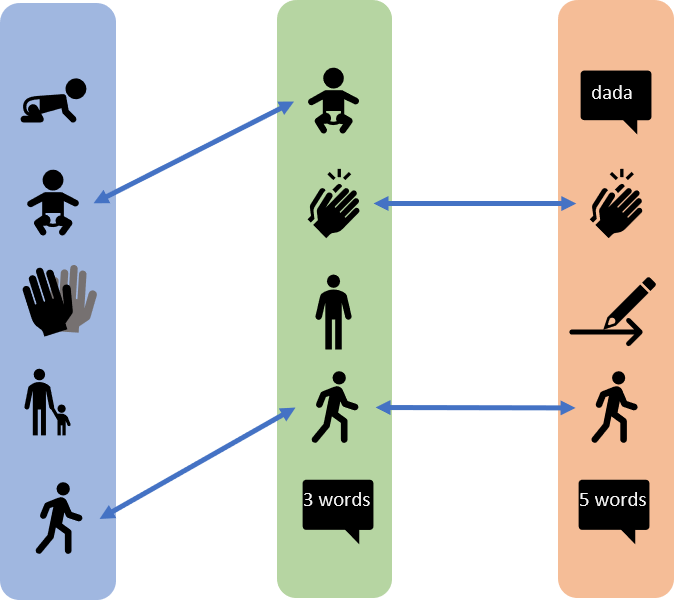
\includegraphics[width=0.75\linewidth]{fig/equate_ex} 

}

\caption{Example of three instruments that are bridged by common items in equate groups.}\label{fig:equateex}
\end{figure}



Figure \ref{fig:equateex} displays items from three different instruments with overlapping sets of milestones. The shared items make up equate groups, as presented by the arrows between them. In the example, all three instruments share one milestone (``walk alone''). The ``sitting'' and ``clap hand'' items appear in two tools. So in total, there are three equate groups.

\hypertarget{sec:concurrent}{%
\section{Concurrent calibration}\label{sec:concurrent}}

Patterns as in Figure \ref{fig:equateex} occur if we have multiple forms of the same instrument. Although in theory, there might be sequence effects, the usual working assumption is that we may ignore them. Equate groups with truly shared items that work in the same way across samples are of high quality. We may collect the responses on identical items into the same column of the data matrix. As a consequence, usual estimation methods will automatically produce one difficulty estimate for that column (i.e.~common item).

The procedure described above is known as \emph{concurrent calibration}. See \protect\hyperlink{ref-kim1998}{Kim and Cohen} (\protect\hyperlink{ref-kim1998}{1998}) for more background. The method simultaneously estimates the item parameters for all instruments. Concurrent calibration is an attractive option for various reasons:

\begin{itemize}
\tightlist
\item
  It yields a common latent scale across all instruments;
\item
  It is efficient because it calibrates all items in a single run;
\item
  It produces more stable estimates for common items in small samples.
\end{itemize}

However, concurrent calibration depends on a strict distinction between items that are indeed the same across instruments and items that differ.

In practice, strict black-white distinctions may not be possible. Items that measure the same skill may have been adapted to suit the format of the instrument (e.g.~number of response options, question formulation, and so on). Also, investigators may have altered the item to suit the local language and cultural context. Such changes may or may not affect the measurement properties. The challenge is to find out whether items measure the underlying construct in the same way.

In practice, we may need to perform concurrent calibration to multiple - perhaps slightly dissimilar - milestones. When confronted with similar - but not identical - items, our strategy is first to form provisional equate groups. We then explore, test and rearrange these equate groups, in the hope of finding enough high-quality equate groups that will bridge instruments.

\hypertarget{sec:equaterules}{%
\section{Strategy to form and test equate groups}\label{sec:equaterules}}

An equate group is a collection of items. Content matter experts may form equate groups by evaluating the contents of items and organising them into groups with similar meaning. The modelling phase takes this set of equate groups (which may be hundreds) as input. Based on the analytic result, we may activate or modify equate groups. It is useful to distinguish between \emph{active} and \emph{passive} equate groups. What do we mean by these terms?

\begin{itemize}
\tightlist
\item
  \emph{Active equate group}: The analysis treats all items within an active equate group as one super-item. The items obtain the same difficulty estimate and are assumed to yield equivalent measurements. As the items in an active equate group may originate from different instruments, such a group acts as a bridge between instruments.
\item
  \emph{Passive equate group}: Any non-active equate groups are called passive. The model does not restrict the difficulty estimates, i.e., the milestones within a passive equate group will have separate difficulty estimates.
\end{itemize}

Since active equate groups bridge different instruments, they have an essential role in the analysis. In general, we will set the status of an equate group to active \emph{only} if we believe that the milestones in that group measure the underlying construct in the same way. Note that this does not necessarily imply that all items need to be identical. In Table \ref{tab:example2words}, for example, small differences exist in item formulation. We may nevertheless believe that these are irrelevant and ignore these in practice. Reversely, there is no guarantee that the same milestone will measure child development in the same way in different samples. For example, a milestone like ``climb stairs'' could be more difficult (and more dangerous) for children who have never seen a staircase.

\begin{figure}

{\centering 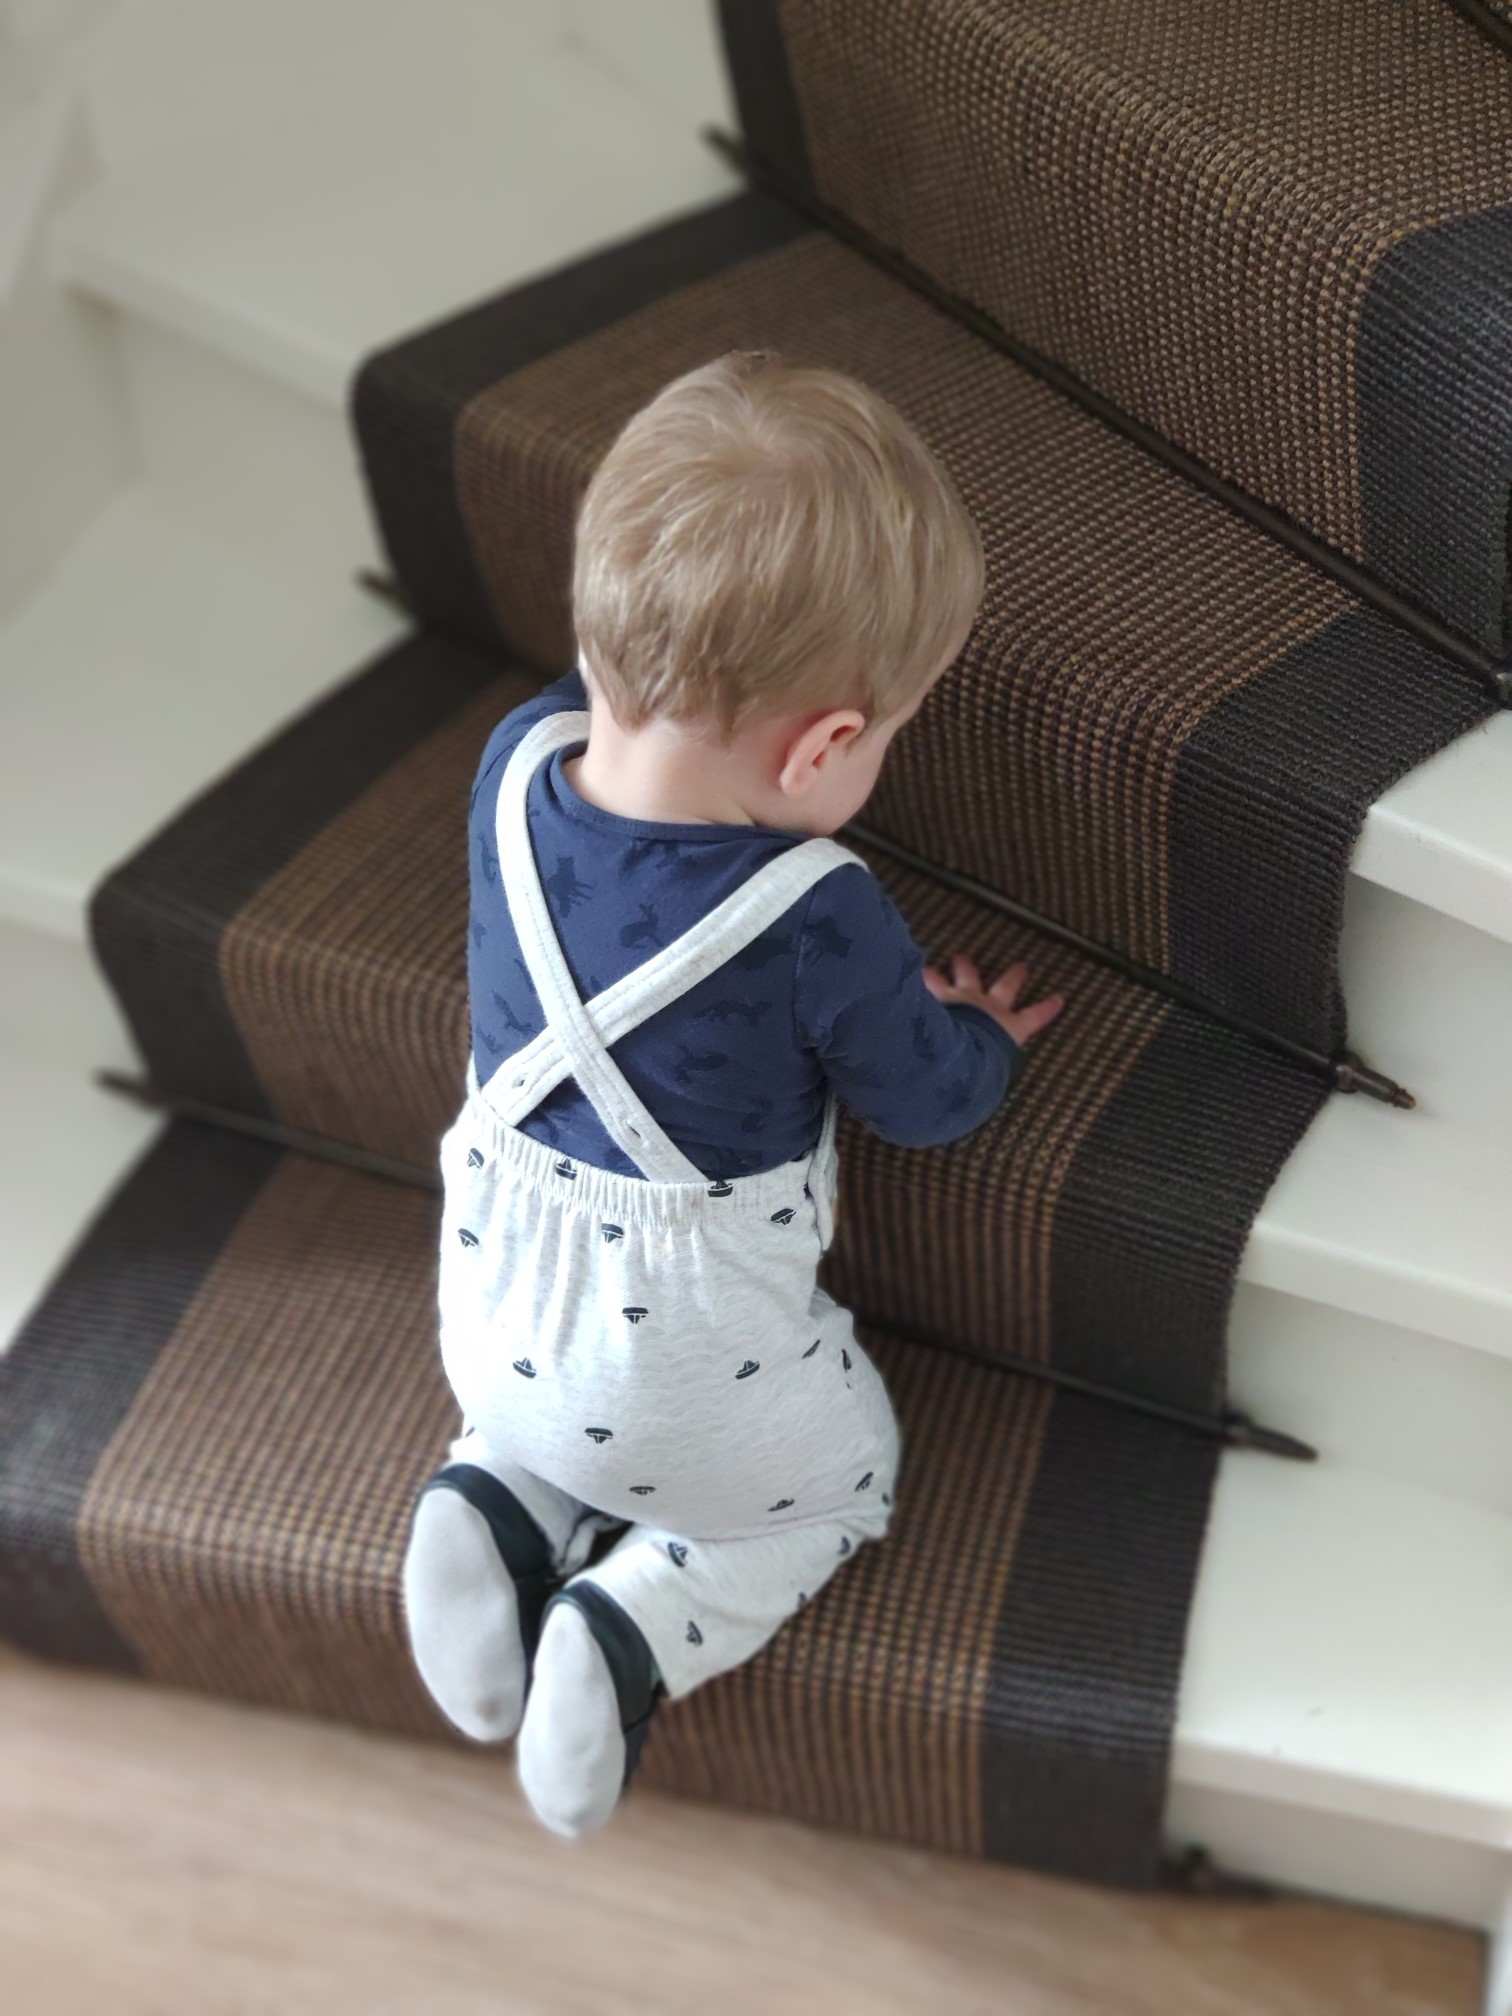
\includegraphics[width=0.5\linewidth]{fig/otis-stairs} 

}

\caption{One year old child climbs stairs.}\label{fig:stairpic}
\end{figure}



The data analysis informs decisions to activate equate groups. The following steps implement our strategy for forming and enabling equate groups:

\begin{itemize}
\tightlist
\item
  Content matter experts compare milestones from different instruments and sort similar milestones into equate groups. It may be convenient to select one instrument as a starting point, and map items from others to that (see section \ref{sec:mapping});
\item
  Visualise age profiles of mapped items (see section \ref{sec:viewmapping}). Verify the plausibility of potential matches through similar age profiles. Break up mappings for which age profiles appear implausible. This step requires both statistical and subject matter expertise;
\item
  Fit the model to the data using a subset of equate groups as active. Review the quality of the solution and optimise the quality of the links between tools by editing the equate group structure. The technical details of this model are explained in section \ref{sec:statisticalframe}. Refit the model until (1) active equate groups link all cohorts and instruments, (2) active equate groups are distributed over the full-scale range (rather than being centred at one point);
\item
  Assess the quality of equate groups by the infit and outfit (see section \ref{sec:equatefit}).
\item
  Test performance of the equate groups across subgroups or cohorts by methods designed to detect differential item functioning (see section \ref{sec:equatedif}).
\end{itemize}

The application of equate groups is needed to connect different instruments to a universal scale. The technique is especially helpful in the situation where abilities differ across cohorts.

If the cohort abilities are relatively uniform (for example as a result of experimental design) and if the risk of misspecification of the equate groups is high, a good alternative is to rely on the equality of ability distribution. In our application, this was not an option due to the substantial age variation between cohorts.

\hypertarget{sec:statisticalframe}{%
\section{Parameter estimation with equate groups}\label{sec:statisticalframe}}

The Rasch model is the preferred measurement model for child development data. \href{https://d-score.org/dbook1/ch-newmodel.html}{Booklet I: Chapter 4} provides an introduction of the Rasch model geared towards the D-score.

The Rasch model expresses the probability of passing an item as a logistic function of the difference between the person ability \(\beta_n\) and the item difficulty \(\delta_i\). Table \ref{tab:symbols} explains the symbols used in equation \eqref{eq:rasch}. Formula \eqref{eq:rasch} defines the model as

\begin{equation}
\pi_{ni} = \frac{\exp(\beta_n - \delta_i)}{1+\exp(\beta_n -\delta_i)} \label{eq:rasch}
\end{equation}

One way to interpret the formula is as follows. The logarithm of the odds that a person with ability \(\beta_n\) passes an item of difficulty \(\delta_i\) is equal to the difference \(\beta_n-\delta_i\) (\protect\hyperlink{ref-wright1982}{Wright and Masters 1982}). See the \href{https://d-score.org/dbook1/sec-itemresponsefunctions.html\#logistic-model}{booklet I: 4.6.1 logistic model} for more detail.

In model \eqref{eq:rasch} every milestone \(i\) has one parameter \(\delta_i\). We extend the Rasch model by restricting the \(\delta_i\) of all items within the same equate group to the same value. We thereby effectively say that these items are interchangeable measures of child development.

Estimation of the parameter for the equate group is straightforward. \protect\hyperlink{ref-wright1982}{Wright and Masters} (\protect\hyperlink{ref-wright1982}{1982}) present a simple method for aligning two test forms with common items. There are three steps:

\begin{itemize}
\tightlist
\item
  Estimate the separate \(\delta_i\)'s per item;
\item
  Combine these estimates into \(\delta_q\) by calculating their weighted average;
\item
  Overwrite each \(\delta_i\) by \(\delta_q\).
\end{itemize}

Suppose that \(Q\) is the collection of items in equate group \(q\), and that \(w_i\) is the number of respondents for item \(i\). The parameter estimate \(\delta_q\) for the equate group is

\begin{equation}
\delta_q = \frac{\sum_{i\in Q} \delta_iw_i}{\sum_{i\in Q} w_i} \label{eq:raschequate}
\end{equation}

\begin{longtable}[]{@{}lll@{}}
\caption{\label{tab:symbols} Overview the symbols used in equations \eqref{eq:rasch} and \eqref{eq:raschequate}.}\tabularnewline
\toprule
Symbol & Term & Description\tabularnewline
\midrule
\endfirsthead
\toprule
Symbol & Term & Description\tabularnewline
\midrule
\endhead
\(\beta_n\) & Ability & True (but unknown) developmental score of child \(n\)\tabularnewline
\(\delta_i\) & Difficulty & True (but unknown) difficulty of item \(i\)\tabularnewline
\(\delta_q\) & Difficulty & The combined difficulty of the items in equate group \(q\)\tabularnewline
\(\pi_{ni}\) & Probability & Probability that child \(n\) passes item \(i\)\tabularnewline
\(l\) & & The number of items in the equate group\tabularnewline
\(w_i\) & & The number of respondents with an observed score on item \(i\)\tabularnewline
\bottomrule
\end{longtable}

\hypertarget{sec:commonscale}{%
\section{Common latent scale}\label{sec:commonscale}}

The end goal for using the equate group method to model development items is to measure development on one common latent scale, the D-score. That way, the measure (i.e.~D-score) can be obtained, irrespective of which instrument is used in which population.

\begin{figure}

{\centering 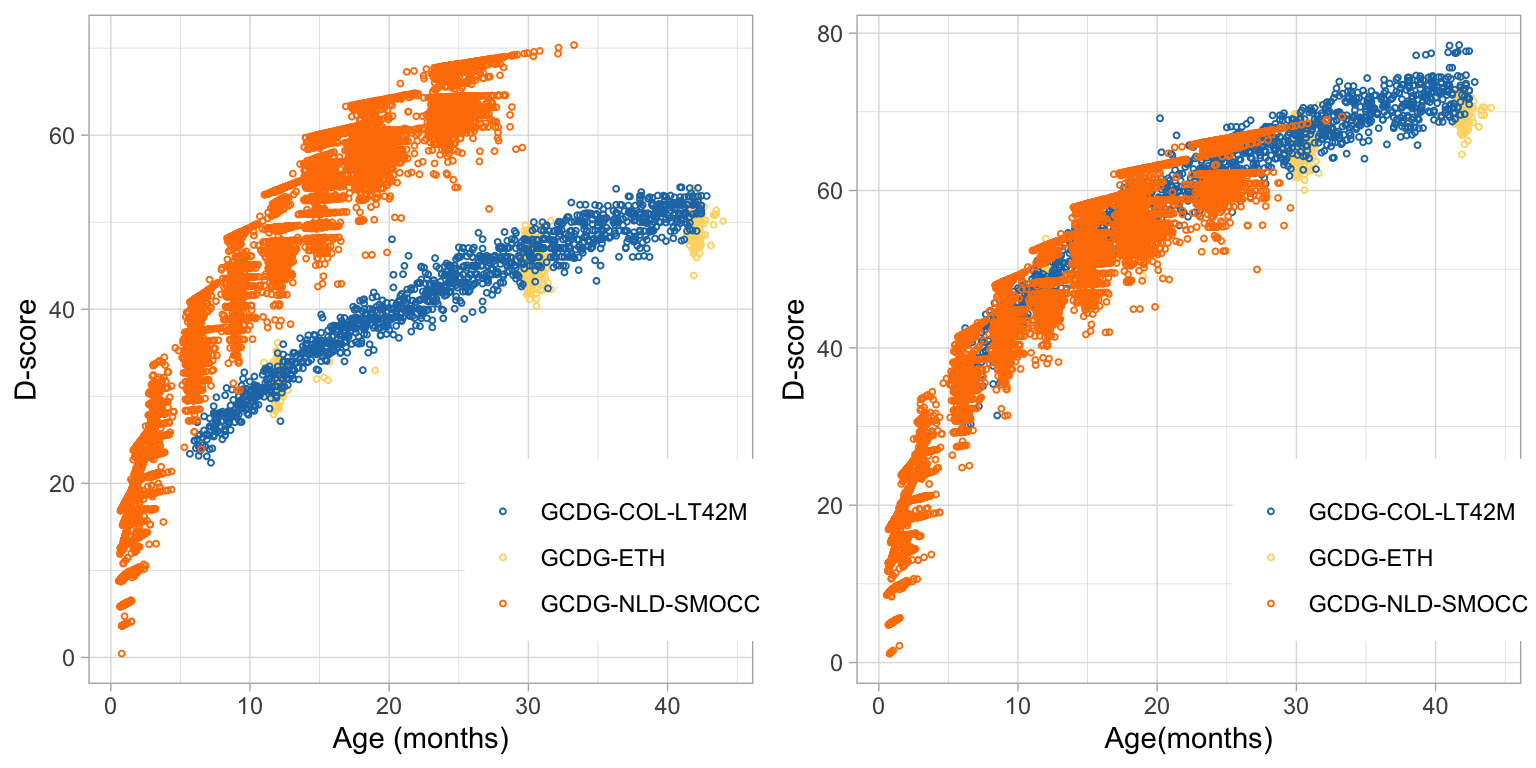
\includegraphics[width=1\linewidth]{dbook2_files/figure-latex/commonscale-1} 

}

\caption{Example of three cohorts with and without equate group linking.}\label{fig:commonscale}
\end{figure}



Figure \ref{fig:commonscale} displays the D-score estimates by age in three cohorts from the GCDG study: Netherlands 1 (GCDG-NLS-SMOCC), Ethiopia (GCDG-ETH) and Colombia 2 (GCDG-COL-LT42M) for two different analyses. As described in section \ref{sec:cohorts}, the Netherlands 1 study administered the \texttt{ddi}; Ethiopia measured children by the \texttt{by3}; and Colombia collected data on \texttt{by3}, \texttt{den}, \texttt{aqi} and \texttt{bdi}. Accordingly, there is an overlap in items between Ethiopia and Colombia via the \texttt{by3}, but the Netherlands 1 cohort is not linked.

We created the plot on the left-handed side without active equate groups. The large overlap between Ethiopian and Columbian children occurs because the scales for these studies are linked naturally via shared items from \texttt{by3}. Since the \texttt{ddi} instrument is not connected, the Dutch cohort follows a different track. While we can compare D-scores between Ethiopia and Colombia, it is nonsensical to compare Dutch to either Ethiopia or Colombia. The right-handed side plot is based on an analysis that used active equate groups to link the cohorts. Since the analysis connected the scales for all three cohorts, we can now compare D-scores obtained between all three cohorts.

This example demonstrates that active equate groups form the key for converting ability estimates for children from different cohorts using different instruments onto the same scale.

\hypertarget{sec:equatefit}{%
\section{Quantifying equate fit}\label{sec:equatefit}}

It is essential to activate only those equate groups for which the assumption of equivalent measurement holds. We have already seen the \emph{item fit} and \emph{person fit} diagnostics of the Rasch model. This section describes a similar measure for the quality of an active equate group.

\hypertarget{equate-fit}{%
\subsection{Equate fit}\label{equate-fit}}

\href{https://d-score.org/dbook1/ch-evaluation.html}{Chapter 6 of booklet I} defines the observed response of person \(n\) on item \(i\) as \(x_{ni}\). The accompanying standardized residual \(z_{ni}\) is the difference between \(x_{ni}\) and the expected response \(P_{ni}\), divided by the expected binomial standard deviation,

\[z_{ni} = \frac{x_{ni}-P_{ni}}{\sqrt{W_{ni}}},\]

with variances \(W_{ni} = P_{ni}(1-P_{ni})\).

\emph{Equate infit} is an extension of item infit that takes an aggregate over all items \(i\) in active equate group \(g\), i.e.,

\[\mathrm{Equate\ infit} = \frac{\sum_{i\in g}\sum_{n}^N (x_{ni}-P_{ni})^2}{\sum_{i\in g}\sum_n^N W_{ni}}.\]

Likewise, we calculate \emph{Equate outfit} of group \(g\) as

\[\mathrm{Equate\ outfit} = \frac{\sum_{i\in g}\sum_{n}^{N_i} z_{ni}^2}{\sum_{i\in g} N_i},\]

where \(N_i\) is the total number of responses observed on item \(i\). The interpretation of these diagnostics is the same as for item infit and item outfit.

Note that these definitions implicitly assume that the expected response \(P_{ni}\) is calculated under a model in which all items in equate group \(g\) have the same difficulty. This is not true for passive equate groups. Of course, no one can stop us from calculating the above equate fit statistics for passive groups, but such estimates would ignore the between-item variation in difficulties, and hence gives a too optimistic estimate of quality. The bottom line is: \emph{The interpretation of the equate fit statistics should be restricted to active equate groups only}.

\hypertarget{examples-of-well-fitting-equate-groups}{%
\subsection{Examples of well fitting equate groups}\label{examples-of-well-fitting-equate-groups}}

The evaluation of \emph{equate fit} involves comparing the observed probabilities of endorsing the items in the equate group to the estimated probability of endorsing the items in the equate group. For an equate group there is an empirical curve for each item in the equate group and one shared estimated curve. The empirical curves should all be close together, and close to the estimated curve for a good equate fit.

\begin{figure}

{\centering 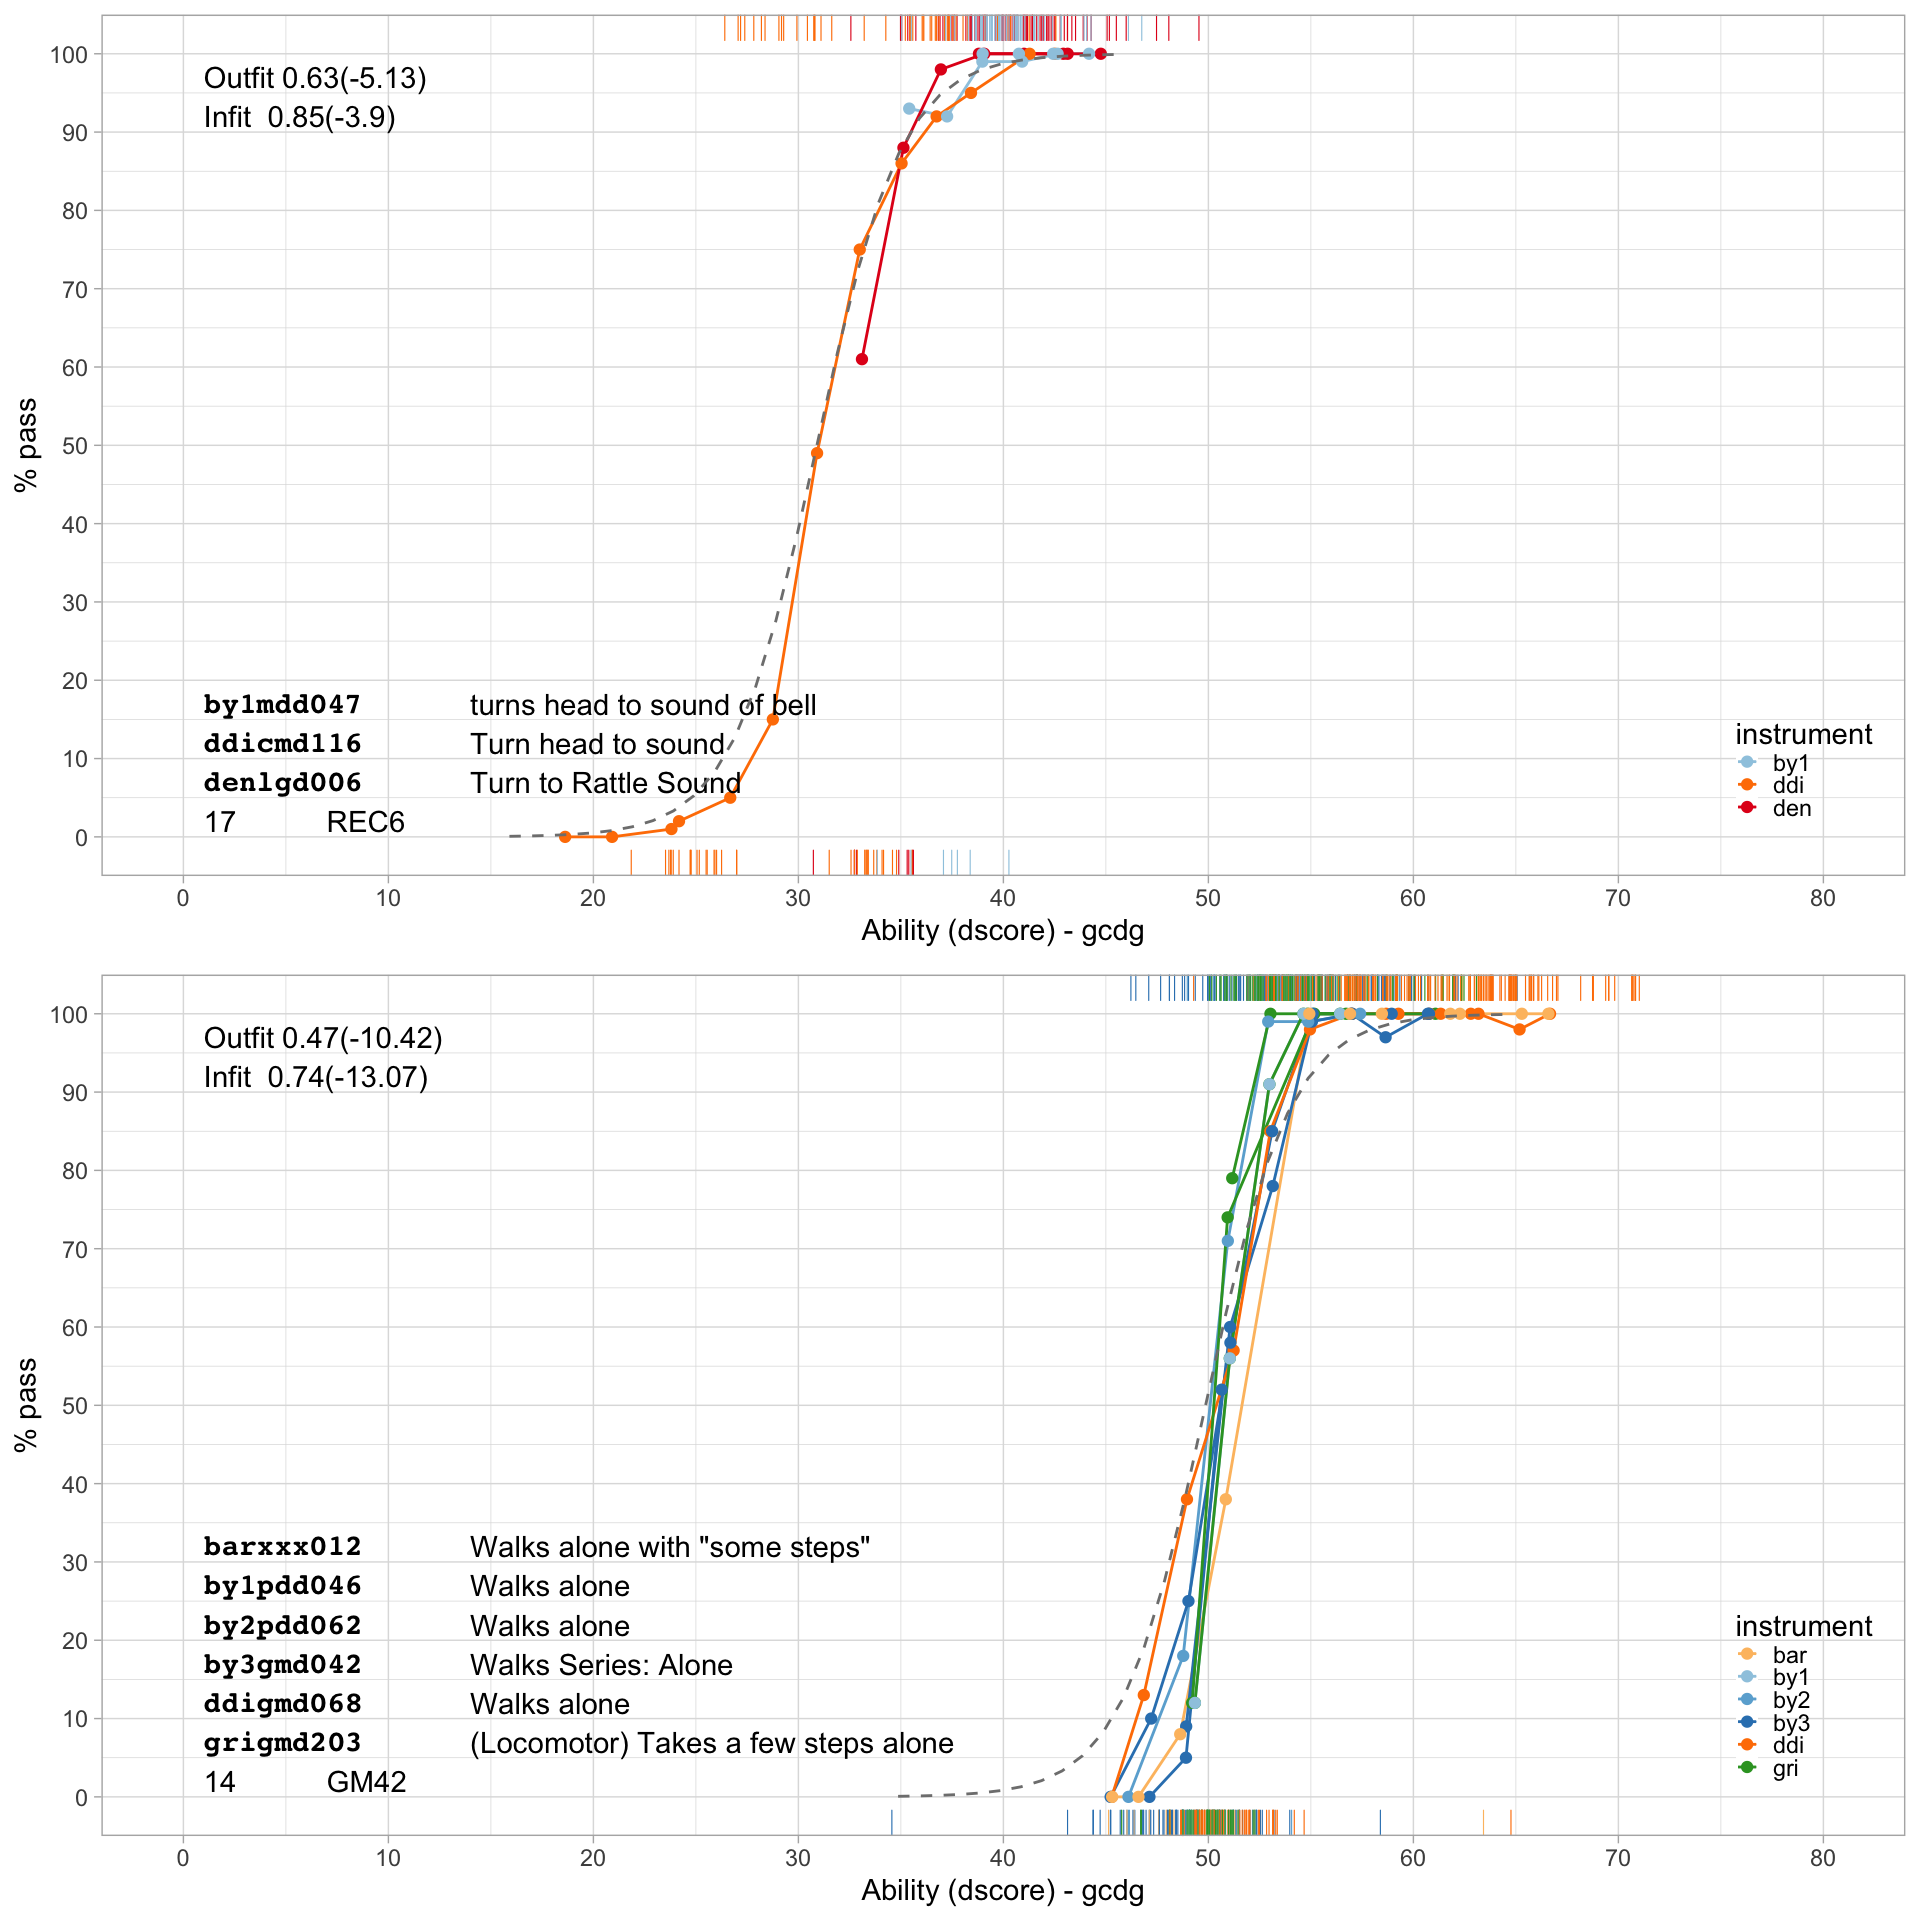
\includegraphics[width=1\linewidth]{dbook2_files/figure-latex/ploteqfit-1} 

}

\caption{Two equate groups that present a good equate fit.}\label{fig:ploteqfit}
\end{figure}



Figure \ref{fig:ploteqfit} shows a diagnostic plot for equate groups \texttt{REC6} (Turns head to sound of bell) and \texttt{GM42} (Walks alone). The items within \texttt{REC6} have slightly different formats in the Bayley I (\texttt{by1}), Dutch Development Instrument (\texttt{ddi}), and the Denver (\texttt{den}). The empirical curves in the upper figure show good overlap, but note that hardly any negative responses were recorded for four of the five studies, so the shared estimate depends primarily on the Dutch sample. Items from equate group \texttt{GM42} appear in six instruments: \texttt{bar}, \texttt{by1}, \texttt{by2}, \texttt{by3}, \texttt{ddi}, and \texttt{gri}. Also, here the empirical data are close together, and even a little steeper than the fitted dashed line, which indicates a good equate fit. The infit and outfit indices, shown in the upper left corners, confirm the good fit (fit \textless{} 1).

\hypertarget{examples-of-equate-groups-with-poor-equate-fit}{%
\subsection{Examples of equate groups with poor equate fit}\label{examples-of-equate-groups-with-poor-equate-fit}}

Poor fitting equate groups are best treated as passive equate groups, so that items in those groups are not restricted to the same difficulty. Empirical item curves with different locations and slopes indicate a poor fit. Additionally, the equate fit indices will indicate a poor fit (fit \textgreater{} 1).

\begin{figure}

{\centering 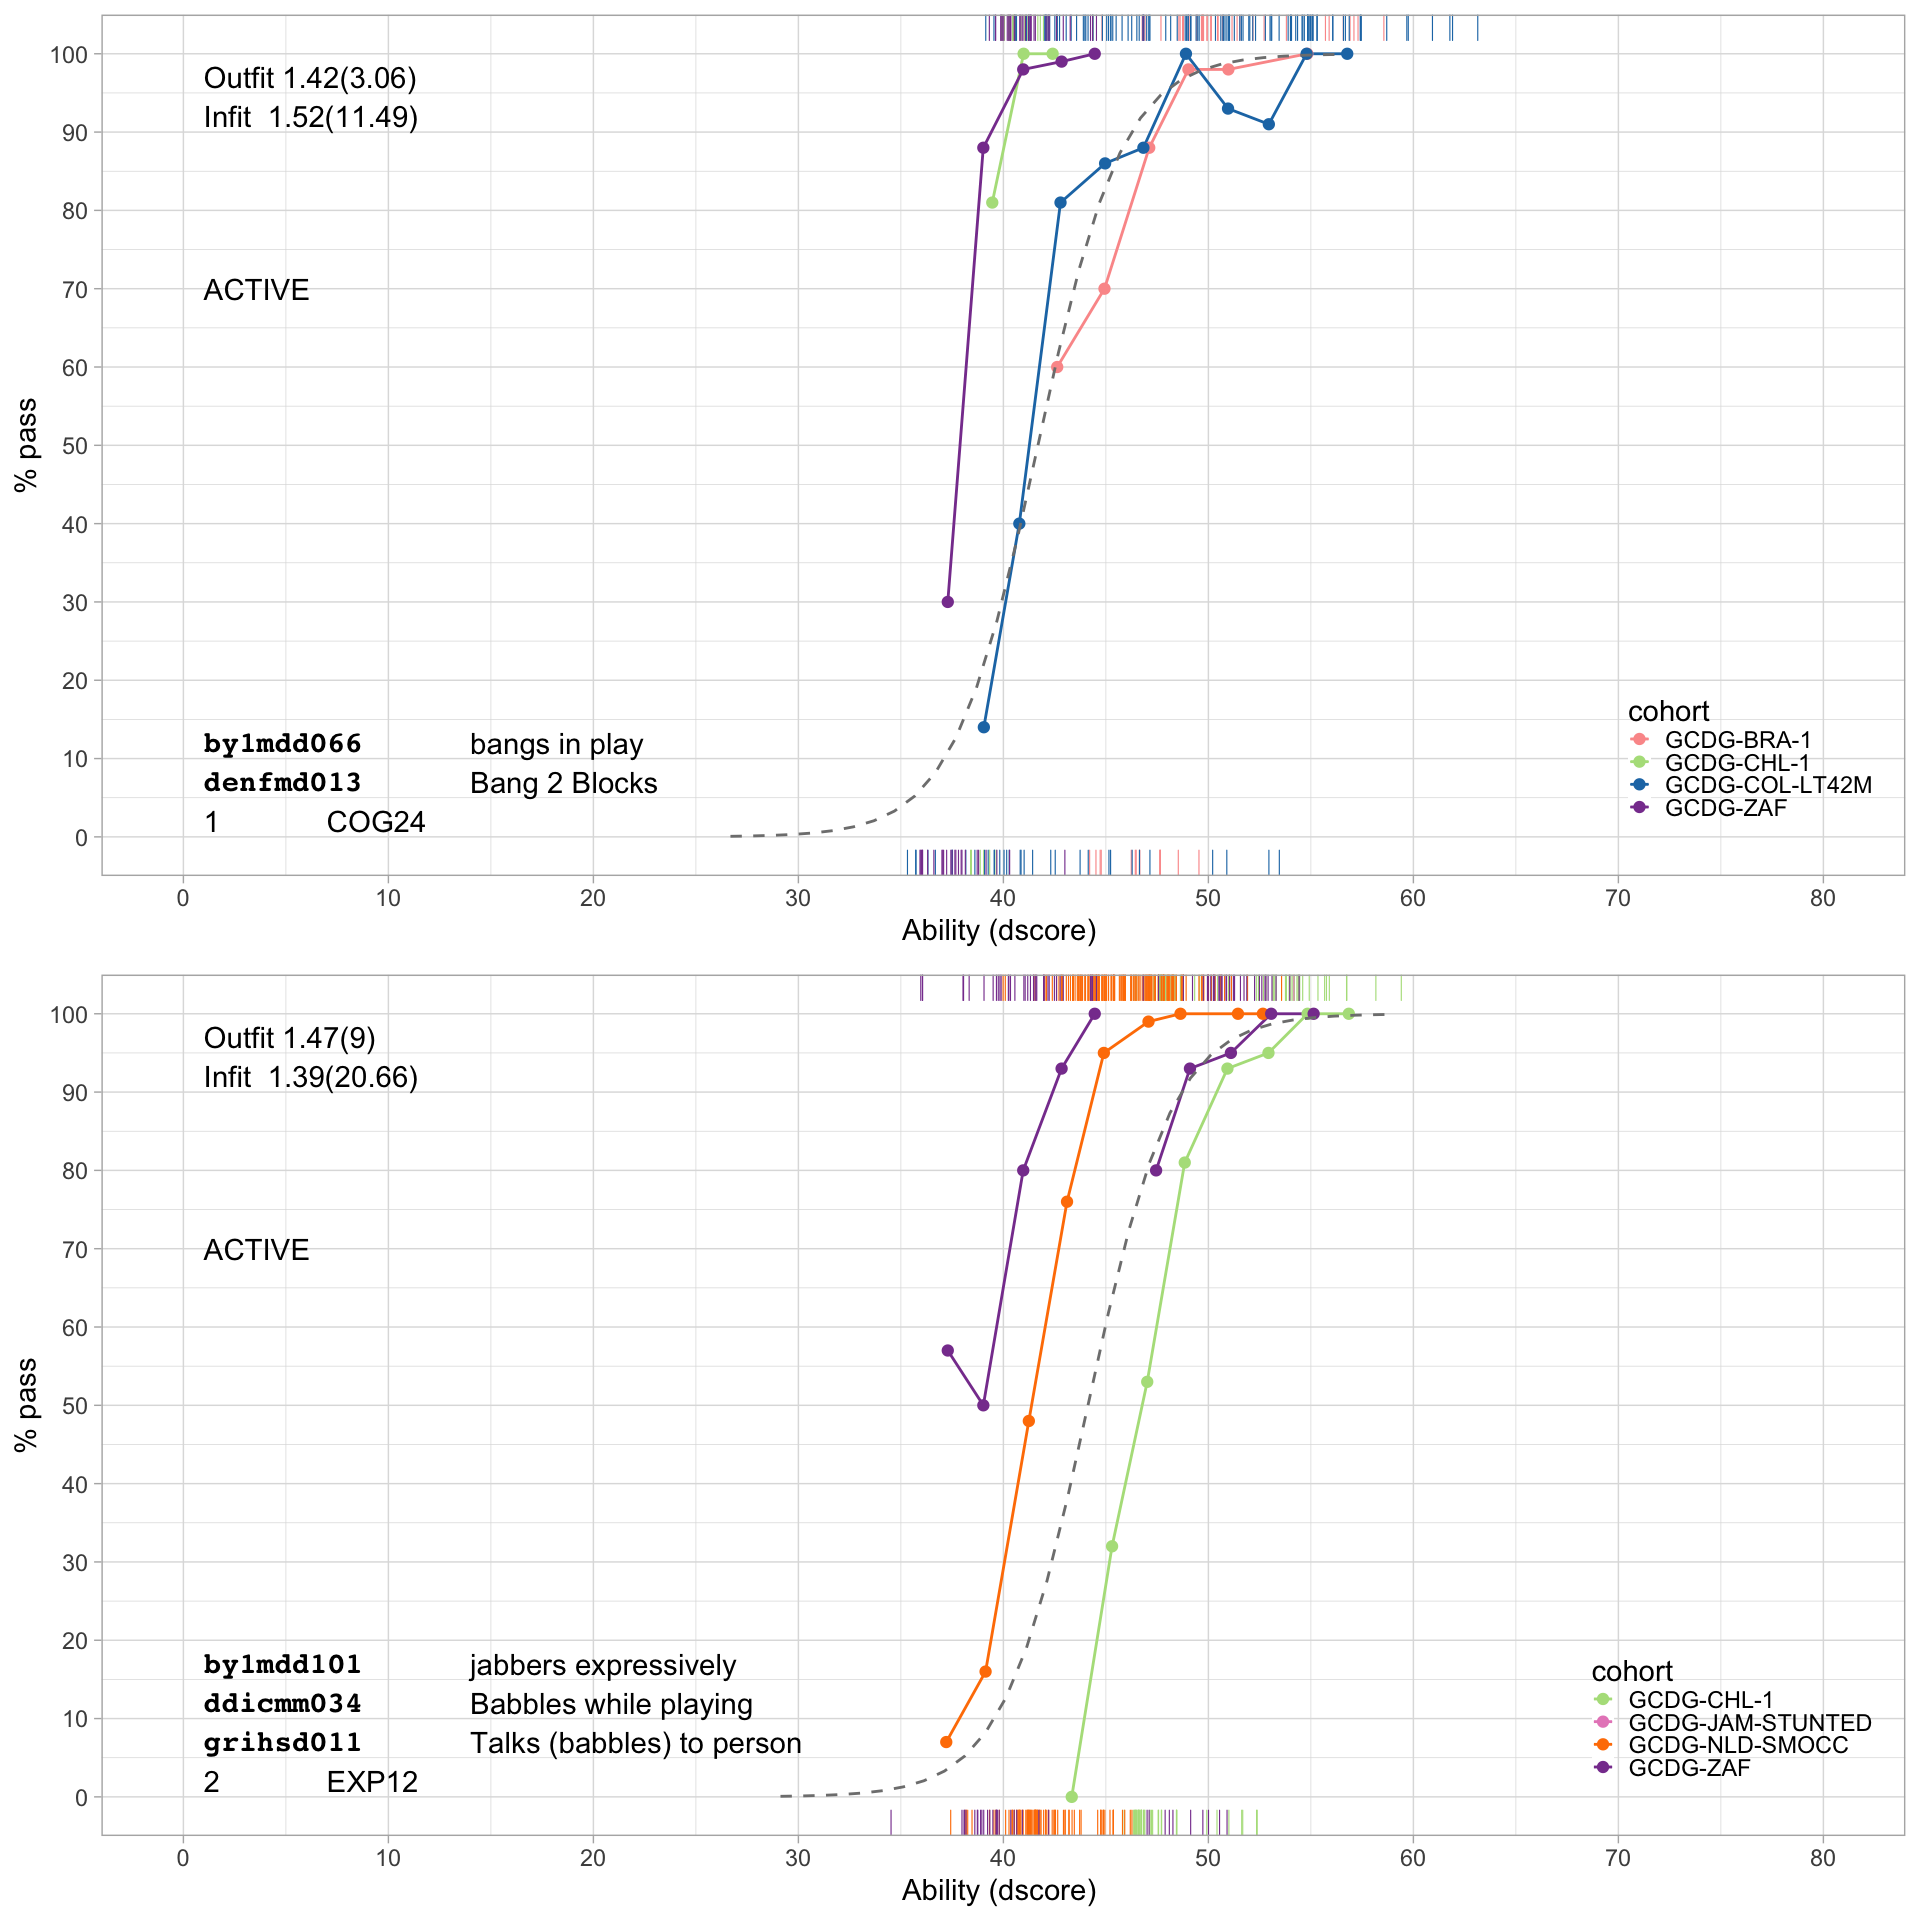
\includegraphics[width=1\linewidth]{dbook2_files/figure-latex/ploteqpoor-1} 

}

\caption{Two equate groups that present a poor equate fit.}\label{fig:ploteqpoor}
\end{figure}



Figure \ref{fig:ploteqpoor} shows examples for groups \texttt{COG24} (Bangs in play / Bangs 2 blocks) and \texttt{EXP12} (Babbles). In both cases there is substantial variation in location between the empirical curves. For \texttt{COG24} we find that the fitted curve is closer to the \texttt{den} item, which suggests that the equate difficulty is mostly based on the \texttt{den} item. Items from equate group \texttt{EXP12} have a different format in instruments \texttt{by1}, \texttt{ddi}, and \texttt{gri}. The empirical curves, with different colours for each instrument, are not close to each other, nor close to the fitted curve. Note that all infit and outfit statistics are fairly high, indicating poor fit. Both equates are candidates for deactivation in a next modelling step.

\hypertarget{sec:equatedif}{%
\section{Differential item functioning}\label{sec:equatedif}}

Items within an active equate group should work in the same way across the different cohorts, i.e., they have no differential item functioning (DIF). The assumption of no DIF is critical for active equate groups. If violated, restricting the difficulty parameters as equal across cohorts may introduce unwanted bias in comparisons between cohorts. This section illustrates the role of DIF in equate groups.

\hypertarget{good-equate-groups-without-dif}{%
\subsection{Good equate groups without DIF}\label{good-equate-groups-without-dif}}

\href{https://d-score.org/dbook1/sec-dif.html}{Booklet I} discusses the role of DIF in the evaluation of the fit of items to the Rasch model. This section illustrates similar issues in the context of equate groups.

\begin{figure}

{\centering 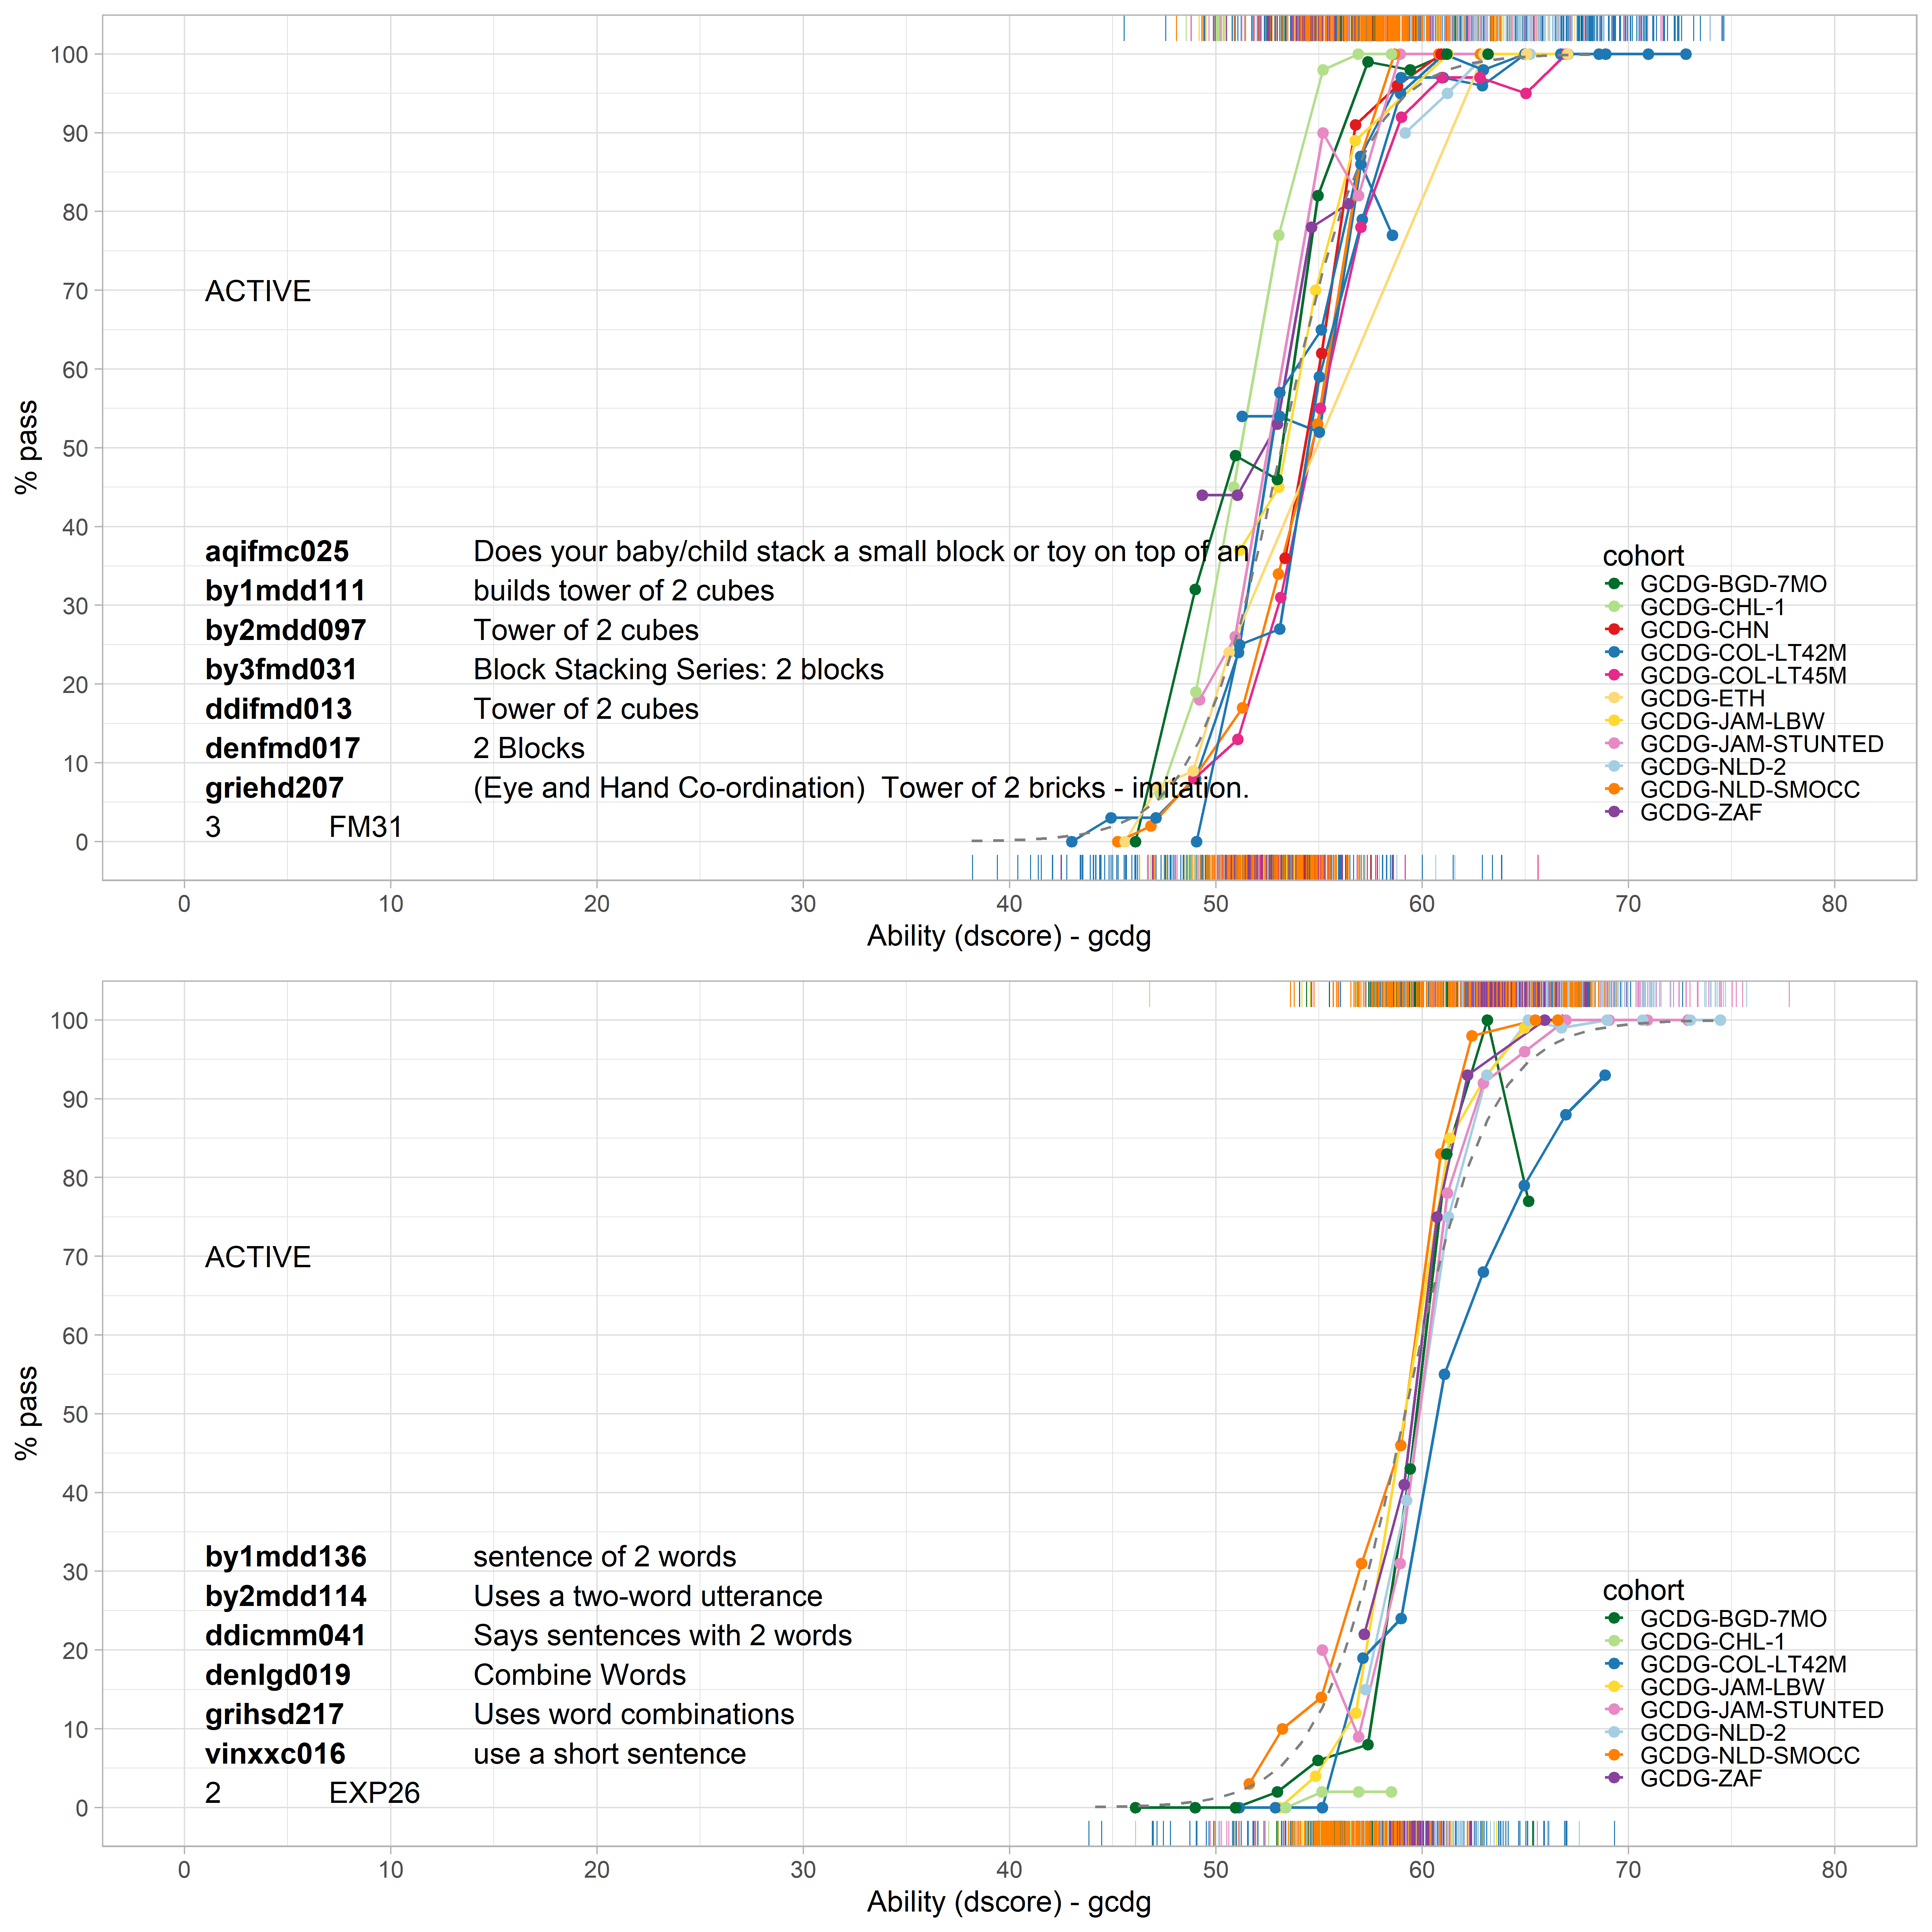
\includegraphics[width=1\linewidth]{dbook2_files/figure-latex/plotnoeqdif-1} 

}

\caption{Two equate groups that present no differential item functioning between cohorts.}\label{fig:plotnoeqdif}
\end{figure}



Figure \ref{fig:plotnoeqdif} shows the empirical curves of two equate groups, \texttt{FM31} (two cubes) and \texttt{EXP26} (two-word sentence). All curves are close to each other, so there is no differential item functioning here.

\hypertarget{poor-equate-groups-with-dif-for-study}{%
\subsection{Poor equate groups with DIF for study}\label{poor-equate-groups-with-dif-for-study}}

\begin{figure}

{\centering 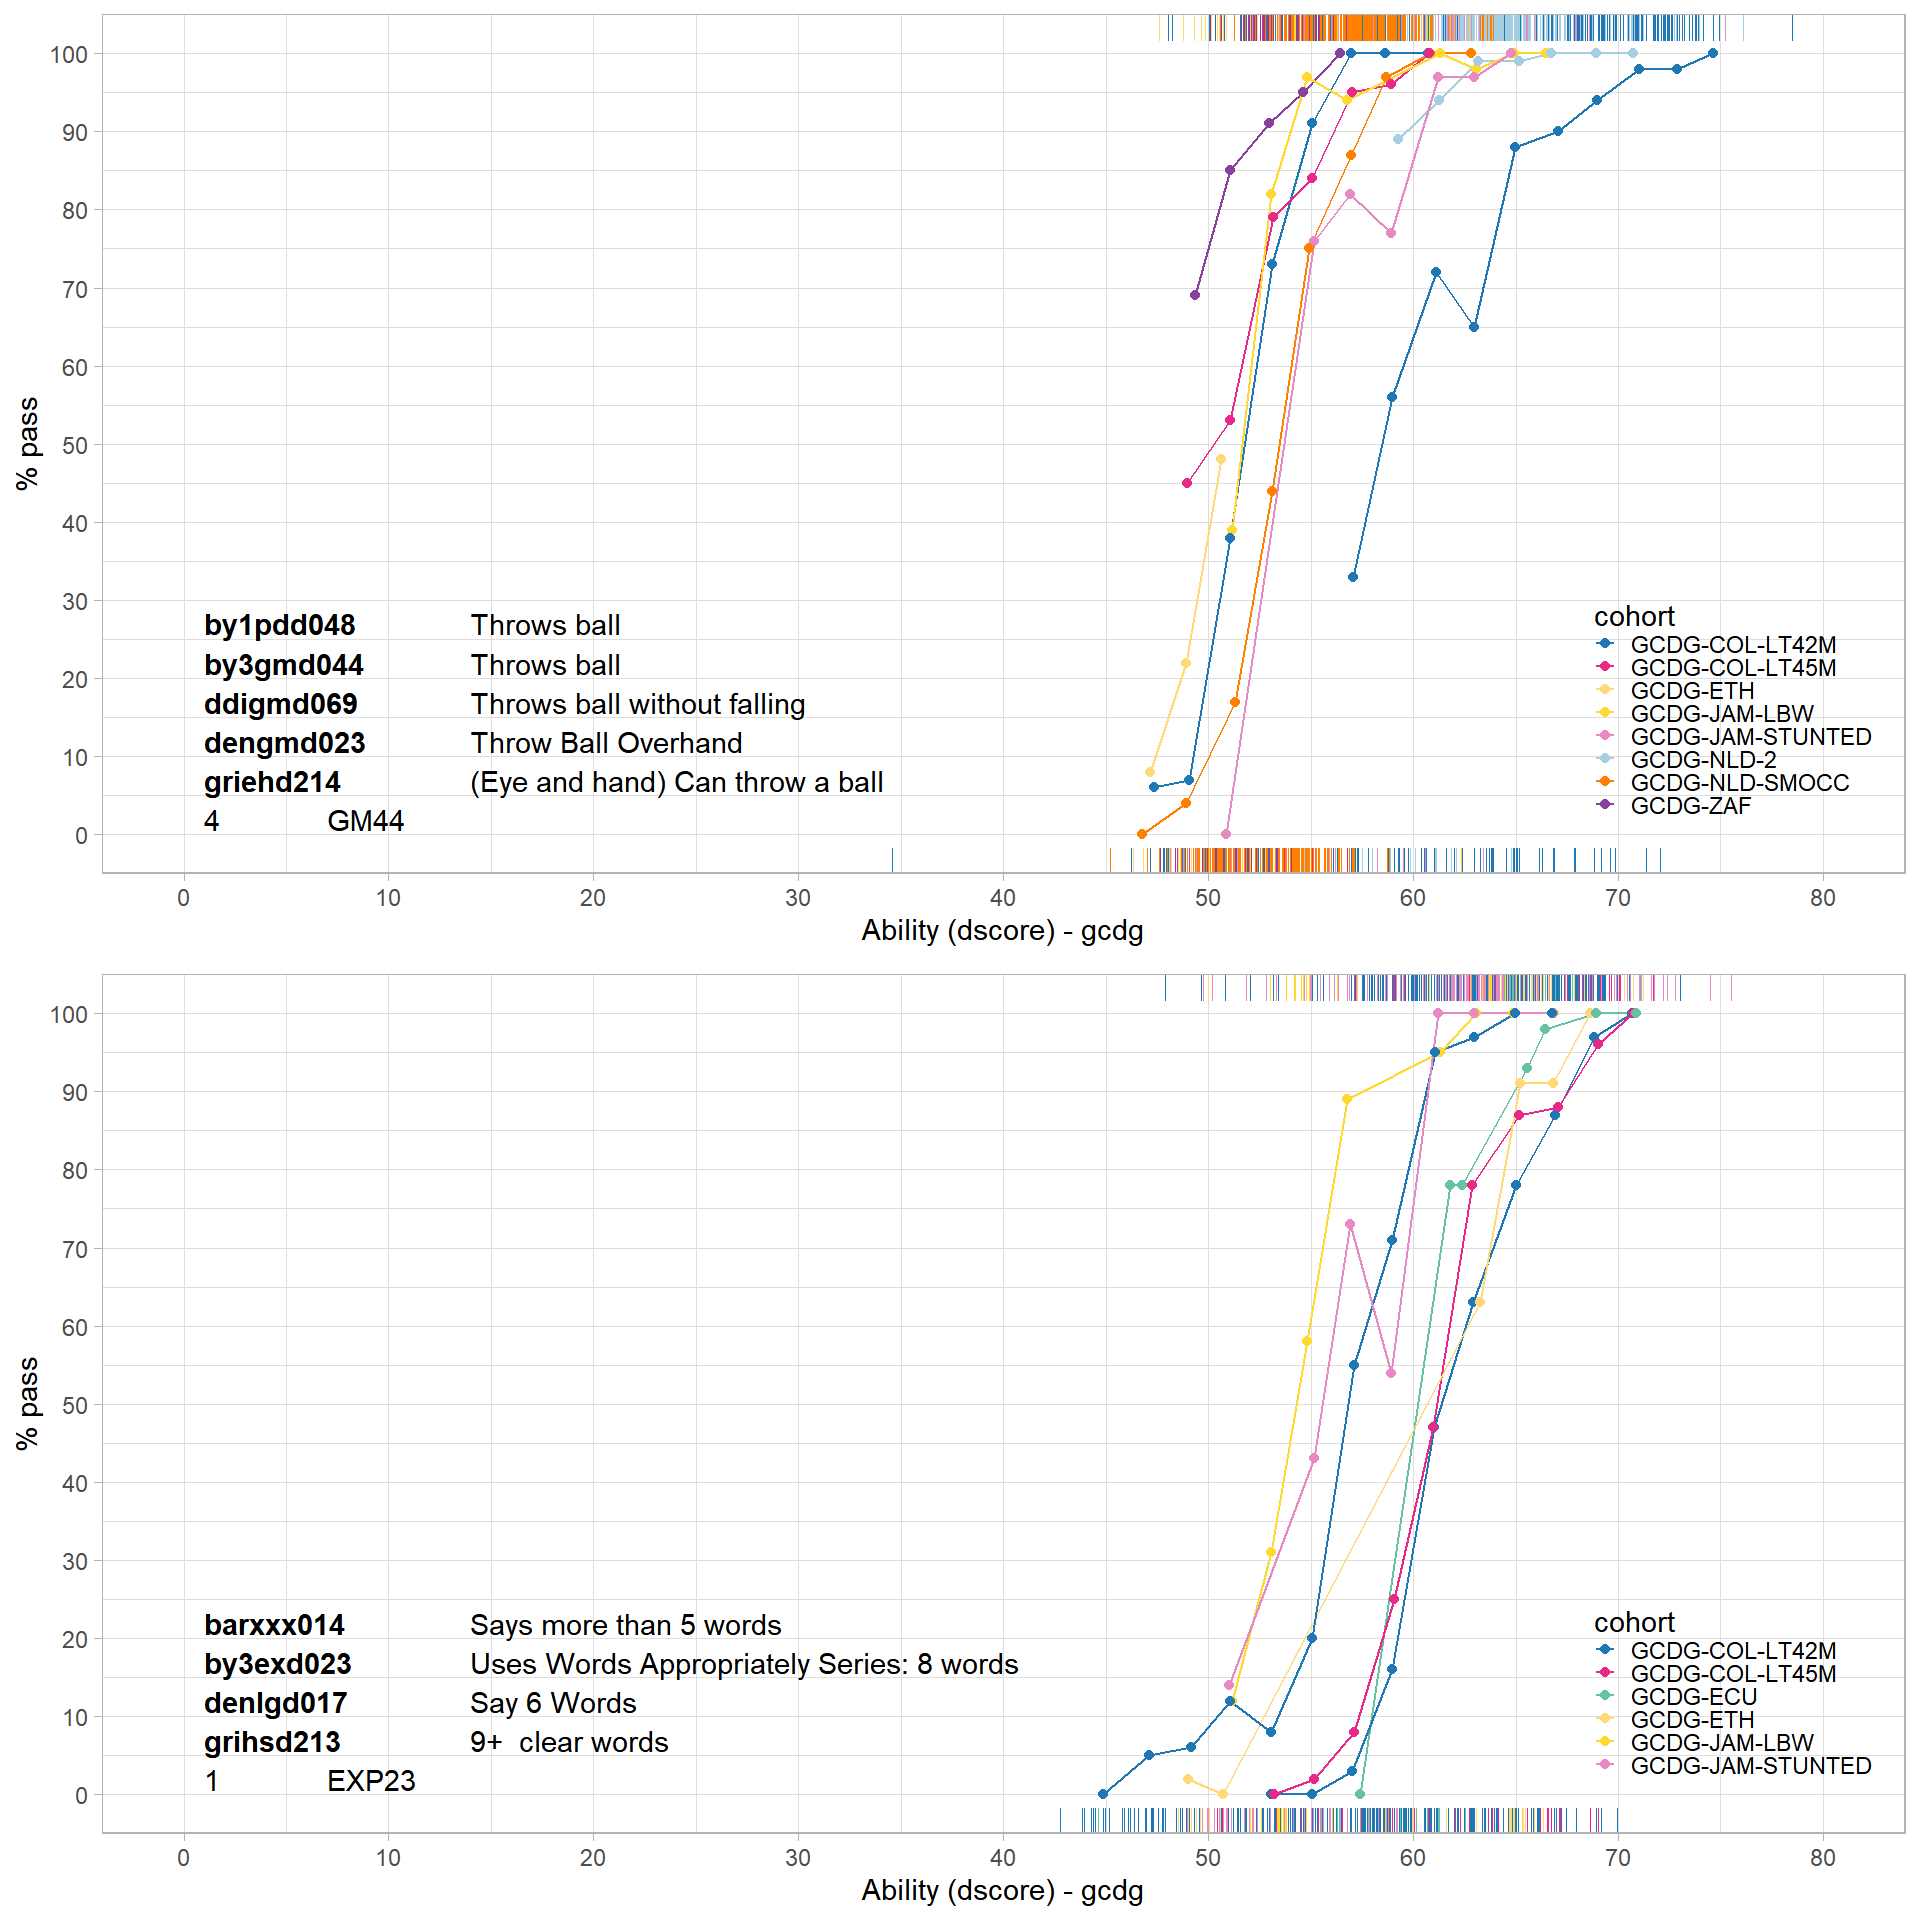
\includegraphics[width=1\linewidth]{dbook2_files/figure-latex/ploteqdif-1} 

}

\caption{Two equate groups that present differential item functioning between cohorts.}\label{fig:ploteqdif}
\end{figure}



Figure \ref{fig:ploteqdif} plots the empirical curves for equate groups \texttt{GM44} (throws ball) and \texttt{EXP23} (5 or more words). The substantial variation between these curves is a sign of differential item functioning. For example, \emph{Throws ball} is easier for children in the South-Africa cohort (purple curve; GCDG-ZAF) and more difficult for children in Colombia (blue curve; GCDG-COL-LT42M). In other words, the probability of passing the item given the D-score (i.e.~item difficulty) differs between the cohorts. Likewise, there is differential item functioning for \emph{Says more than 5 words}. This milestone is easier for children in Jamaica (yellow and pink curves; GCDG-JAM-LBW and GCDG-JAM-STUNTED) than for children from Ecuador (green; GCDG-ECU).

\hypertarget{ch:modellingequates}{%
\chapter{Modelling equates}\label{ch:modellingequates}}

\begin{quote}
Author: Stef van Buuren, Iris Eekhout
\end{quote}

This chapter deals with the nitty-gritty of the modelling strategy used for the GCDG data introduced in chapter \ref{ch:data}. This chapter

\begin{itemize}
\tightlist
\item
  provides a high-level description of the GCDG data (\ref{sec:gcdgdata})
\item
  discusses various modelling strategies (\ref{sec:modellingstrategies})
\item
  shows the impact of equate groups on the model in extreme cases (\ref{sec:impactequate})
\item
  demonstrates visualisation of age profiles to select promising equate groups (\ref{sec:ageprofiles})
\item
  introduces a helpful visualisation of the quality of the equate group (\ref{sec:equatequality})
\item
  highlights infit and outfit for removing misfitting milestones (\ref{sec:milestoneselection})
\item
  discusses instrument fit and equate group editing (\ref{sec:othermodelling})
\item
  introduces a grading system for equate groups (\ref{sec:iteminformation})
\item
  provides pointers to the final model (\ref{sec:finalmodel})
\end{itemize}

\hypertarget{sec:gcdgdata}{%
\section{GCDG data: design and description}\label{sec:gcdgdata}}

\hypertarget{data-combination}{%
\subsection{Data combination}\label{data-combination}}

Section \ref{sec:gcdgoverview} provides an overview of the data collected by Global Child Development Group. The group collected item level measurements obtained on 12 instruments for measuring child development across 16 cohorts.

We coded every item as 0 (FAIL), 1 (PASS) or missing. For some instrument we did some additional recoding to restrict to these two response categories. The Battelle Developmental Inventory scores items as 0 (FAIL), 1, or 2, depending on the level of skill demonstrated or time taken to complete the task. We joined categories 1 and 2 for these items. The ASQ items were originally scored as 0 (not yet), 5 (sometimes) and 10 (succeeds). We recoded both 5 and 10 to 1.

We concatenated the datasets from the GCDG cohorts cohort. The resulting data matrix has 71403 rows (child-visit combinations) and 1572 columns (items) collected from 36345 unique children. We removed 233 items that had fewer than 10 observations in a category. The remaining 1339 items were candidates for analysis. The total number of observed scores was equal to about 2.8 million pass/fail responses. While this is a large number of measurements, about 97 percent of the entries in the matrix are missing.

\hypertarget{equate-group-formation}{%
\subsection{Equate group formation}\label{equate-group-formation}}

A group of 13 subject-matter experts from the Global Child Development Group cross-walked the available instruments for similar milestones. This group

\begin{itemize}
\tightlist
\item
  developed an item coding schema;
\item
  matched similarly appearing items stemming from different instruments;
\item
  formed an opinion about the quality of each match;
\item
  noted peculiarities of the matches;
\item
  reported the results as a series of detailed Excel spreadsheets.
\end{itemize}

\begin{figure}

{\centering 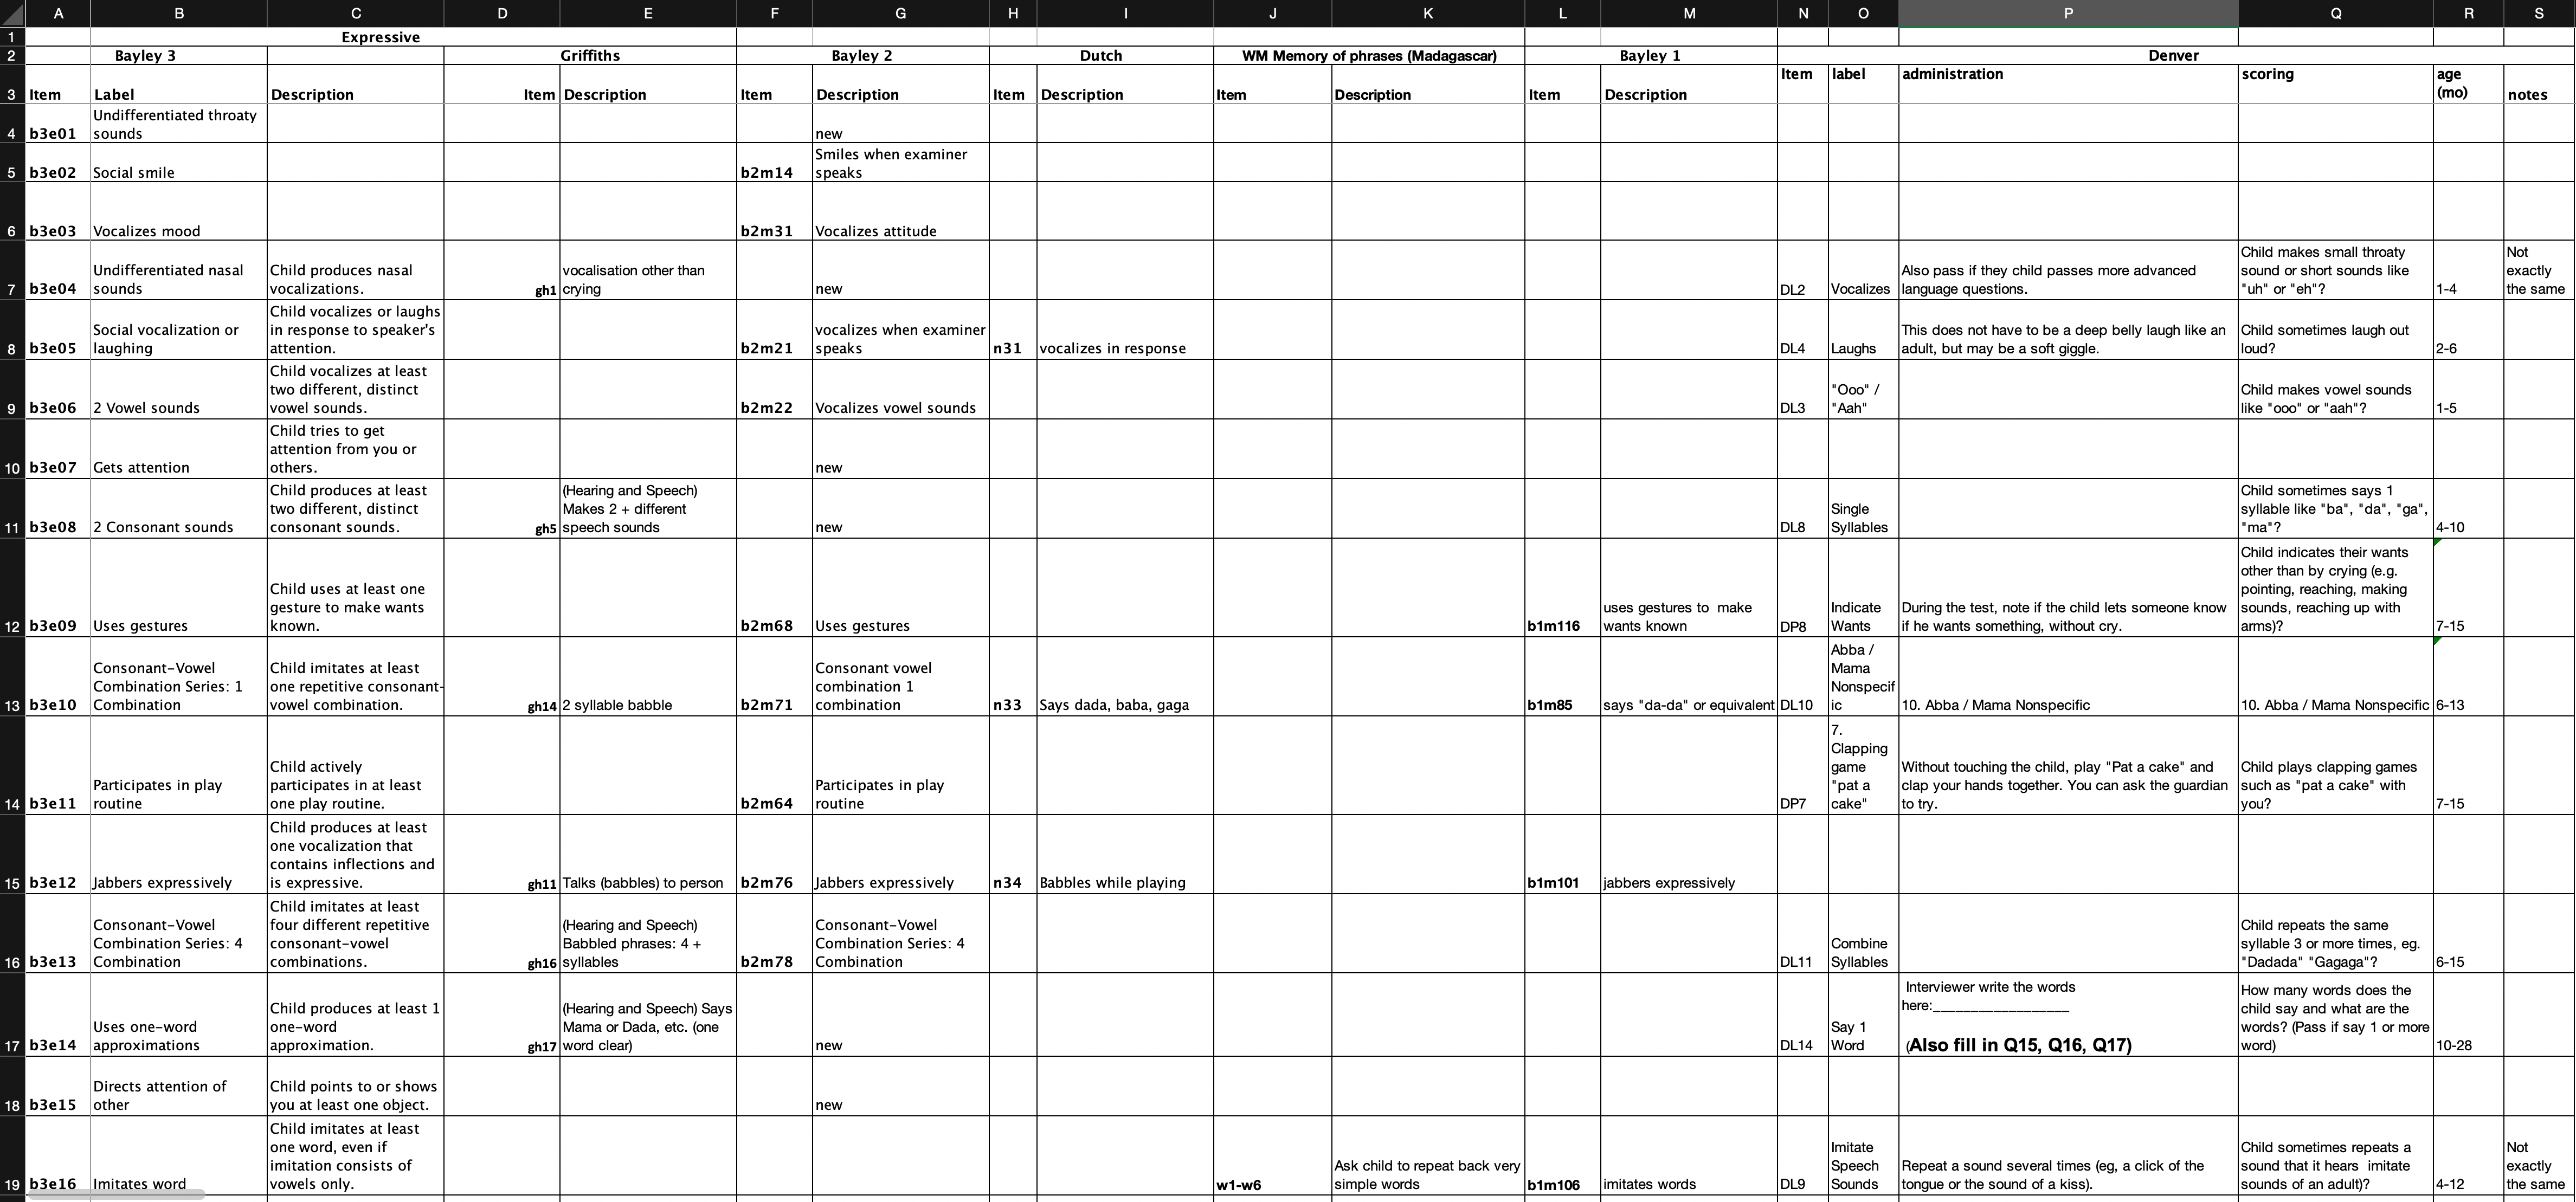
\includegraphics[width=1\linewidth]{fig/equate_excel} 

}

\caption{A snapshot of information generated by subject-matter experts.}\label{fig:equatesheetpic}
\end{figure}



The group evaluated around 1500 milestones. After several days, this highly-skilled, intensive labour resulted in a series of spreadsheets. Figure \ref{fig:equatesheetpic} shows an example. These sheets formed the basis of an initial list of 184 equate groups, each consisting of at least two items.

\hypertarget{sec:modellingstrategies}{%
\section{Modelling strategies}\label{sec:modellingstrategies}}

The analytic challenge is twofold:

\begin{itemize}
\tightlist
\item
  to find a subset of items that form a scale;
\item
  to find a subset of equate groups with items similar enough to bridge instruments.
\end{itemize}

Note that both subsets are related, i.e., changing one affects the other. Thus, we cannot first identify items and then equate groups, or first identify equate groups followed by the items. Rather we need to find the two subsets in an iterative fashion, primarily by hand. This chapter describes some of the modelling issues the analyst needs to confront.

In general, we look for a final model that

\begin{itemize}
\tightlist
\item
  preserves the items that best fit the Rasch model;
\item
  uses active equate groups with items that behave the same across many cohorts and instruments;
\item
  displays reasonable age-conditional distributions of the D-scores;
\item
  has difficulty estimates that are similar to previous estimates.
\end{itemize}

The modelling strategy is a delicate balancing act to achieve all of the above objectives. Particular actions that we could take to improve a given model are:

\begin{itemize}
\tightlist
\item
  remove bad items;
\item
  inactivate bad equate groups;
\item
  break up bad equate groups;
\item
  move items from one equate group to another;
\item
  create new equate groups;
\item
  remove entire instruments;
\item
  remove persons;
\item
  remove studies.
\end{itemize}

In order to steer our actions, we look at the following diagnostics (in order of importance):

\begin{itemize}
\tightlist
\item
  quality of equate groups (both visually and through infit);
\item
  plausibility of the distribution of the D-score by age per study;
\item
  correspondence of difficulty estimates from published (single study) Dutch data and the new model;
\item
  infit of the items remaining in the model.
\end{itemize}

Various routes are possible and may result in different final models. The strategy adopted here is to thicken active equate groups by covering as many studies as possible, in the hope of minimizing the number of active equates needed.

\hypertarget{sec:impactequate}{%
\section{Impact of number of active equate groups}\label{sec:impactequate}}

\begin{figure}

{\centering 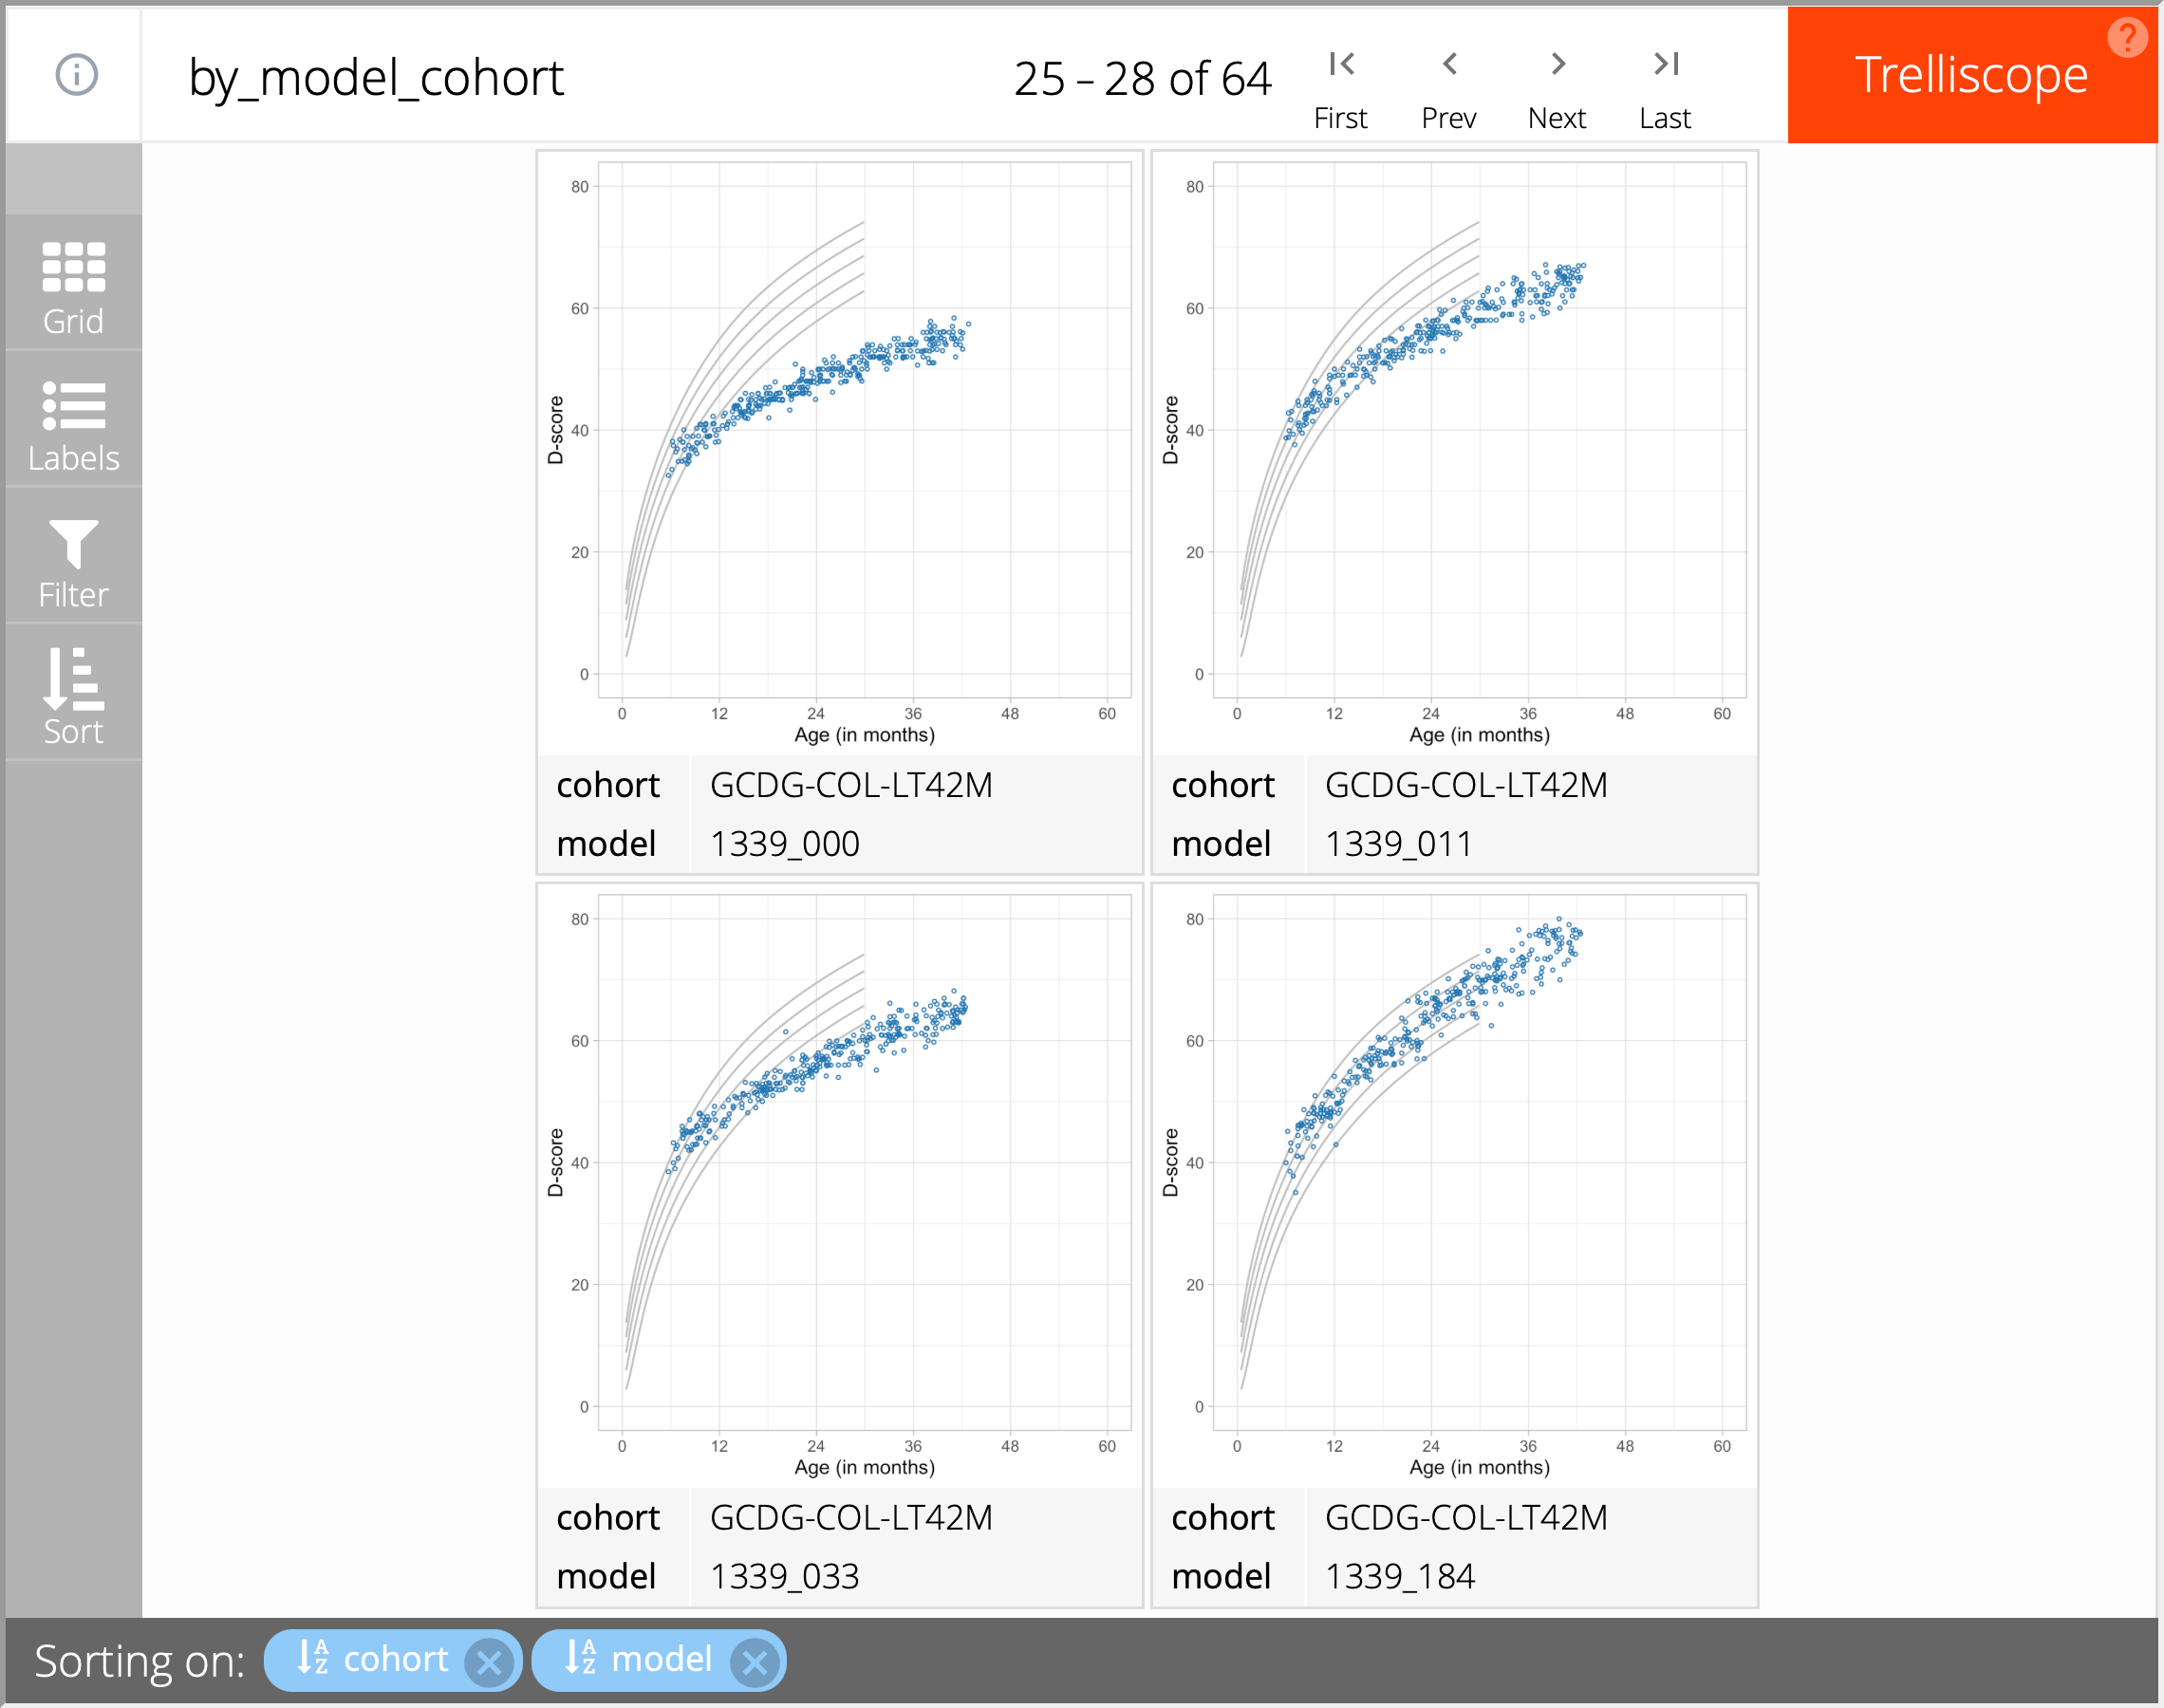
\includegraphics[width=1\linewidth]{fig/fig_5.2} 

}

\caption{\href{https://d-score.org/dbook-apps/models1339/\#display=by_model_cohort\&nrow=2\&ncol=2\&arr=row\&pg=7\&labels=cohort,model\&sort=cohort;asc,model;asc\&filter=\&sidebar=\&fv=}{D-score by age of four models with all 1339 items using 0, 11, 33 and 184 active equate groups. The number of equate groups has a substantial effect on the D-score distribution. Use the arrows to see other cohorts} (\url{https://d-score.org/dbook-apps/models1339/}).}\label{fig:model1339}
\end{figure}



Figure \ref{fig:model1339} is a display of the D-score by age for all 16 cohorts under four models. As a rough reference to compare, the grey curves in the back represent the Dutch model as calculated from the \href{https://d-score.org/dbook1/sec-smoccstudy.html}{SMOCC study}. In order to speed up the calculations, the figure shows a random subsample of 25\% of all points. Manipulate the plot controls to switch cohorts.

All models contain 1339 items, but differ in the number of active equate groups. The most salient features per model are:

\begin{itemize}
\tightlist
\item
  \texttt{1339\_0}: No equate groups, so different instruments in different cohorts are fitted independently;
\item
  \texttt{1339\_11}: Connects all cohorts through one or more equated items using 11 equate groups in total;
\item
  \texttt{1339\_33}: There are 33 equate groups that bridge cohort and instruments;
\item
  \texttt{1339\_184}: Maximally connects instruments and cohort by all equate groups.
\end{itemize}

Comparison of the D-score distribution by age across these models yields various insights:

\begin{itemize}
\item
  The location of cohorts on the vertical scale depends on the number of active equate groups. For example, for Madagascar (MDG) the points are located around 52 when no equate groups are activated, whereas if all are activated it is about 68.
\item
  The age trend depends on the number of active equate groups. For example, for Colombia (COL) or Ethiopia (ETH), the model without equate groups has a shallow age trend, whereas it is steep for the \texttt{1339\_184} model.
\item
  The vertical spread depends on the number of equate groups. For example, the spread in the Chile-2 (CHL-2) cohort substantially increases with the number of active equates.
\item
  Model \texttt{1339\_0} for the Dutch NLD-SMOCC cohort is equivalent to the model fitted to the \href{https://d-score.org/dbook1/sec-smoccstudy.html}{SMOCC study} alone. Introducing equate groups compresses the range of scores, especially at the higher end.
\end{itemize}

We have now seen that the number of active equate groups has a large effect on the model. The next sections look into the equate groups in more detail.

\hypertarget{sec:ageprofiles}{%
\section{Age profiles of similar milestones}\label{sec:ageprofiles}}

\begin{figure}

{\centering 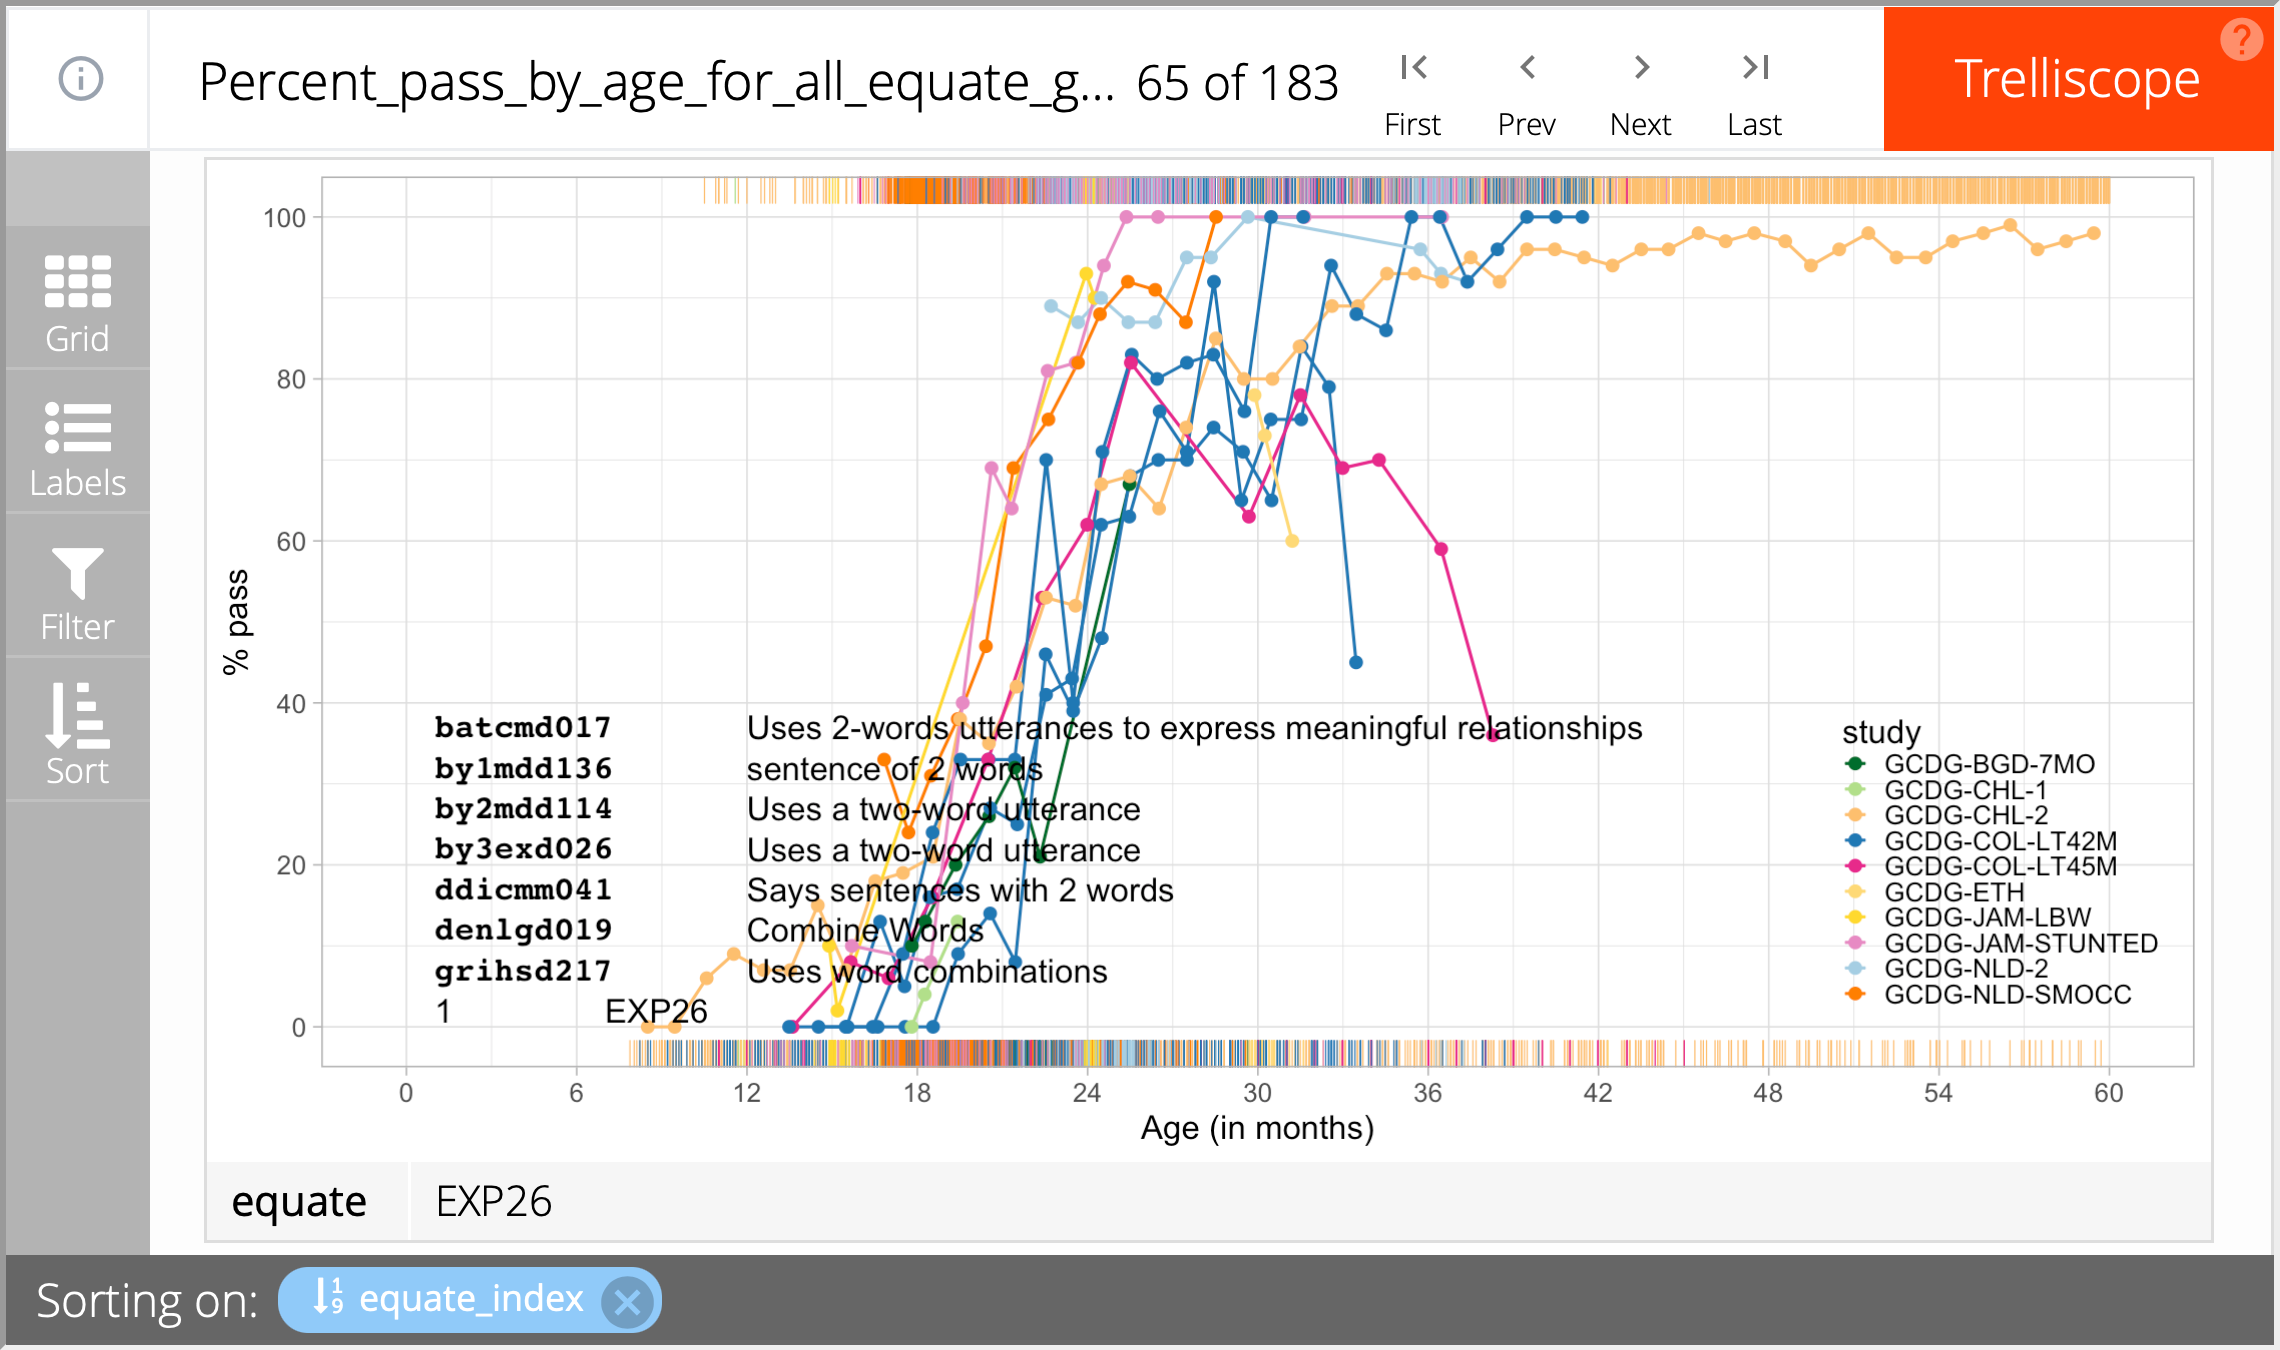
\includegraphics[width=1\linewidth]{fig/fig_5.3} 

}

\caption{\href{https://d-score.org/dbook-apps/p-a-equate-1339/\#display=Percent_pass_by_age_for_all_equate_groups\&nrow=1\&ncol=1\&arr=row\&pg=65\&labels=equate\&sort=equate_index;asc\&filter=\&sidebar=\&fv=}{Percentage of children that pass similar milestones at a given age} (\url{https://d-score.org/dbook-apps/p-a-equate-1339/}).}\label{fig:p-a-equate-1339}
\end{figure}



Figure \ref{fig:p-a-equate-1339} displays the percentage of children that pass milestones at various ages. Subject matter experts clustered similar items stemming from different instruments into equate groups. There are 184 equate groups that contain two or more milestones.

Most age profiles show a rising pattern, as expected, though some (e.g.~\texttt{FM17} or \texttt{EXP11}) have one item showing a negative relation with age. Equate \texttt{EXP26} combines \texttt{two-word\ sentences} items from seven instruments into one plot. The item difficulties expressed as age-equivalents (c.f. \href{https://d-score.org/dbook1/sec-agebased.html\#sec:ageequivalent}{Section 3.1.2, booklet I}) for these cohorts vary between 20-25 months. By comparison, equate group \texttt{EXP18} (\texttt{says\ two\ words}) shows more heterogeneity across cohorts, and is therefore, less likely to be useful for equating. Equate group \texttt{FM31} (\texttt{stack\ two\ blocks}) is another example of a promising example. By comparison, \texttt{FM38} (\texttt{stack\ 6-8\ blocks}) shows additional heterogeneity. As a last example, consider \texttt{GM42} (\texttt{walks\ alone}), which has a similar age profile across cohorts, whereas \texttt{GM44} (\texttt{throws\ ball}) or GM49 (\texttt{walk\ down\ stairs}) are more heterogeneous.

We could follow different strategies in selecting which equate groups to activate. One strategy would be to include as many equate groups as possible (e.g.~all 184 equates) so as to build as many bridges as possible between different instruments. A more selective strategy would be to activate a subset of promising equates and leave others inactive. The following section compares four different approaches.

\hypertarget{sec:equatequality}{%
\section{Quality of equate groups}\label{sec:equatequality}}

\begin{figure}

{\centering 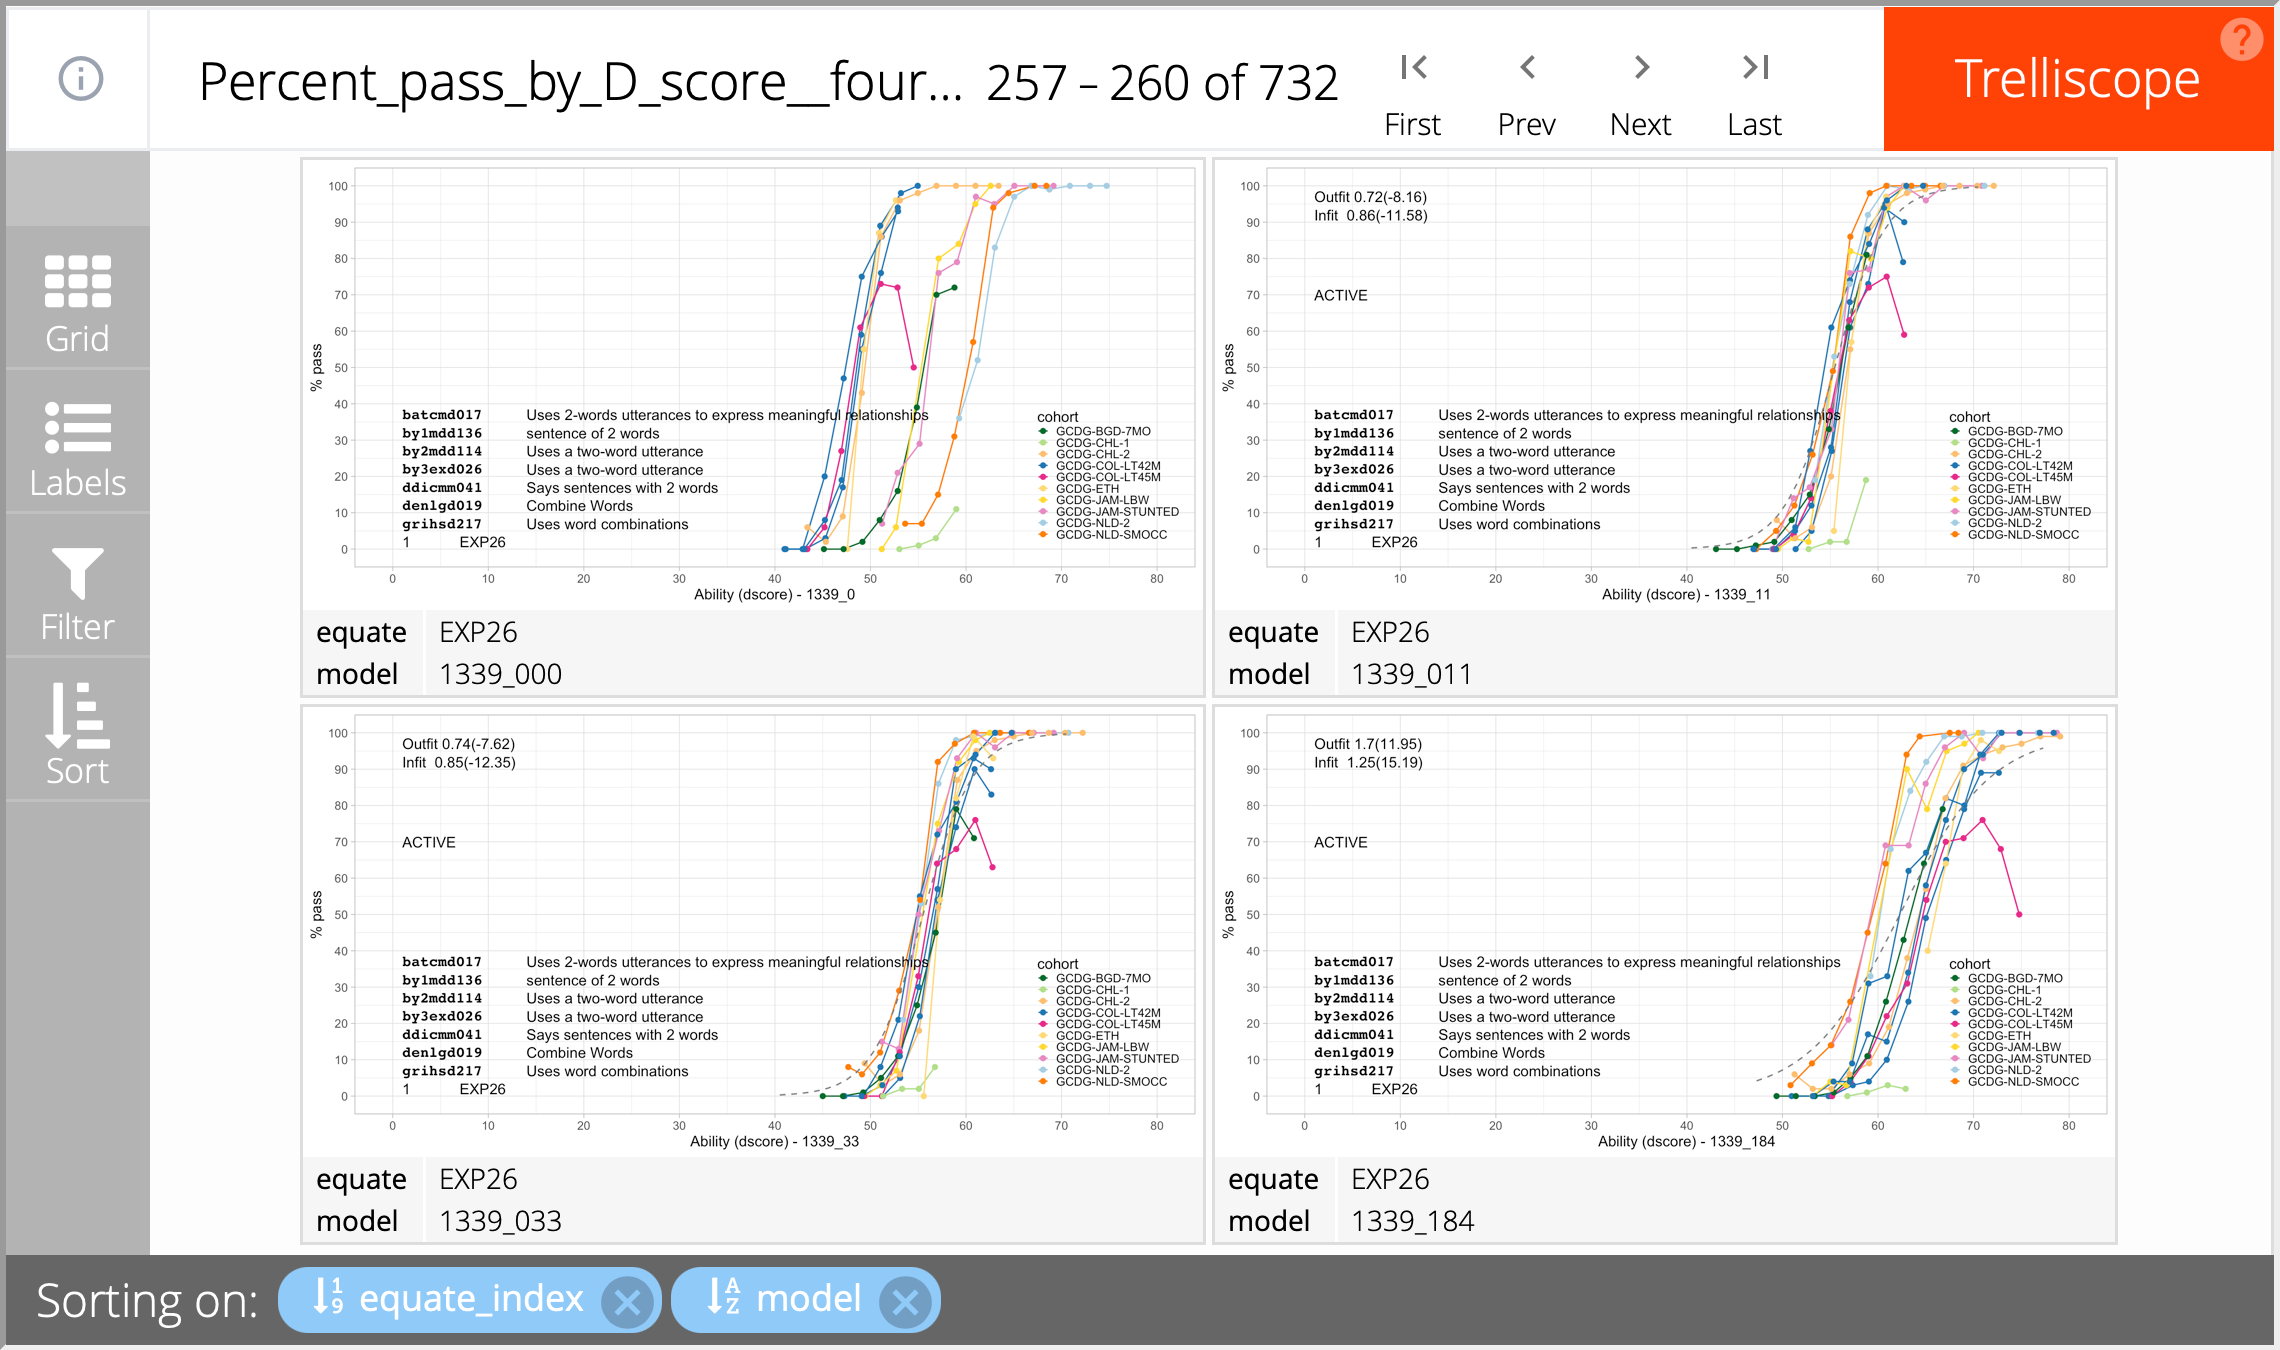
\includegraphics[width=1\linewidth]{fig/fig_5.4} 

}

\caption{\href{https://d-score.org/dbook-apps/p-d-equate-1339/\#display=Percent_pass_by_D_score__four_models\&nrow=2\&ncol=2\&arr=row\&pg=65\&labels=equate,model\&sort=equate_index;asc,model;asc\&filter=\&sidebar=\&fv=}{Percentage of children that pass similar milestones given their D-score as calculated under four models (1339 items, and 0, 11, 33 and 184 equate groups, respectively} (\url{https://d-score.org/dbook-apps/p-d-equate-1339/}).}\label{fig:p-d-equate-1339}
\end{figure}



Figure \ref{fig:p-d-equate-1339} shows how the passing percentage depends on the child's D-score as calculated under four models. All models include the same 1339 milestones, but differ in the number of active equates. The grey curve corresponds to the estimate made under the assumption that milestones are equally difficult. Good milestones for bridging instruments will have a tight bundle of curves. For example, equate \texttt{EXP26} has tight bundles especially in models \texttt{1339\_11} and \texttt{1339\_33}. By comparison, the curves of the two extreme models vary considerably: the model without any bridges (\texttt{1339\_0}) or the model with all bridges (\texttt{1339\_184}) are thus less than ideal. The shallow grey curve of model \texttt{1339\_184} indicates a poorer overall fit.

Outfit and infit statistics measure the residual deviation of the items to the grey curve. High values (e.g.~above 1.4) are undesirable and indicate lack of fit to the model. For example, the fit statistics for \texttt{EXP26} in model \texttt{1339\_184} (1.70 and 1.25) indicate a mediocre fit, whereas \texttt{EXP26} in models \texttt{1339\_33} and \texttt{1339\_11} fits well. Sometimes the individual item curves are steeper than the grey curve. This indicates that these milestones are more discriminative than the combined item. Model \texttt{1339\_0} lacks a grey curve and has no fit statistics for equate groups, because in that model, the combined item is not activated.

The probability curves provide a quick visual method for spotting promising and problematic equate groups. Examples of promising equate groups include \texttt{COG36}, \texttt{FM31}, \texttt{GM26} and \texttt{GM42}. A little more weak are \texttt{FM26} (has more variability), \texttt{FM52} (looks promising, but has a problem with the item \texttt{grigcd402} from the \texttt{GCDG\_JAM\_STUNTED} cohort), and \texttt{GM35} (does not align cohort \texttt{GCDG-ZAF}). In such cases, one may wish to move an item out of an equate group, combine equate groups, or inactivate troublesome links.

Until now we only looked at models that include all 1339 items. In practice, we may improve upon the model by selecting the subset of milestones that fit the Rasch model. The next section looks in this modelling step in more detail.

\hypertarget{sec:milestoneselection}{%
\section{Milestone selection}\label{sec:milestoneselection}}

\begin{figure}

{\centering 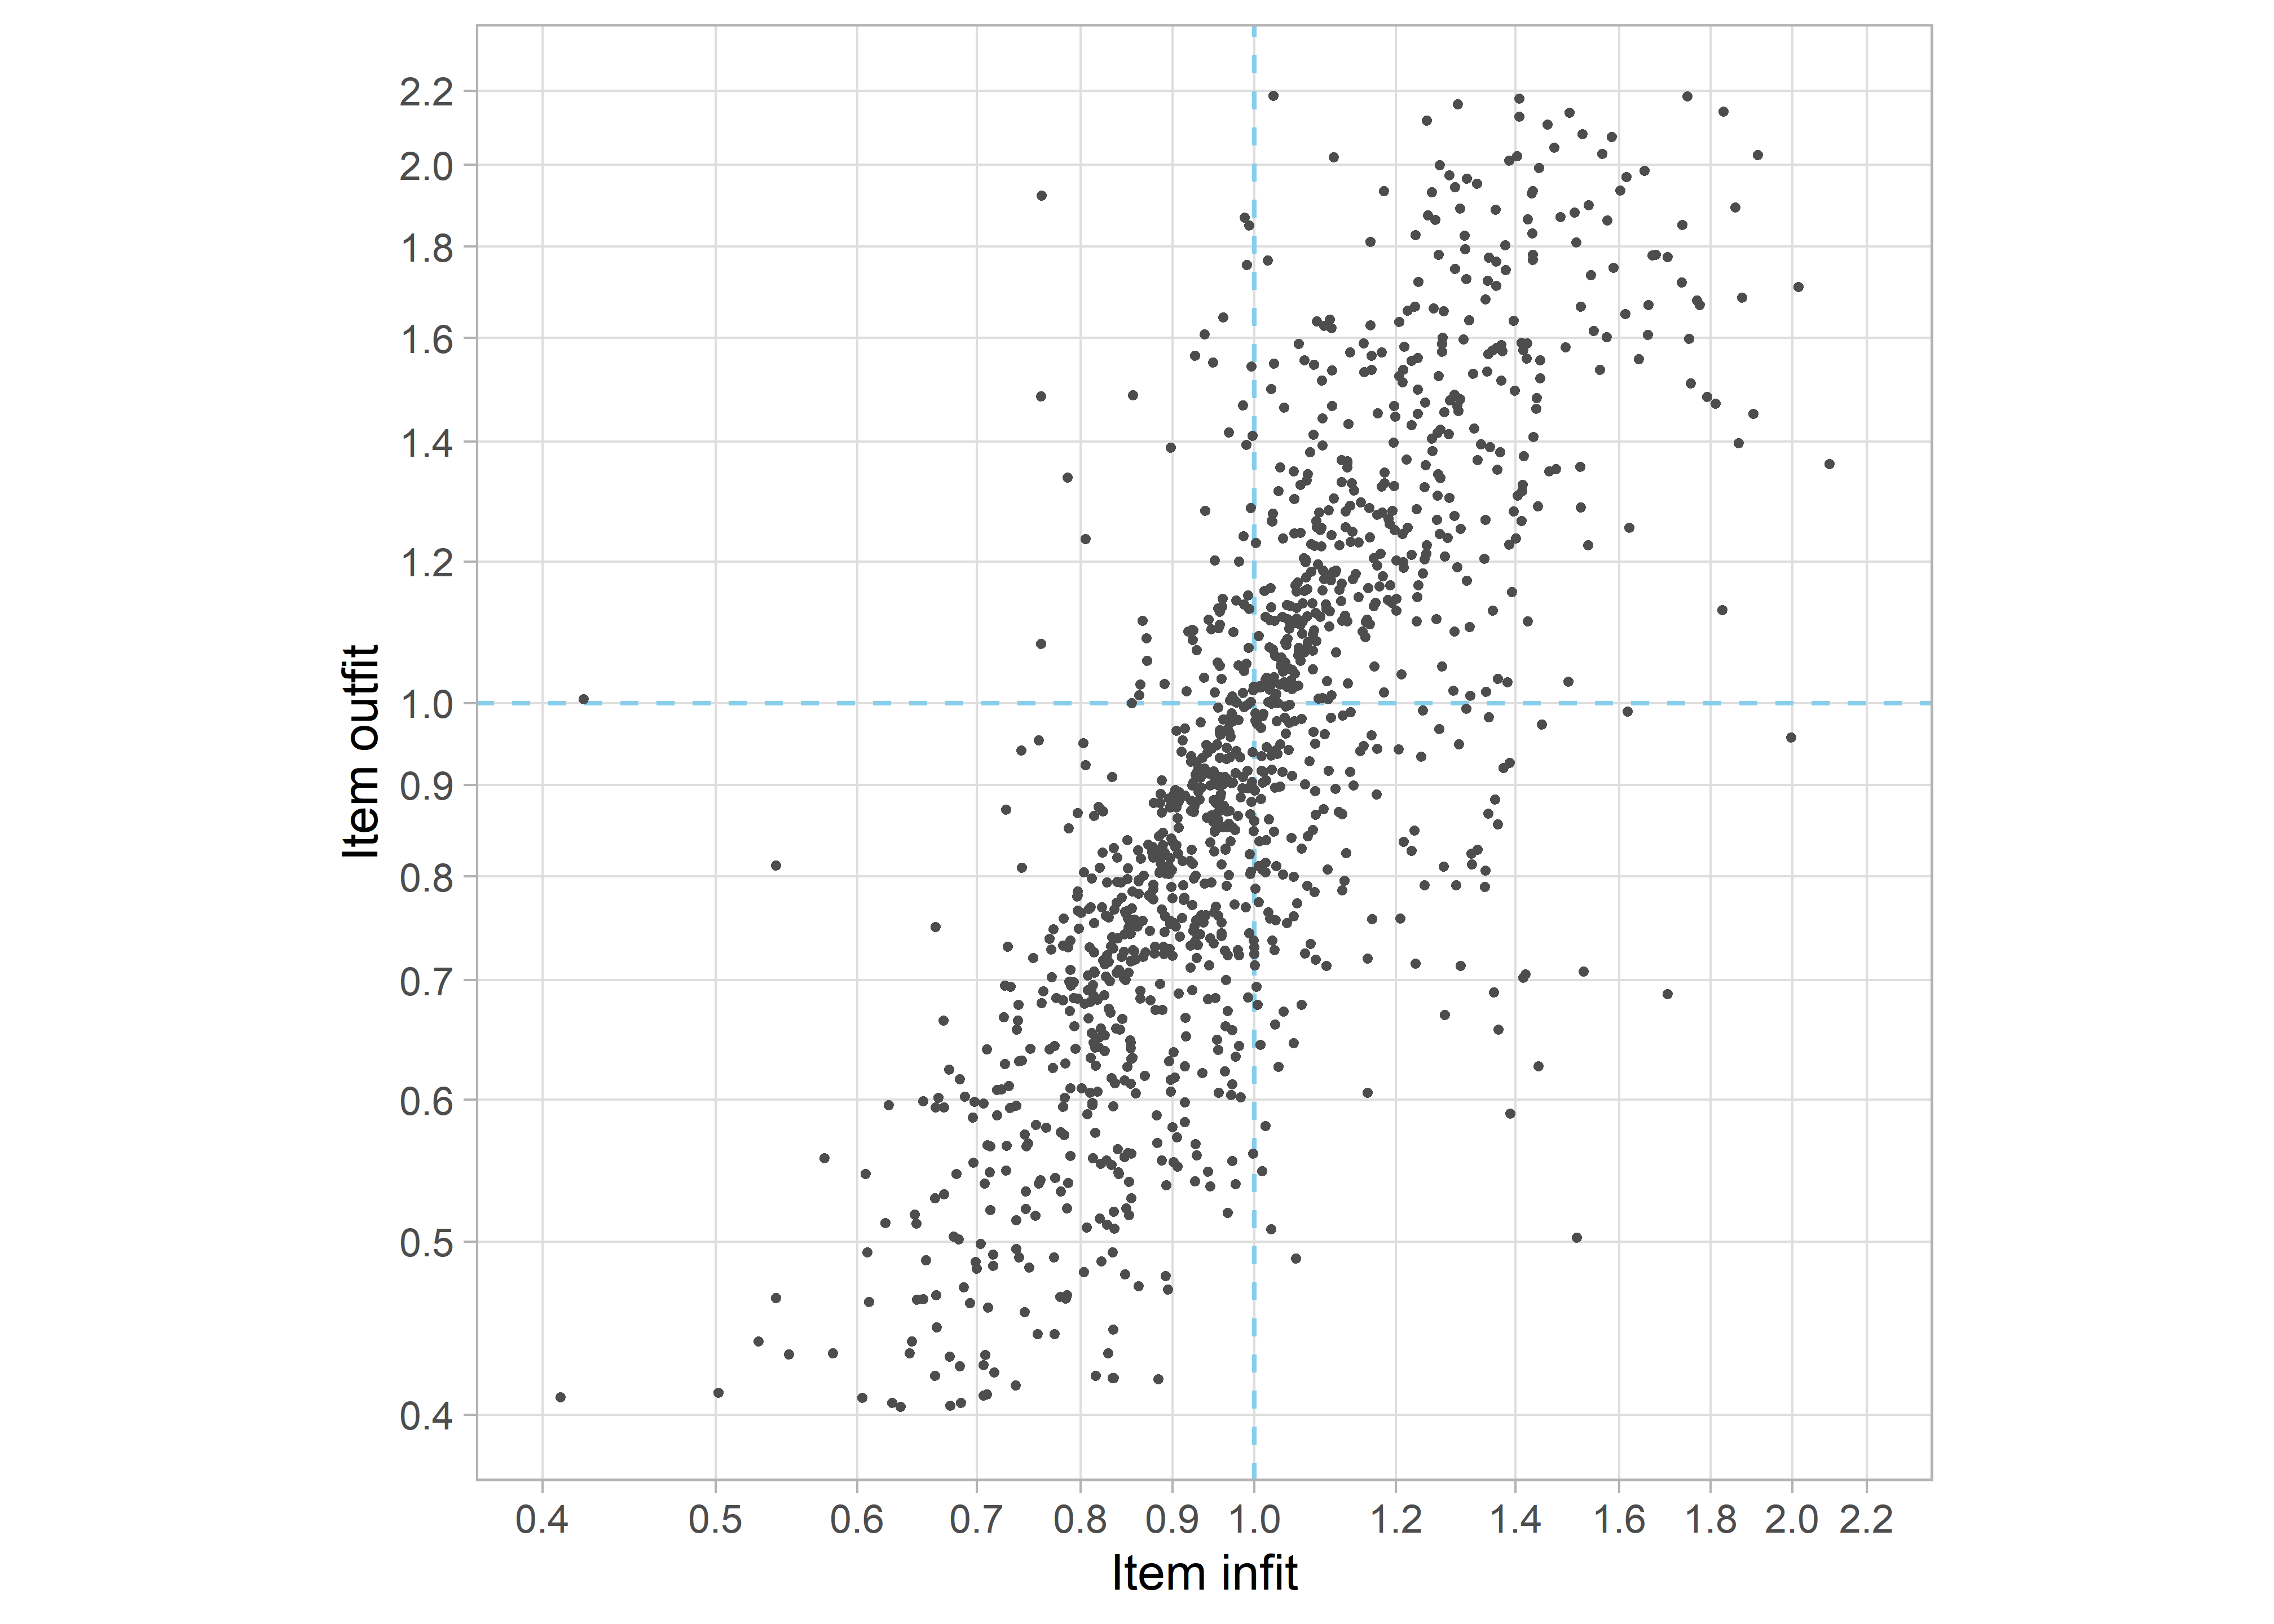
\includegraphics[width=0.75\linewidth]{dbook2_files/figure-latex/itemfit-1} 

}

\caption{Infit and outfit of 1339 items in model \texttt{1339\_11}. About 8 percent of the points falls outside the plot.}\label{fig:itemfit}
\end{figure}



Item infit and outfit are convenient statistics for selecting the milestones that fit the model. Figure \ref{fig:itemfit} displays the infit and outfit statistics of model \texttt{1339\_11}. The correlation between infit and outfit is high (\(r = 0.84\)). The expected value of the infit and outfit statistics for a perfect fit is 1.0. The centre of infit and outfit in Figure \ref{fig:itemfit} is approximately 1.0, so on average one could say the items fit the model. Note however that fit values above and below the values of 1.0 are qualitatively different. Item with fit statistics exceeding 1.0 fit the model less well than expected (\textbf{underfit}), whereas items with fit statistics lower than 1.0 fit the model better than expected (\textbf{overfit}). See \href{https://d-score.org/dbook1/sec-itemfit.html}{Booklet 1: Section 6.1} for more details.

Some practitioners remove both underfitting and overfitting items. However, we like to preserve overfitting items and be more strict in removing items that underfit. The idea is that preservation of the best fitting items may increase scale length, and hence reliability and measurement precision. Figure \ref{fig:itemfit} draws two cut-off lines at 1.0. Taking items with infit \textless{} 1.0 and outfit \textless{} 1.0 will select \textbf{631 out of 1339} items for further modelling.

A practical problem of item removal is that it also affects equate group composition. By default, a removed item will also be removed from the equate group, so item removal may reduce the size of an equate group below two items. For passive equates this is no problem, since passive equates do no affect the estimates. However, removal of an underfitting item from an active equate group will break the bridge between the instrument it pertains to and the rest of the item set. Potentially this can result in substantial effects on the D-score distribution of the cohort, as demonstrated in Figure \ref{fig:model1339}. As a solution, we force any items that are members of active equate groups to remain in the analysis. If that leads to substantially worse equate fit in the next model, we must search for alternative equate groups that bridge the same instruments and that are less sensitive to misfit.

\hypertarget{sec:othermodelling}{%
\section{Other modelling actions}\label{sec:othermodelling}}

\hypertarget{instrument-fit}{%
\subsection{Instrument fit}\label{instrument-fit}}

\begin{figure}

{\centering 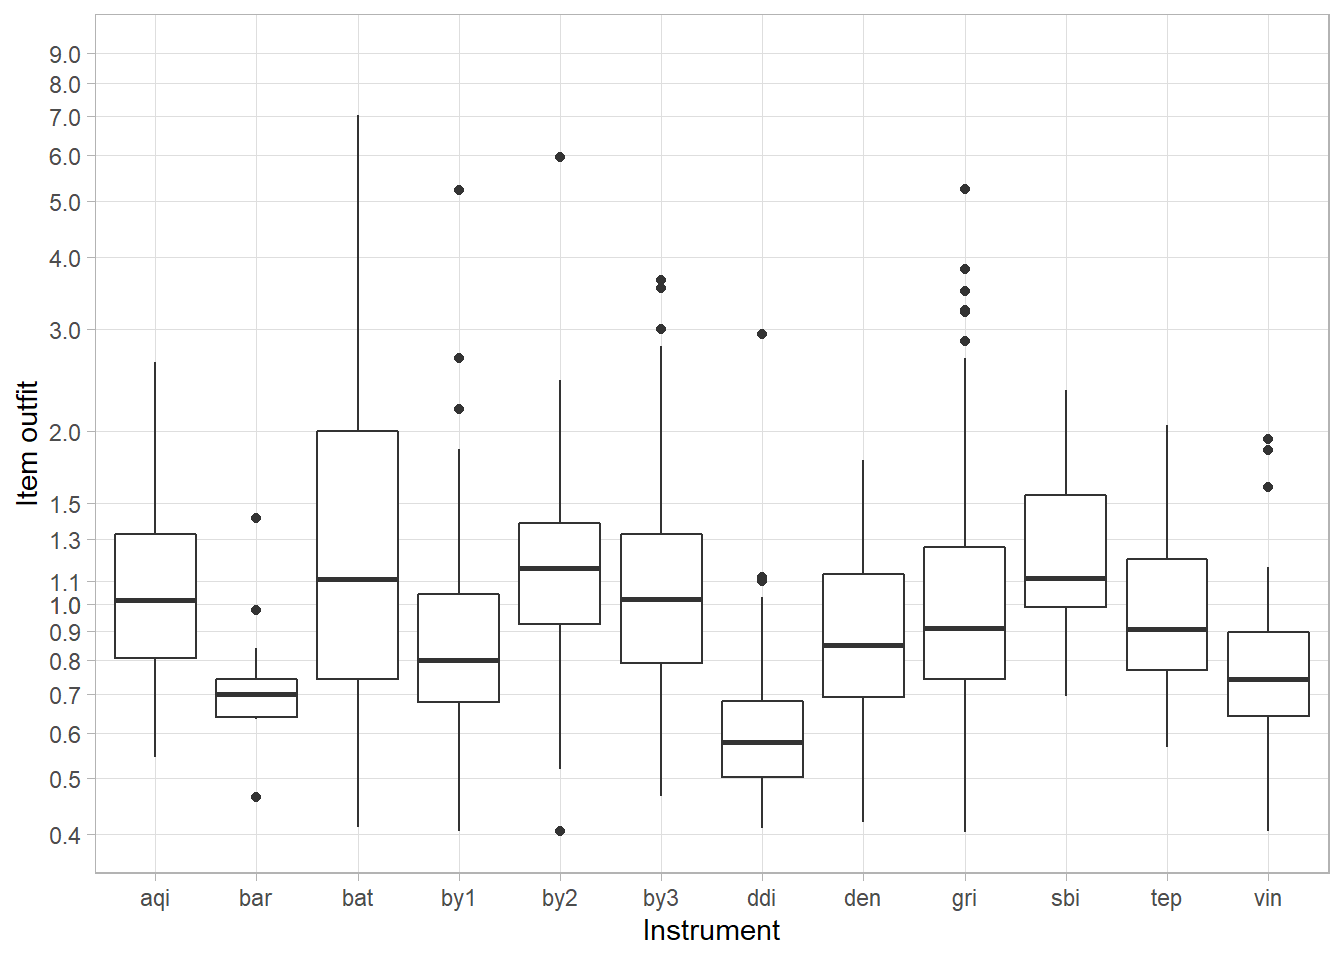
\includegraphics[width=1\linewidth]{dbook2_files/figure-latex/itembox-1} 

}

\caption{Box plot of the distribution of item outfit per instrument in model \texttt{1339\_11}.}\label{fig:itembox}
\end{figure}



Some instruments fit better than others. Figure \ref{fig:itembox} shows the box plots of outfit per instrument. Instruments \texttt{bar}, \texttt{by1}, \texttt{ddi} and \texttt{vin} generally fit well, whereas discrepancies between model and data are larger for \texttt{bat}, \texttt{by2} and \texttt{sbi}. Through additional modelling, we found that it was extremely difficult to get enough high-quality bridge items that could link \texttt{bat} (Battelle Development Inventory) to the other instruments. We also found that models without the Battelle were able to better discriminate children in the upper range of the D-score scale. We therefore opted to remove \texttt{bat} from the model, even though this meant that one cohort (\texttt{GCDG-BRA-2}) had to be dropped from the analysis.

It is not clear why \texttt{bat} does not fit. Perhaps the scoring system of the Battelle in three categories invokes scoring behaviour that is different from the PASS/FAIL scoring used by most other instruments, even though this appears to be less of a troublesome aspect in \texttt{aqi}, which also uses three response categories.

\hypertarget{splitting-combining-and-selecting-equate-groups}{%
\subsection{Splitting, combining and selecting equate groups}\label{splitting-combining-and-selecting-equate-groups}}

Most of the modelling effort went into finding a set of high-quality equate groups that link the instruments. For example, we tried to bridge the South-African study placing \texttt{vinxxc016} (uses a short sentence) into \texttt{EXP26} (two-word sentences) and \texttt{EXP36} (sentences of 3 or more words), but neither option led to a reasonable model. On the surface, milestone \texttt{by3gmd060} (balances on right foot, 2 seconds) appears to fit within \texttt{GM60} (balances on foot), but the analysis showed large discrepancies with the other items in the groups, so it had to be taken out.

Subject-matter experts identified 38 items that were thought to be cross-culturally incompatible. Table \ref{tab:crosscultural} provides an overview. Many of such milestones involve a specific language concept (such as a pronoun), refer to stairs (less common in rural settings), help in house or clothing behaviour. These items have different meanings in different contexts, so they were not used to bridge instruments.

\begin{table}

\caption{\label{tab:crosscultural}Milestones not used for equating because of limited cross-cultural validity}
\centering
\begin{tabular}[t]{>{}ll}
\toprule
Item & Label\\
\midrule
\ttfamily{aqislc023} & When you dress your baby does she lift her foot for her shoe, sock, or pant leg?\\
\ttfamily{aqislc041} & Using these exact words, ask your child, "Are you a girl or a boy?" Does your child answer correctly?\\
\ttfamily{by1mdd050} & Washes and dries hands\\
\ttfamily{by1pdd053} & Bowel and bladder control\\
\ttfamily{by1pdd054} & manipulates table edge actively\\
\addlinespace
\ttfamily{by2pdd069} & Walsk up stairs with help\\
\ttfamily{by3cgd043} & Walks down stairs with help\\
\ttfamily{by3cgd052} & Walks down stairs with help\\
\ttfamily{by3gmd047} & Clear Box: Front\\
\ttfamily{by3gmd049} & Clear Box: Sides\\
\addlinespace
\ttfamily{by3gmd057} & Uses pronouns\\
\ttfamily{by3gmd058} & Walks Up Stairs Series: Both feet on each step, with support.\\
\ttfamily{by3red030} & Walks Down Stairs Series: Both feet on each step, with support\\
\ttfamily{by3exd030} & Walks Up Stairs Series: Both feet on each step, alone.\\
\ttfamily{barxxx016} & Walks Down Stairs Series: Both feet on each step, alone\\
\addlinespace
\ttfamily{barxxx020} & Understands pronouns (him, me, my, you, your)\\
\ttfamily{dengmd020} & Eats with spoon without help (M; can ask parents)\\
\ttfamily{densld012} & Takes off shoes and socks (M; can ask parents)\\
\ttfamily{densld013} & Can dress (one piece) (M; can ask parents)\\
\ttfamily{grigmd219} & Walk Up Stairs\\
\addlinespace
\ttfamily{grigmd222} & Drink from a cup\\
\ttfamily{mdsgmd002} & help in house\\
\ttfamily{mdsgmd003} & (Locomotor) Walks up and down stairs.\\
\ttfamily{mdsgmd004} & (Locomotor) Goes alone on the stairs (any method)\\
\ttfamily{mdsgmd005} & Hands-and-knees crawling\\
\addlinespace
\ttfamily{mdsgmd006} & Standing with assistance\\
\ttfamily{ddifmm019} & Walking with assistance\\
\ttfamily{ddifmd154} & Standing alone\\
\ttfamily{vinxxc002} & Walking alone\\
\ttfamily{vinxxc003} & chew solid foods\\
\addlinespace
\ttfamily{vinxxc009} & take off socks / shoes\\
\ttfamily{vinxxc012} & get on with other children\\
\ttfamily{vinxxc014} & know what's edible\\
\ttfamily{vinxxc022} & walk upstairs\\
\ttfamily{vinxxc028} & avoid simple danger - knife / hot\\
\addlinespace
\ttfamily{vinxxc031} & help around the house / clear table\\
\ttfamily{vinxxc040} & Play or do things with other children of same age eg sing song\\
\ttfamily{ddifmm025} & Help with little things around the house eg pick up things\\
\bottomrule
\end{tabular}
\end{table}



\hypertarget{sec:iteminformation}{%
\section{Item information}\label{sec:iteminformation}}

Item information is a psychometric measure that quantifies the sensitivity of the item to changes in the person's ability. An item is most sensitive around the D-score value where the PASS probability equals the FAIL probability, which corresponds to the item difficulty (\(\delta_i\)). One unit change around \(\delta_i\) has a large effect on the probability of endorsing, while one unit change far away from \(\delta_i\) has negligible impact. Suppose person A had passing probability \(0.7\) for some item. The information delivered by that item for person A is the product \(0.7 \times (1.0 - 0.7) = 0.21\). Suppose person B has a D-score that coincides with the difficulty level of the item. In that case, the information for B equals \(0.5 \times (1 - 0.5) = 0.25\), the maximum. Likewise, for a person C with high ability, the information could be \(0.98 * 0.02 = 0.02\), so that item carries almost no information for person C.

The information is inversely related to the error of measurement. More information amounts to less measurement error. For each response in the data, we can compute the amount of information it contributed to the model D-score. By summing the information over persons, we obtain a measure of certainty about the difficulty estimate of the item. This sum of information incorporates both the number of administrations and the quality of the match between person abilities and item difficulty.

\begin{figure}

{\centering 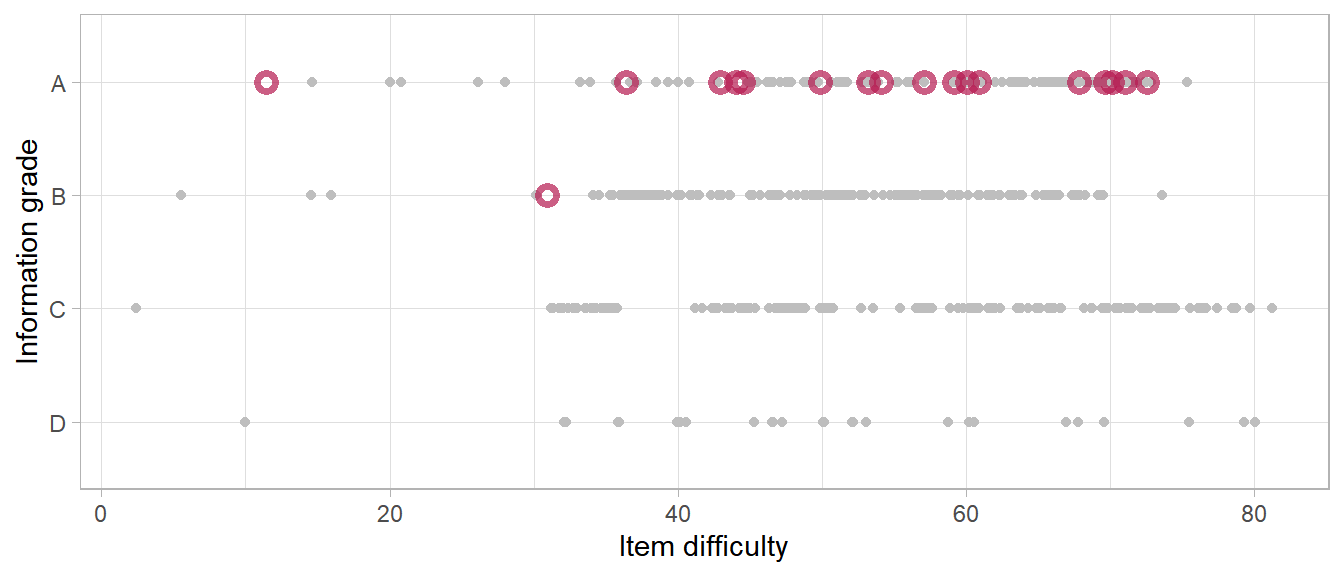
\includegraphics[width=1\linewidth]{dbook2_files/figure-latex/iteminfo-1} 

}

\caption{Item information grade by item difficulty for the final model}\label{fig:iteminfo}
\end{figure}



Figure \ref{fig:iteminfo} displays the summed information for each item, divided into four grades: A(best) to D (worst). The information grade measures the stability of the difficulty estimate. Most items receive grades higher than C. In total, 30 milestones have grade D. Adding these items to future studies may yield important additional information.

The red circles indicate active equate groups. Most have grade A, so we have a lot of information about the items that form the active equate groups. Table \ref{tab:equateinfo} displays more detailed information for the active equate groups. The sample sizes are reasonably large. Many information statistics are well is above 100; the criterion for Grade A. The interpretation of this criterion is as follows. Suppose that we obtain a sample of 400 persons who are all perfectly calibrated to the item of interest. In that case, the information for that item will be equal to 100.

\begin{table}

\caption{\label{tab:equateinfo}Equate group information in the final model.}
\centering
\begin{tabular}[t]{lrrrl}
\toprule
Equate group & Difficulty & Sample Size & Information & Grade\\
\midrule
EXP2 & 11.4 & 3608 & 162.3 & A\\
REC6 & 30.9 & 5428 & 95.4 & B\\
GM25 & 36.4 & 6380 & 470.6 & A\\
FM26 & 42.9 & 4155 & 296.8 & A\\
GM35 & 44.0 & 5522 & 356.0 & A\\
\addlinespace
COG36 & 44.5 & 7912 & 230.0 & A\\
GM42 & 49.9 & 5953 & 327.7 & A\\
FM31 & 53.2 & 10991 & 731.7 & A\\
COG55 & 54.1 & 5647 & 420.3 & A\\
FM72 & 57.1 & 5430 & 253.6 & A\\
\addlinespace
EXP26 & 59.1 & 9119 & 578.8 & A\\
SA1 & 60.1 & 3363 & 172.1 & A\\
FM38 & 60.9 & 10236 & 491.7 & A\\
FM52 & 67.8 & 13487 & 1159.9 & A\\
FM43 & 69.7 & 15765 & 1563.9 & A\\
\addlinespace
GM60 & 70.1 & 9519 & 1070.6 & A\\
REC40 & 71.0 & 10393 & 1182.9 & A\\
FM61 & 72.6 & 10612 & 945.9 & A\\
\bottomrule
\end{tabular}
\end{table}

\hypertarget{sec:finalmodel}{%
\section{Final model}\label{sec:finalmodel}}

Unfortunately, there is no single index of model fit that we can optimise. Modelling is more like a balancing act among multiple competing objectives, such as

\begin{itemize}
\tightlist
\item
  preserving as many items as possible that fit the model;
\item
  finding high-quality active equate groups that span many cohorts and instruments;
\item
  picking active equate groups for which we have enough information;
\item
  providing reasonable age-conditional distributions of the D-score;
\item
  representing various developmental domains in a fair way;
\item
  preserving well-fitting historical models as new data become available;
\item
  maintaining a reasonable calculation time.
\end{itemize}

This chapter showed various modelling techniques and ways to assess the validity of the model. In real life, we fitted a total number of 140 models on the data and made many choices that weigh the above objectives. The final model for the GCDG data consists of 565 items (originating from 14 instruments) that fit the Rasch model and that connect through 18 equate groups. Due to the sparseness of data at the very young ages, the quality of the model is best for ages between 4-36 months.

Model \texttt{565\_18} formed the basis of the publication by \protect\hyperlink{ref-Weber2019}{Weber et al.} (\protect\hyperlink{ref-Weber2019}{2019}). Additional detail on model \texttt{565\_18} is available through the \href{https://tnochildhealthstatistics.shinyapps.io/dmodel/}{\texttt{dmodel} shiny app}.

\hypertarget{ch:ability}{%
\chapter{Comparing ability}\label{ch:ability}}

\begin{quote}
Author: Iris Eekhout, Stef van Buuren
\end{quote}

Once we identified a satisfactory D-score model, we may calculate the D-score for children from different cohorts and compare their values. This chapter highlights various techniques and issues for comparing D-score distributions between studies. We will address the following topics:

\begin{itemize}
\tightlist
\item
  Comparing child development across studies (\ref{sec:dscores})
\item
  Precision of the D-score (\ref{sec:sem})
\item
  Domain coverage (\ref{sec:domains})
\end{itemize}

\hypertarget{sec:dscores}{%
\section{Comparing child development across studies}\label{sec:dscores}}

\begin{figure}

{\centering 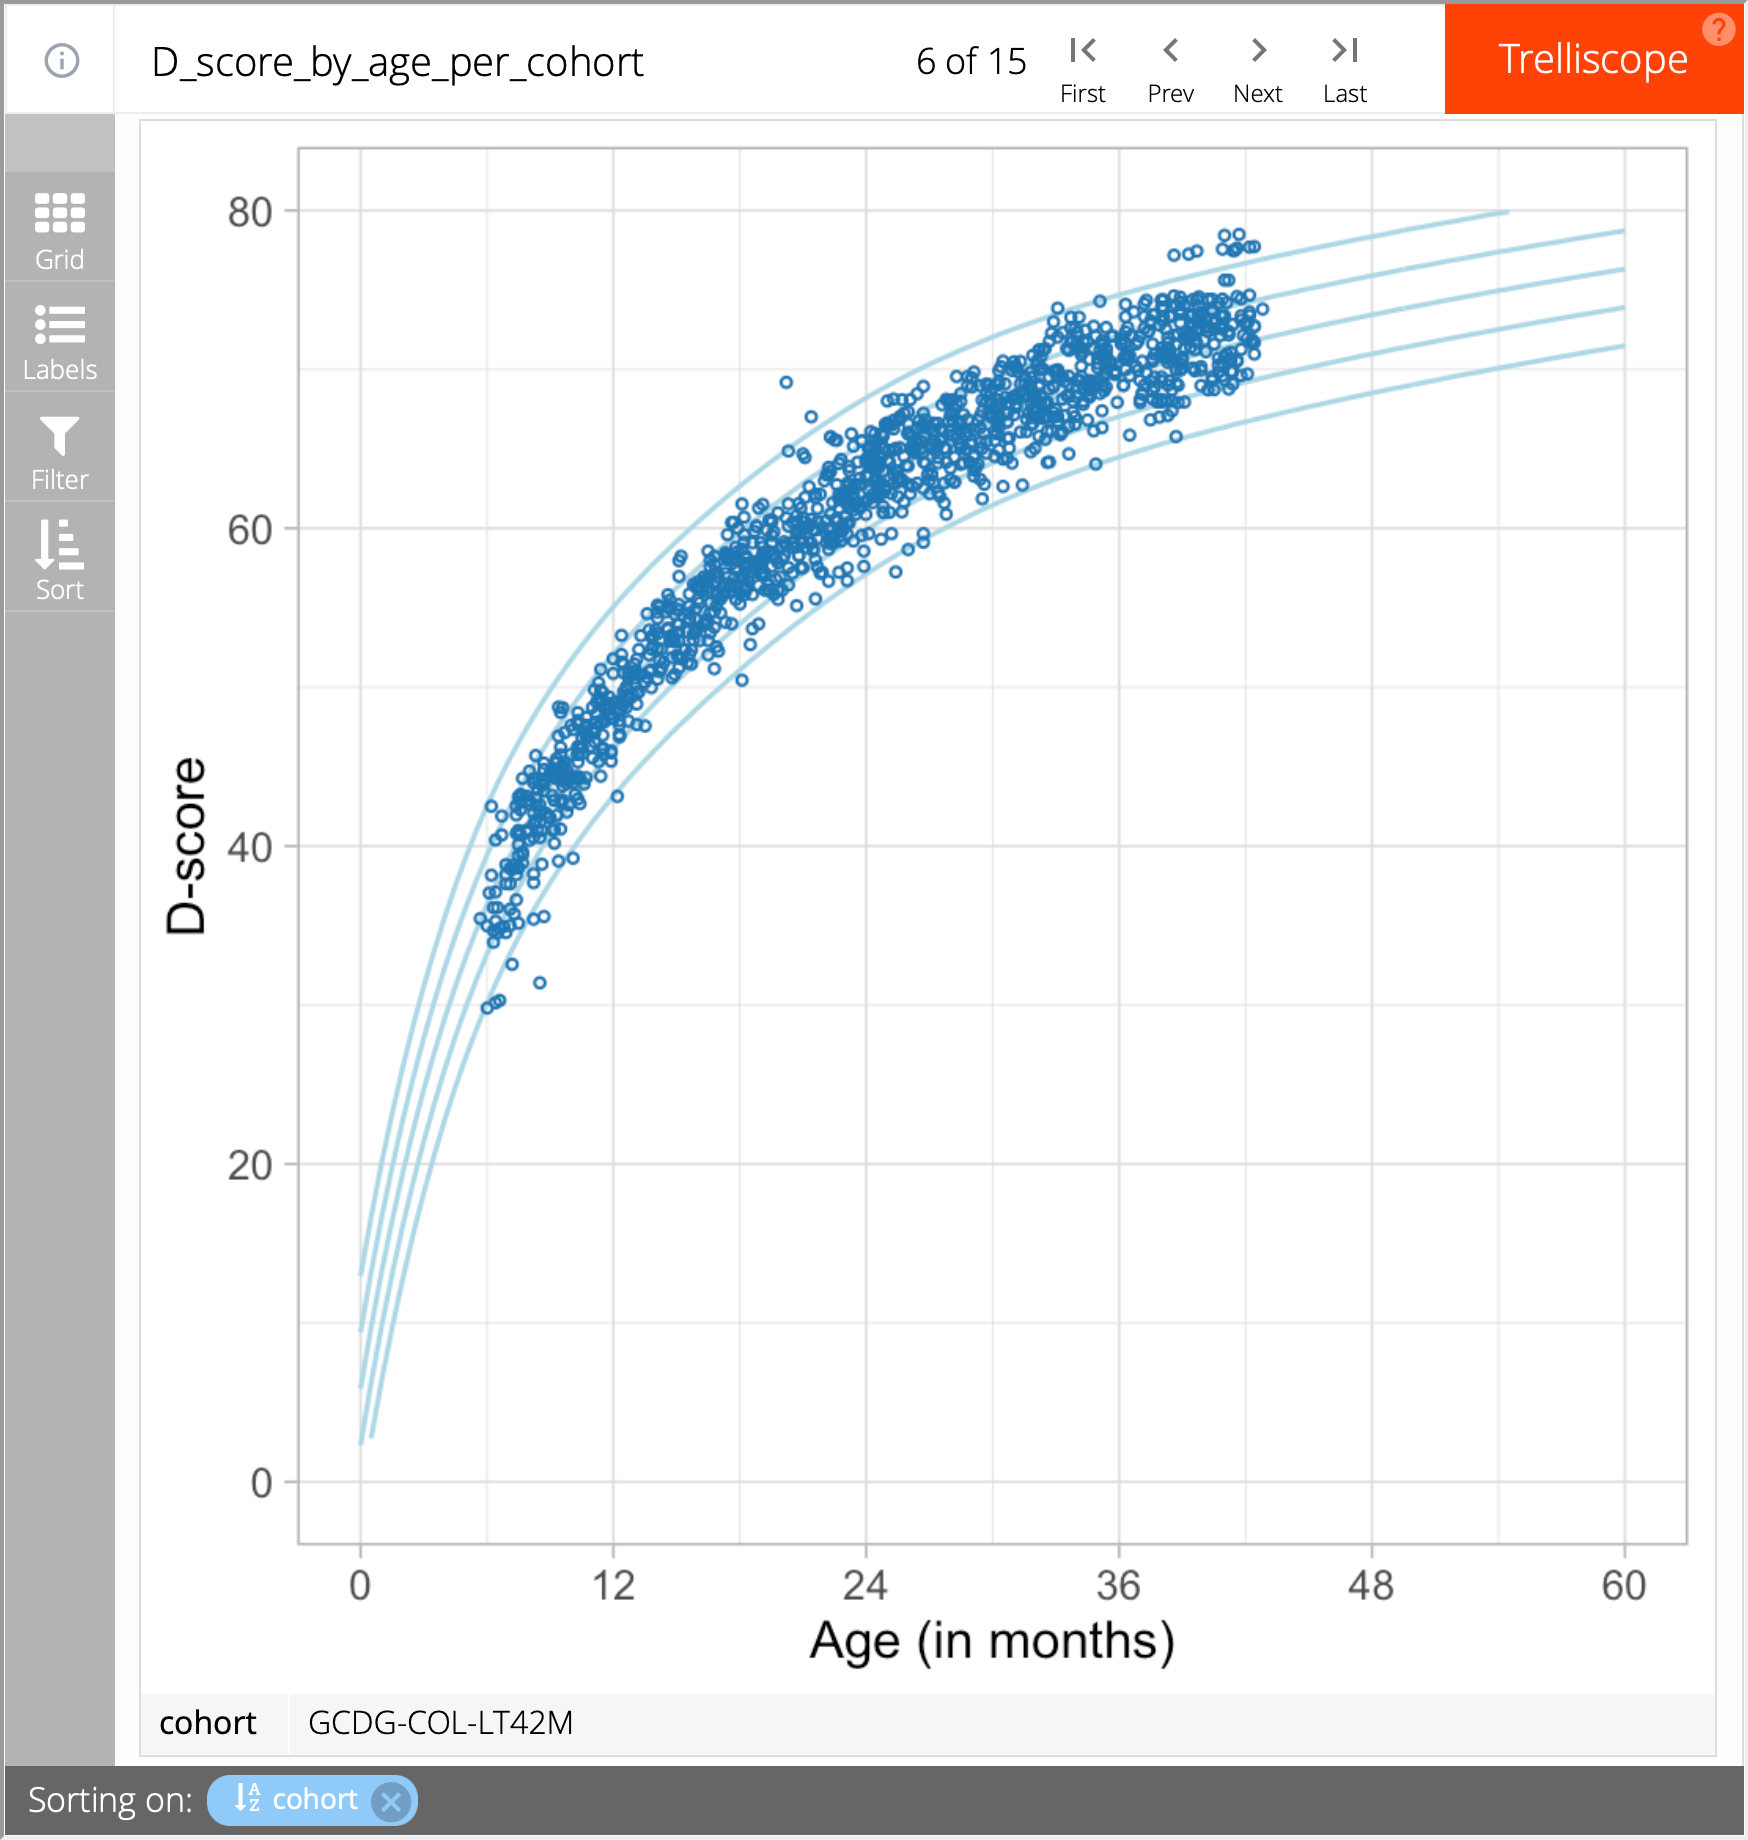
\includegraphics[width=1\linewidth]{fig/fig_6.1} 

}

\caption{\href{https://d-score.org/dbook-apps/gcdgdscores/\#display=by_cohort\&nrow=1\&ncol=1\&arr=row\&pg=6\&labels=cohort\&sort=cohort;asc\&filter=\&sidebar=\&fv=}{D-score distributions by study} (\url{https://d-score.org/dbook-apps/gcdgdscores/}).}\label{fig:dscoredist}
\end{figure}



Figure \ref{fig:dscoredist} shows the scatterplot of the D-score by age separately for each cohort. Remember from section \ref{sec:gcdgoverview} that each study selected its own set of instruments to collect the data. The scatterplots demonstrate a significant advance made possible by the D-score: We can plot the developmental scores of children from \textbf{different} cohorts, with \textbf{different} ages, using \textbf{different} instruments, on the \textbf{same} vertical axis.

The five blue lines guide the eye. These lines indicate the locations of the -2SD, -1SD, 0SD, +1SD and +2SD quantiles at each age in the combined data. \href{https://d-score.org/dbook1/sec-reference.html}{Section 5.4, booklet I} motivates the idea and provides some technical details. We'll come back to these lines in section \ref{sec:references}.

By and large, the data in every study follow the blue lines. Perhaps the most obvious exception is the \texttt{GCDG-JAM-STUNTED} cohort, where older children somewhat exceed the D-score range. It is unknown whether this is real, or due to a sub-optimal calibration of the instrument.

\begin{figure}

{\centering 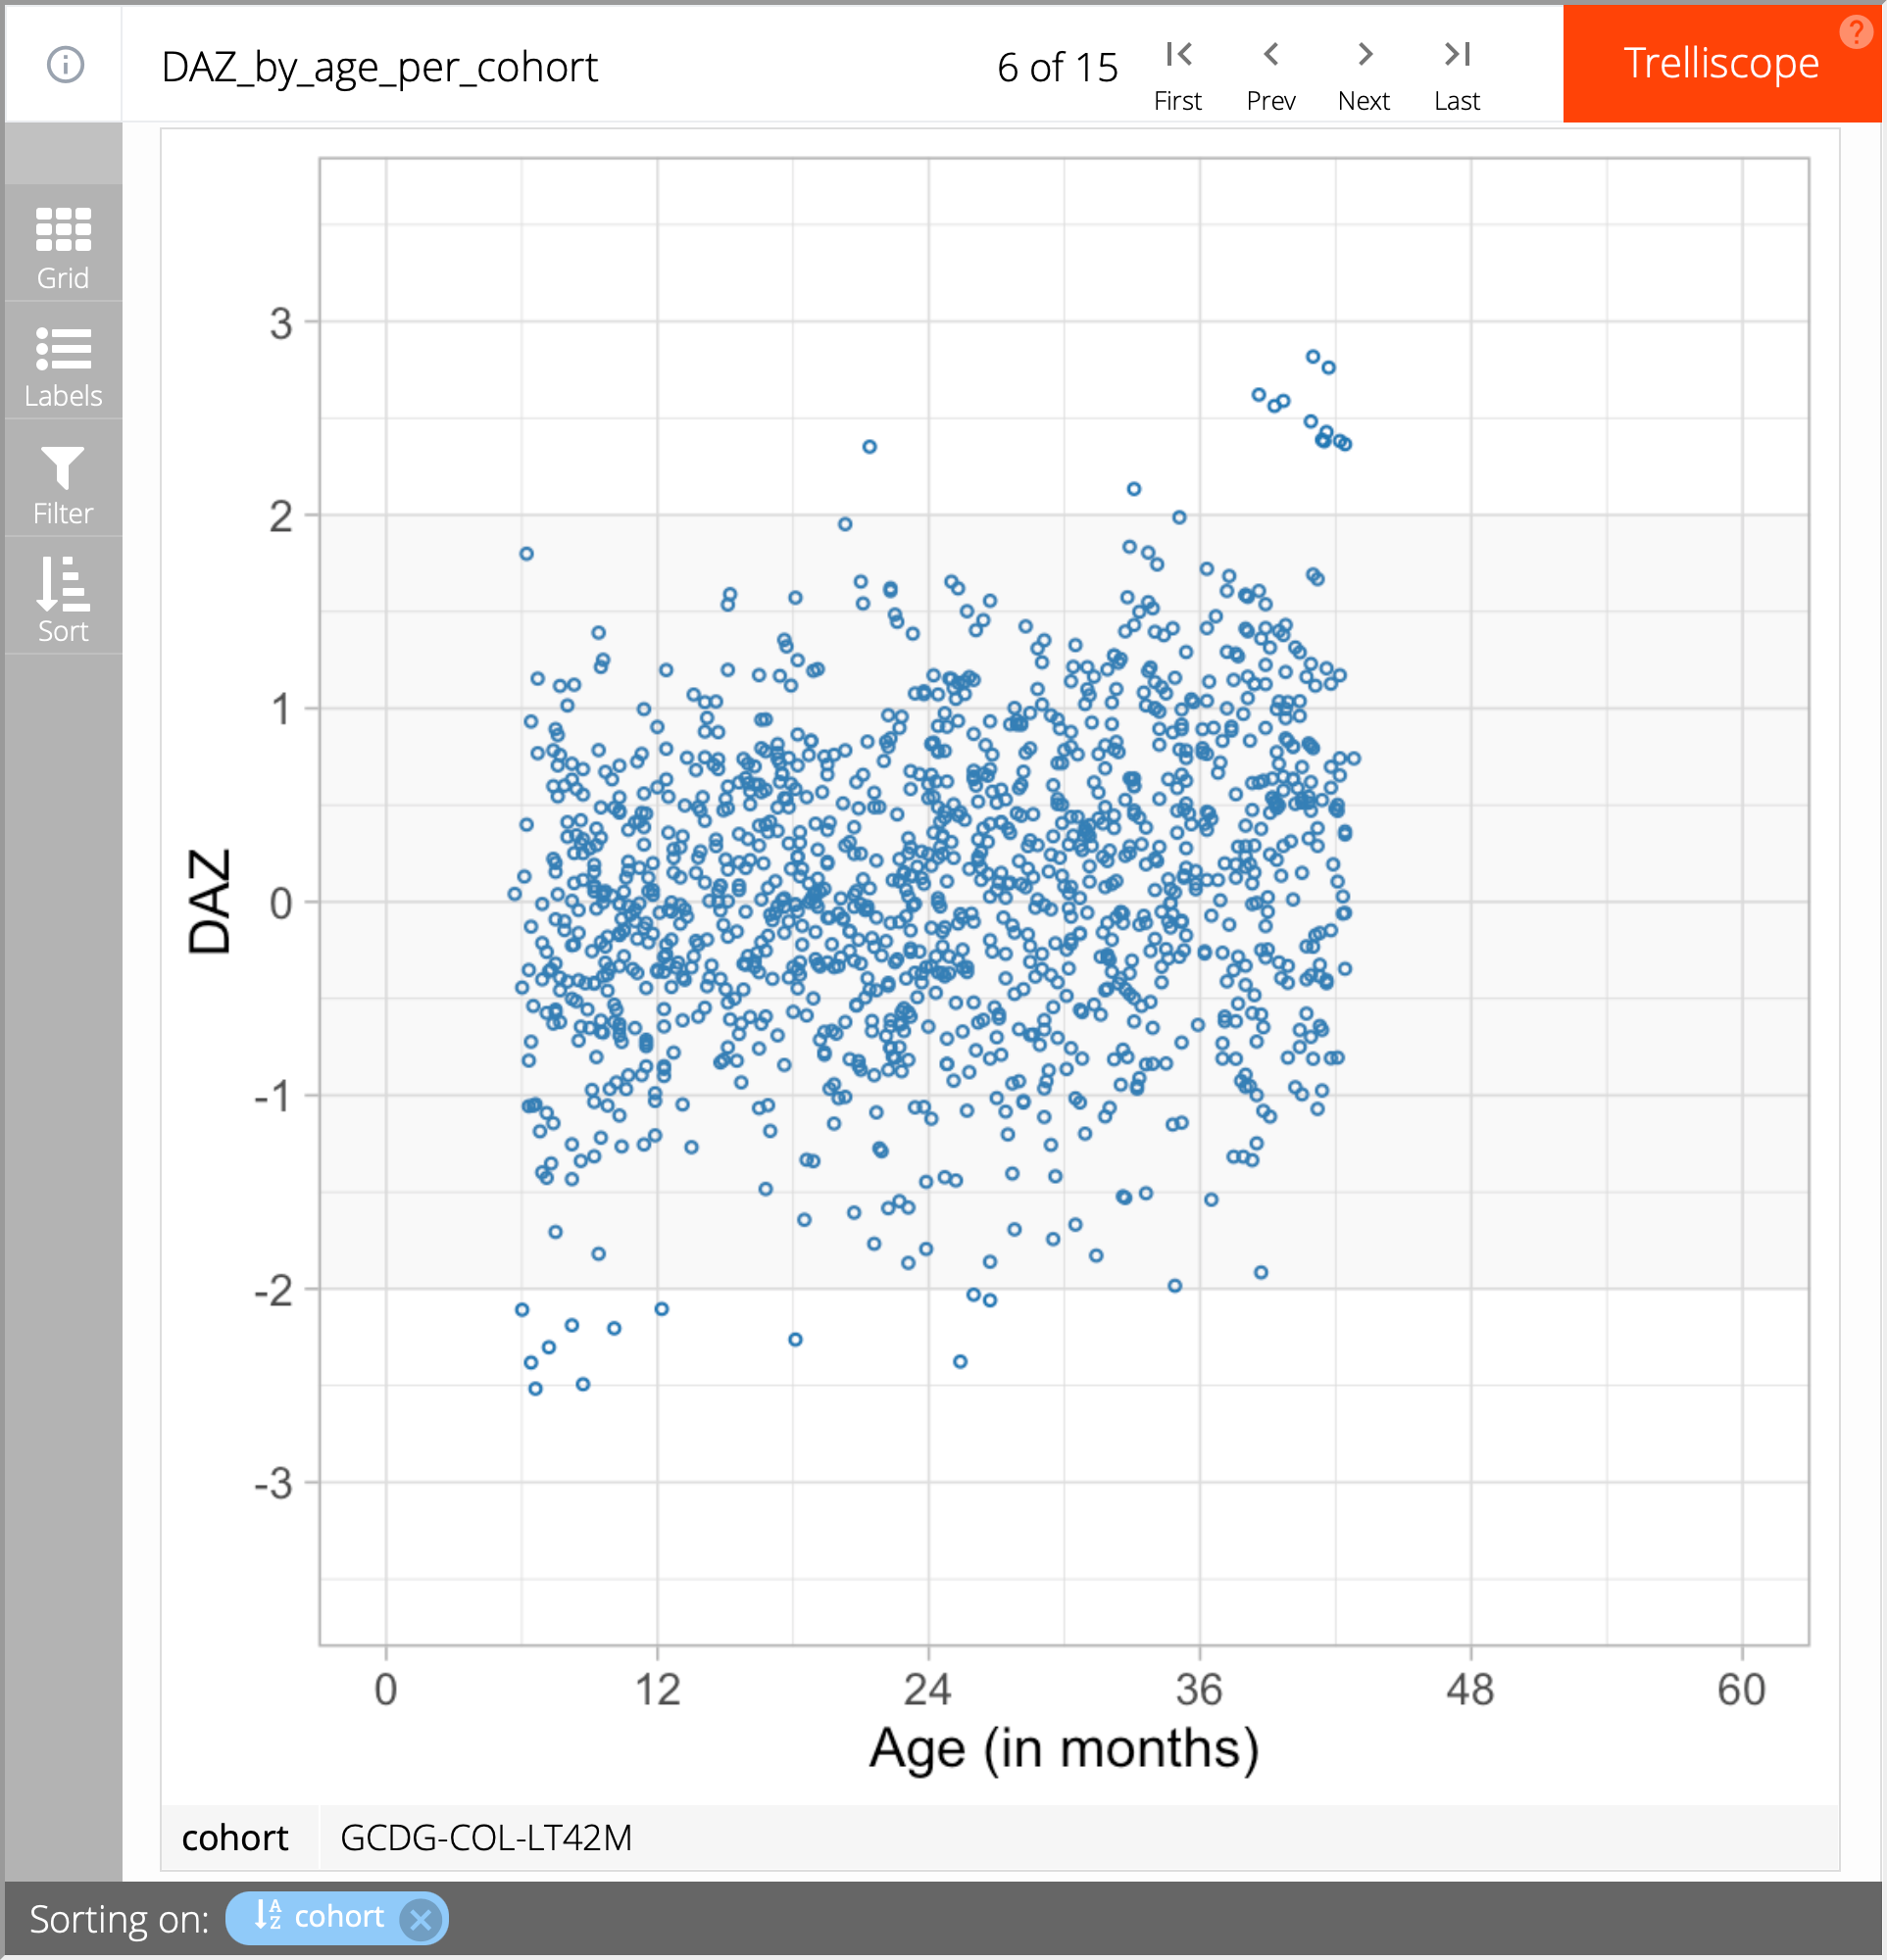
\includegraphics[width=1\linewidth]{fig/fig_6.1a} 

}

\caption{\href{https://d-score.org/dbook-apps/gcdgdaz/\#display=by_cohort\&nrow=1\&ncol=1\&arr=row\&pg=6\&labels=cohort\&sort=cohort;asc\&filter=\&sidebar=\&fv=}{DAZ distributions by study} (\url{https://d-score.org/dbook-apps/gcdgdaz/}).}\label{fig:dazdist}
\end{figure}



Figure \ref{fig:dazdist} plots the same data with D-score transformed into age standardized scores (DAZ). Replacing the D-score by the DAZ emphasises the differences both within and between studies. The majority of observations lies between the -2 SD and +2 SD lines in all cohorts. Using DAZ makes is easier to spot deviating trends, e.g., for the Jamaican or Ethiopian data.

\hypertarget{sec:sem}{%
\section{Precision of the D-score}\label{sec:sem}}

The \href{https://d-score.org/dbook1/sec-dscoreestimation.html\#eap-algorithm-numerical-example}{EAP algorithm} estimates the D-score from a set of PASS/FAIL scores. The standard deviation of the posterior distribution (or \emph{sem}: standard error of measurement) quantifies the imprecision of the D-score estimate. The \emph{sem} is inversely related to the number of items. Thus, when we administer more milestones, the \emph{sem} of the D-score drops.

\begin{figure}

{\centering 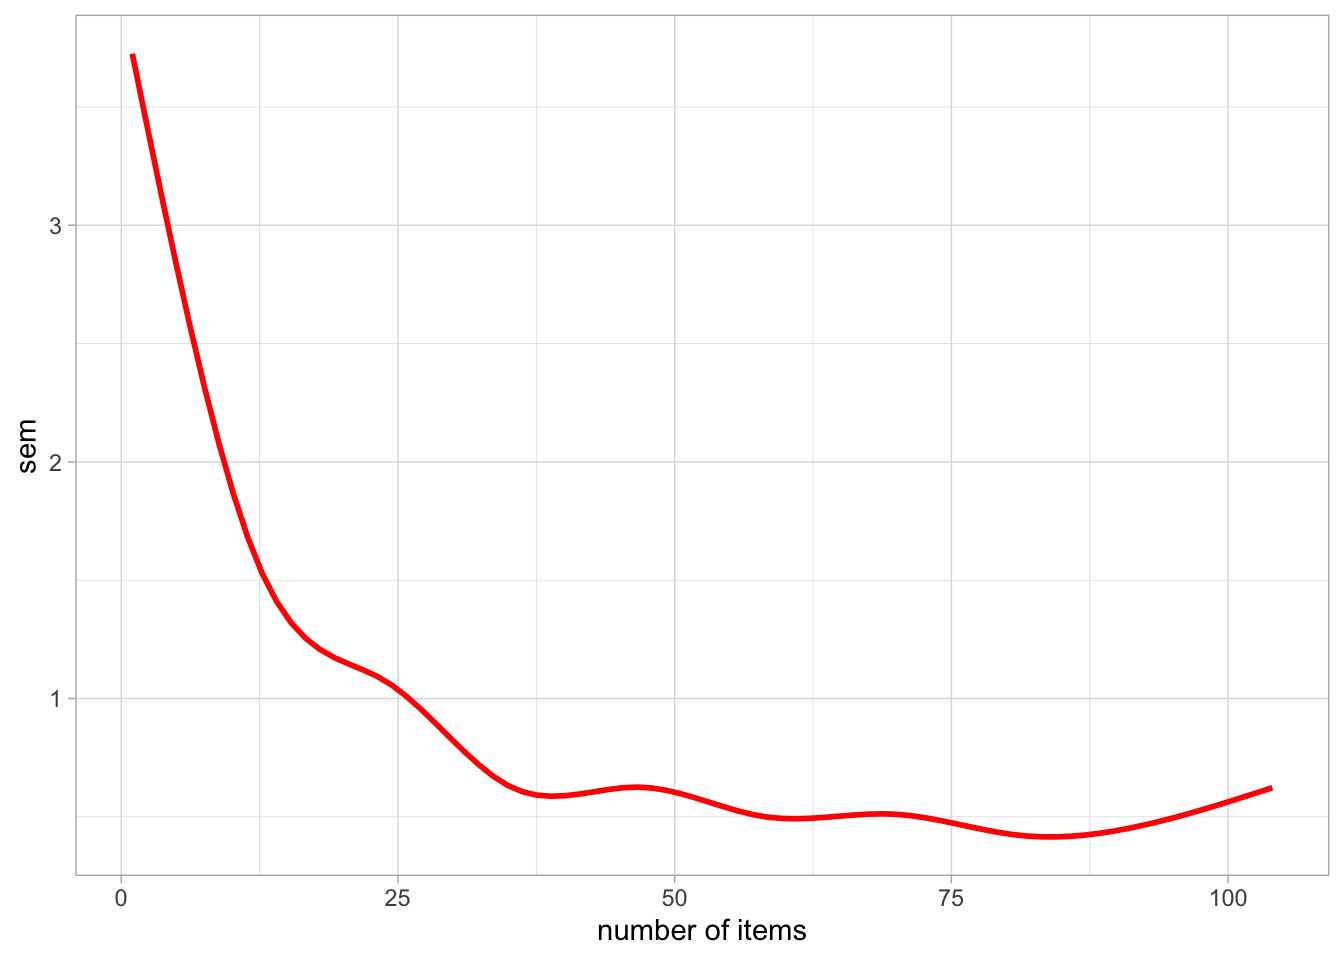
\includegraphics[width=1\linewidth]{dbook2_files/figure-latex/semforn-1} 

}

\caption{Standard error of measurement (\emph{sem}) as a function of the number of items.}\label{fig:semforn}
\end{figure}



Figure \ref{fig:semforn} shows that the \emph{sem} drops off rapidly when the number of items is low and stabilises after about 35 items. Apart from test length, the precision of the D-score also depends on item information (c.f. section \ref{sec:iteminformation}). Administering items that are too easy, or too difficult, does not improve precision. The figure suggests that - in practice - a single D-score cannot be more precise than 0.5 D-score units.

\begin{figure}

{\centering 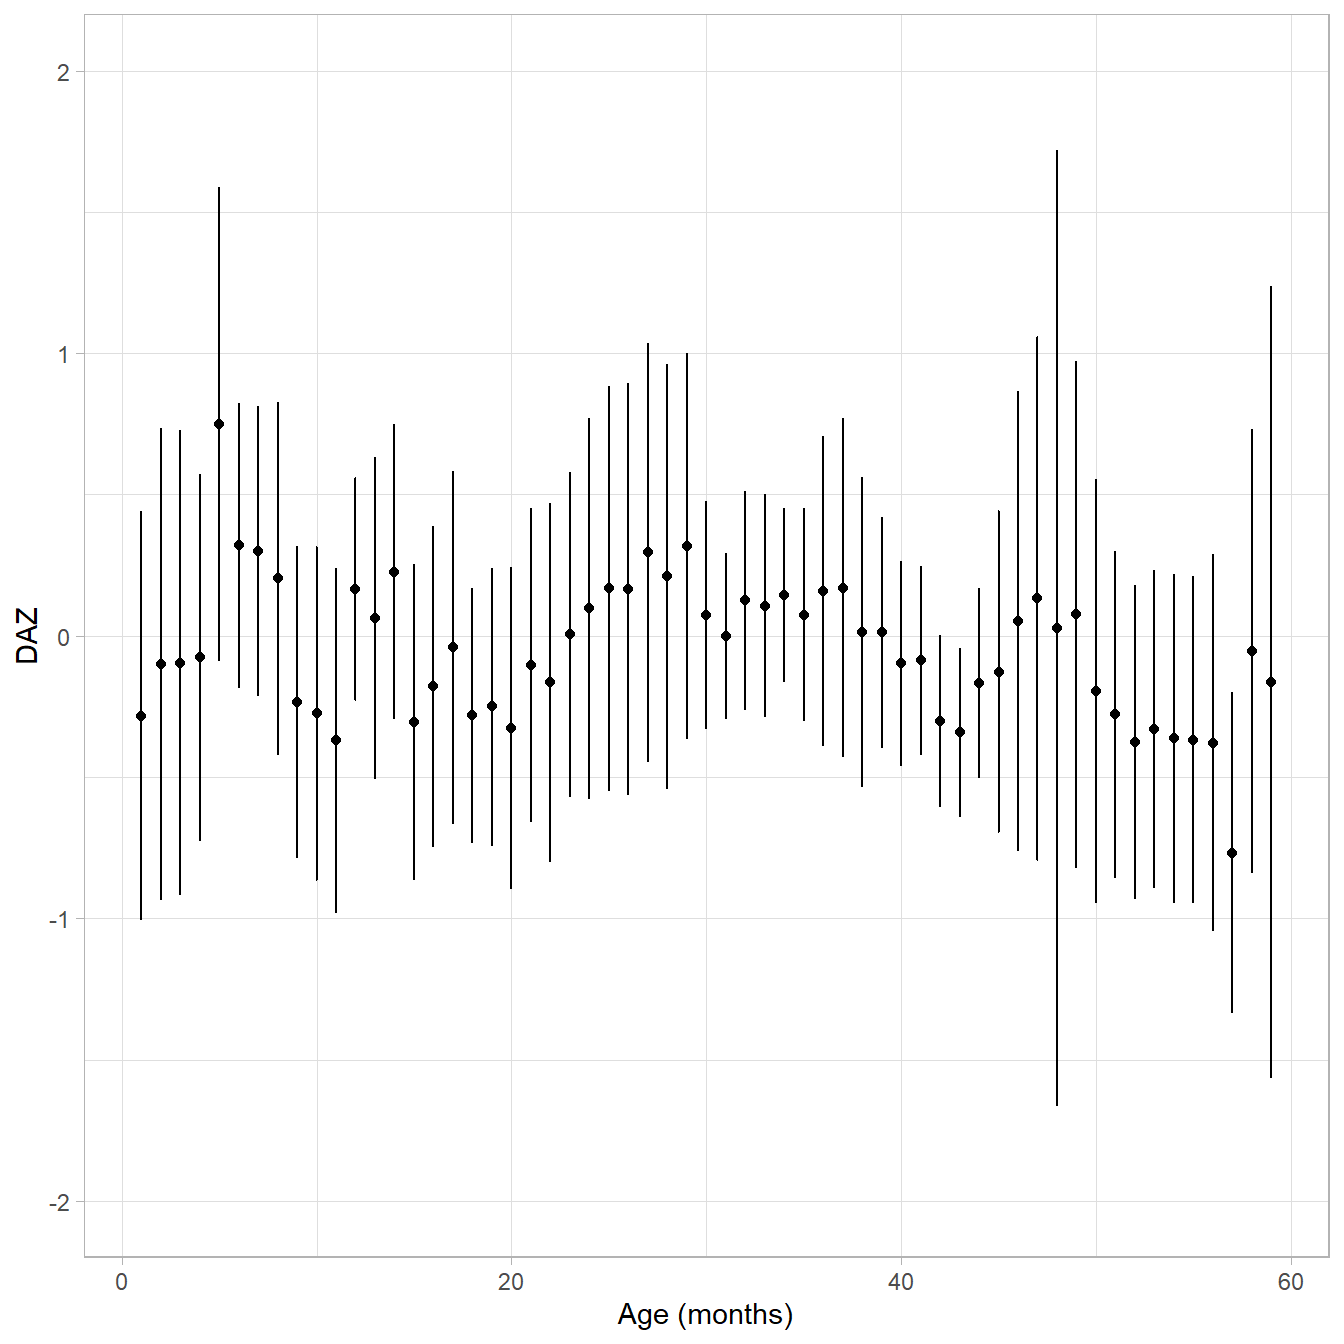
\includegraphics[width=1\linewidth]{dbook2_files/figure-latex/semfora-1} 

}

\caption{Mean DAZ \(\pm\) \emph{sem} as a function of age.}\label{fig:semfora}
\end{figure}



One may wonder whether the \emph{sem} depends on age. Figure \ref{fig:semfora} suggests that this is not the case. The average DAZ is close to zero everywhere, as expected. The interval DAZ \(\pm\) \emph{sem} will cover the true, but unknown, DAZ in about 68\% of the cases. While the interval varies somewhat across ages, there is no systematic age trend.

\begin{figure}

{\centering 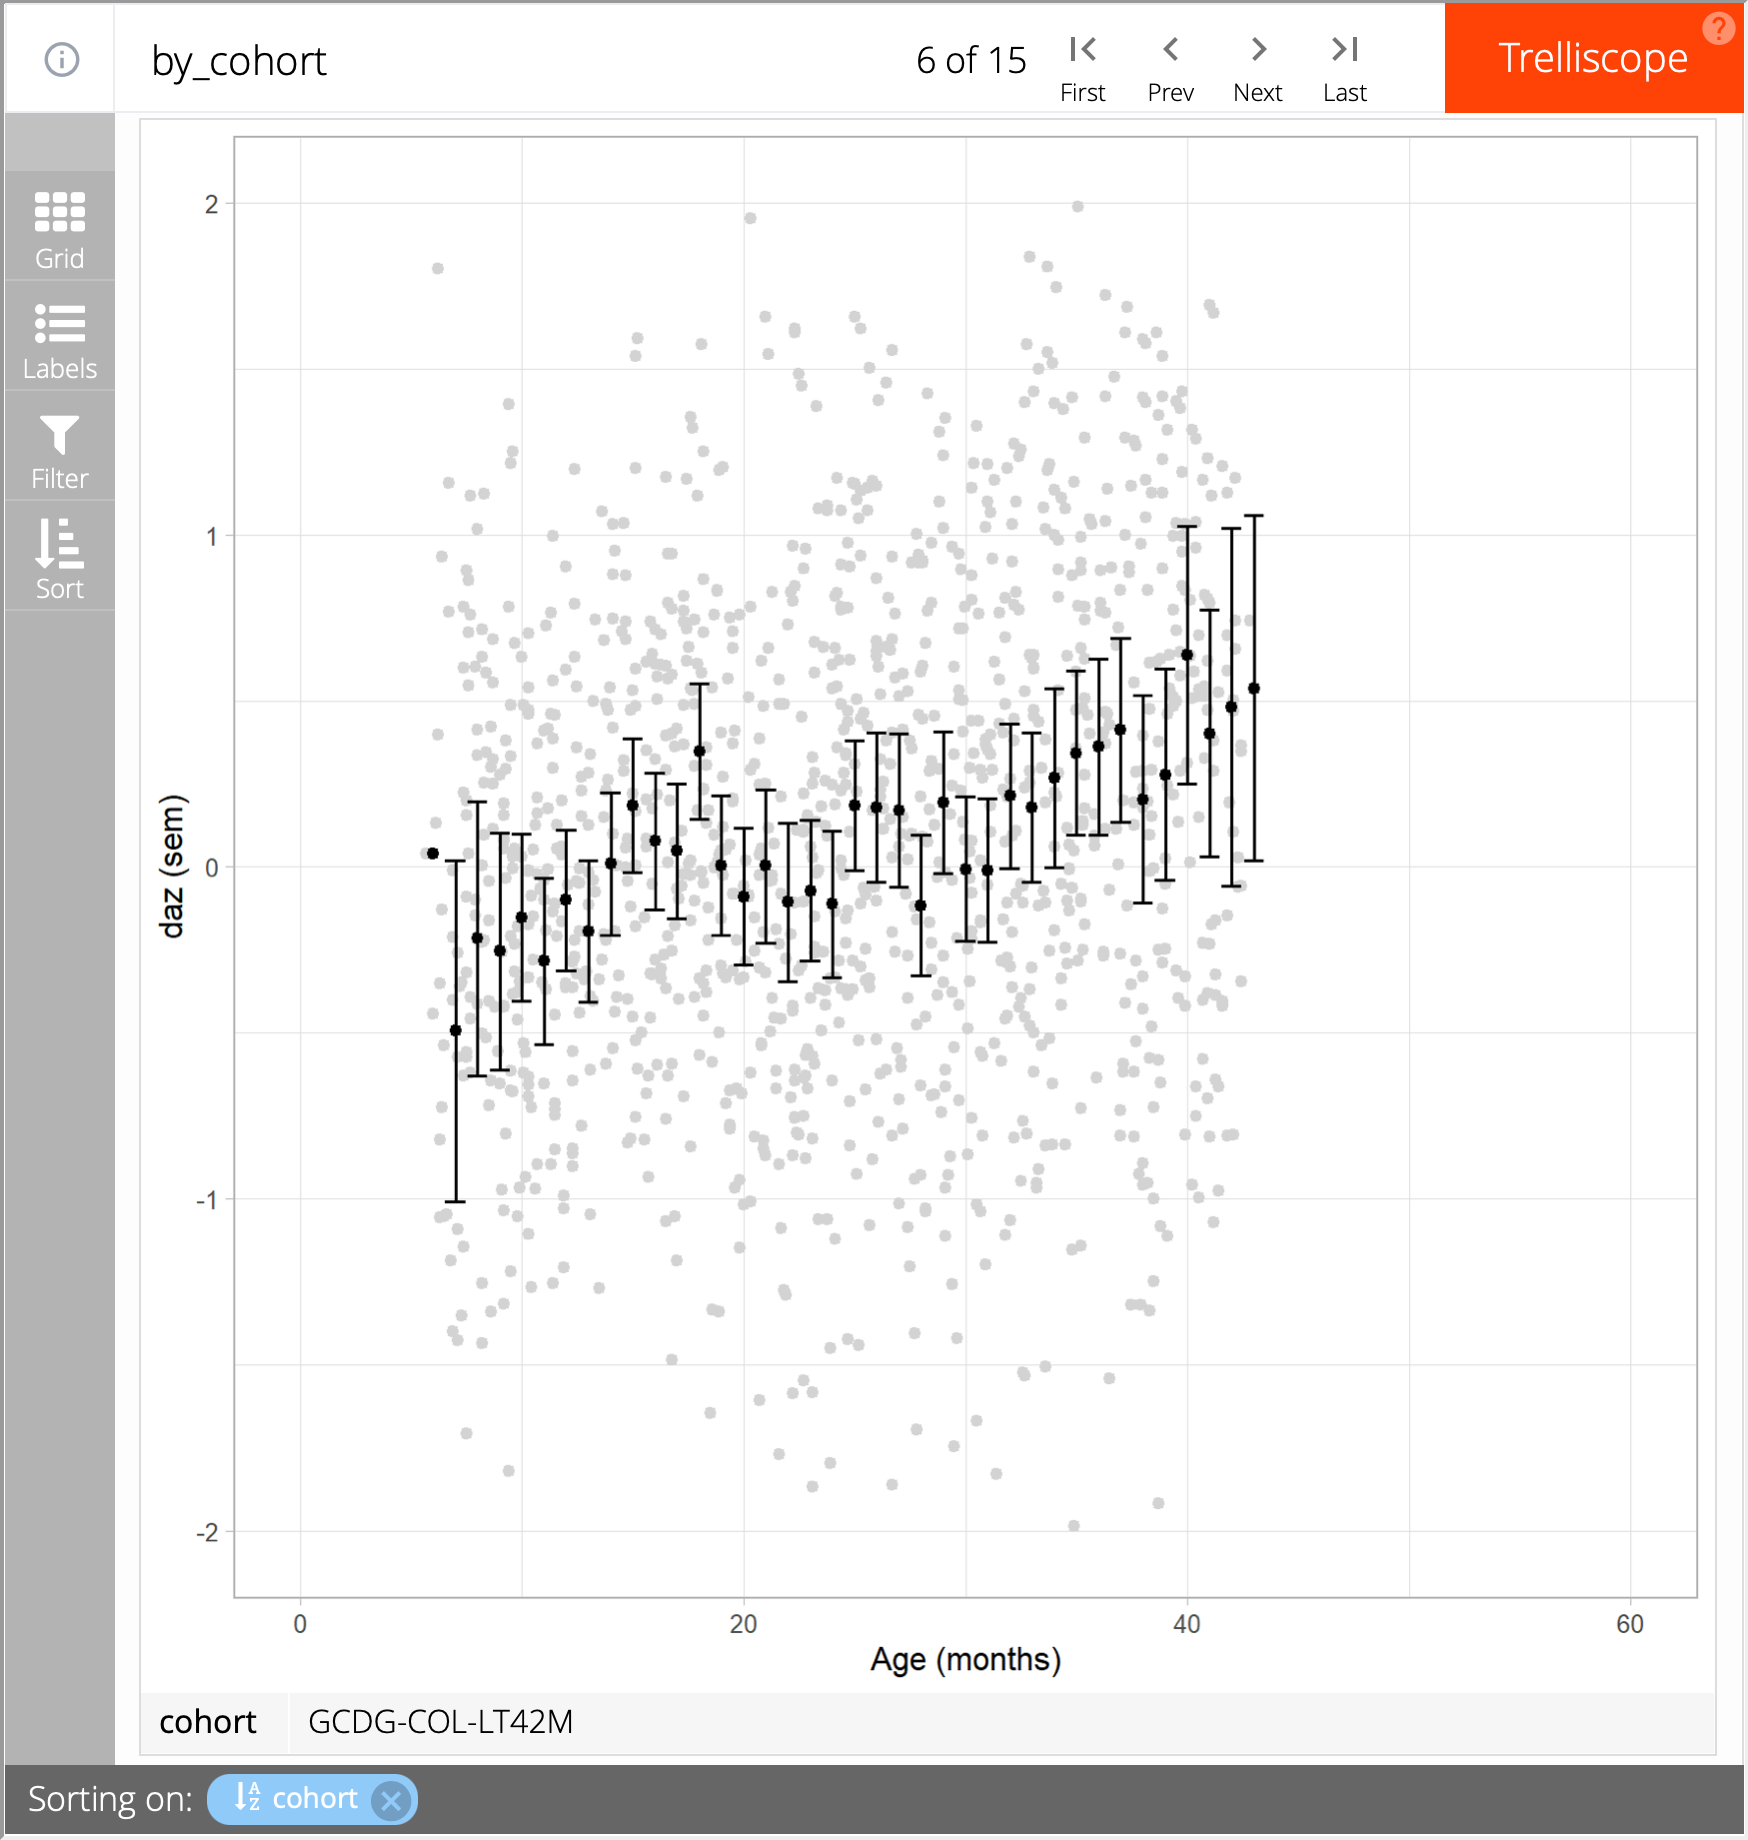
\includegraphics[width=1\linewidth]{fig/fig_6.4} 

}

\caption{\href{https://d-score.org/dbook-apps/gcdgsem/\#display=by_cohort\&nrow=1\&ncol=1\&arr=row\&pg=6\&labels=cohort\&sort=cohort;asc\&filter=\&sidebar=\&fv=}{The standard error of measurement (\(sem\)) around the age-standardized D-scores (DAZ) per cohort} (\url{https://d-score.org/dbook-apps/gcdgsem}).}\label{fig:dscoresems}
\end{figure}



Does precision vary with studies? The answer is yes. Figure \ref{fig:dscoresems} plots the same information as before but now broken down according to cohort. Individual data points are added to give a feel for the design. The Colombia cohort \texttt{GCDG-COL-LT45M} administered the Bayley-III, where each child answered on average 45 items, so the \emph{sem} is small. In contrast, the Dutch cohort GCDG-NLD-SMOCC collected data on a screener consisting of about ten relatively easy milestones, so the \emph{sem} is relatively large. As a result, the Colombian D-scores are much more precise than the Dutch.

\begin{figure}

{\centering 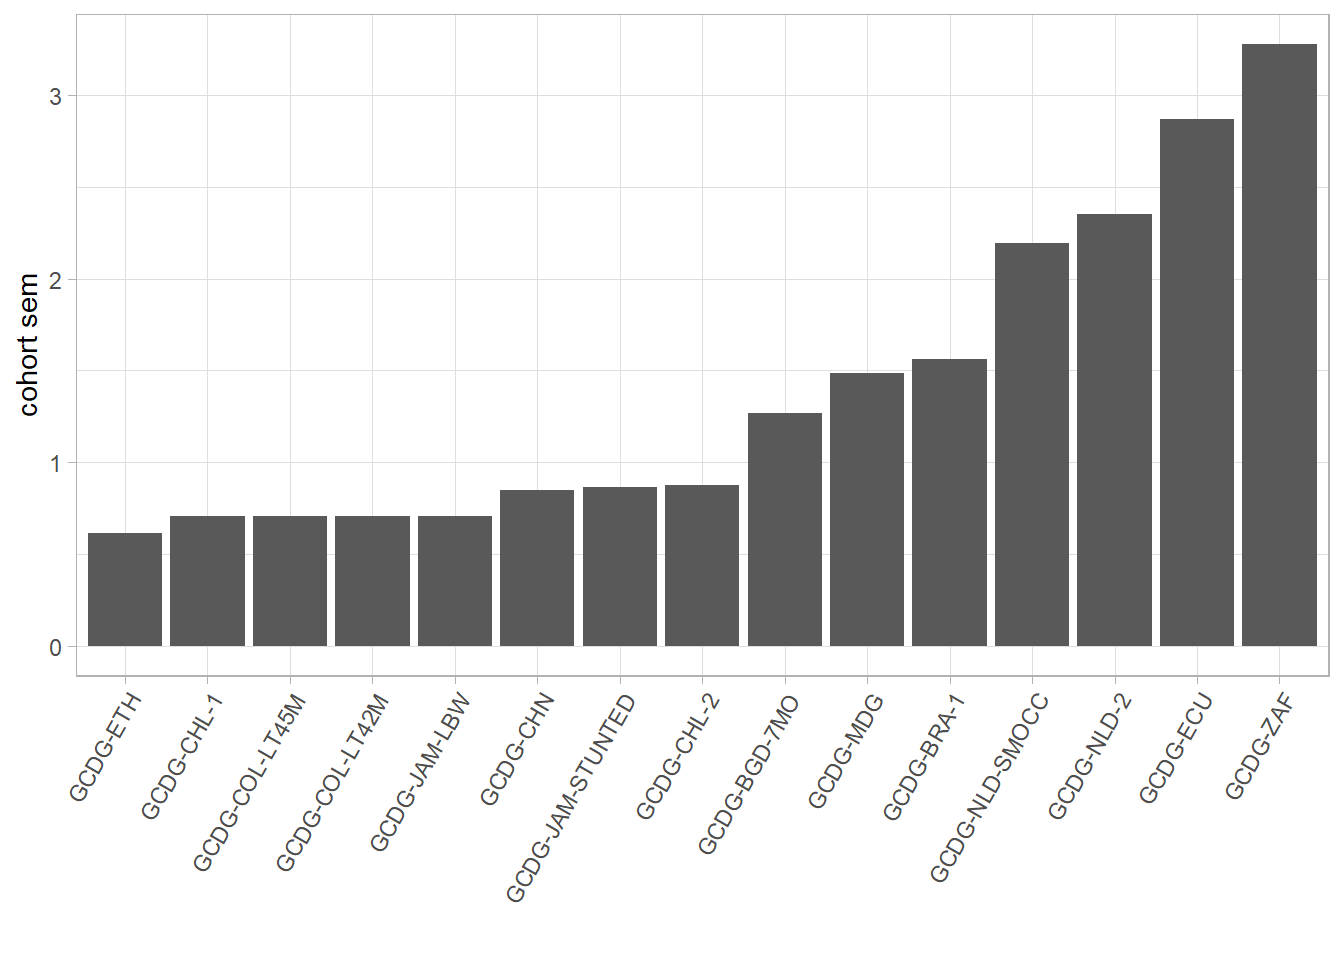
\includegraphics[width=1\linewidth]{dbook2_files/figure-latex/cohortsem-1} 

}

\caption{Cohort Standard Error of Measurement (\emph{sem}).}\label{fig:cohortsem}
\end{figure}



Figure \ref{fig:cohortsem} summarises the \(sem\) over the members of each cohort. The Ethiopia study GCDG-ETH is the most precise. In contrast, the D-score values in studies from South Africa, Ecuador and The Netherlands have sizeable measurement error.

\begin{table}

\caption{\label{tab:npsem}Test length and probability to pass the items per cohort}
\centering
\begin{tabular}[t]{lrr}
\toprule
Cohort & Test length & Pass probability\\
\midrule
GCDG-ETH & 39 & 0.66\\
GCDG-CHL-1 & 32 & 0.67\\
GCDG-COL-LT45M & 45 & 0.64\\
GCDG-COL-LT42M & 61 & 0.62\\
GCDG-JAM-LBW & 43 & 0.55\\
\addlinespace
GCDG-CHN & 27 & 0.50\\
GCDG-JAM-STUNTED & 38 & 0.65\\
GCDG-CHL-2 & 33 & 0.48\\
GCDG-BGD-7MO & 14 & 0.38\\
GCDG-MDG & 8 & 0.35\\
\addlinespace
GCDG-BRA-1 & 18 & 0.89\\
GCDG-NLD-SMOCC & 10 & 0.80\\
GCDG-NLD-2 & 11 & 1.00\\
GCDG-ECU & 3 & 0.67\\
GCDG-ZAF & 12 & 1.00\\
\bottomrule
\end{tabular}
\end{table}

~

The ordering of studies depends on test length and item information. Table \ref{tab:npsem} shows the median number of items per child (test length) and the probability to pass the item. The Ethiopian cohort \texttt{GCDG-ETH} administered 39 milestones with a median probability of 0.66. In contrast, the South Africa study \texttt{GCDG-ZAF} measures 12 items which were all very easy for the sample at hand (median probability of 1.0). One may thus well explain the extremes by test length and item information.

In general, the design of the study has a significant impact on the precision of the measurement. \href{https://stefvanbuuren.name/dbook3/}{Booklet III} addresses the question how one may construct a measurement instrument that will be optimally precise given the goals of the research.

\hypertarget{sec:domains}{%
\section{Domain coverage}\label{sec:domains}}

The D-score is a one-number summary of early child development. Traditional instruments distinguish domains (like motor, communication, language and cognitive development) and some provide ways to calculate a total score. The D-score, on the other hand, is based on the notion that child development is a unidimensional latent construct and hence does not provide domain scores. And thus, the question is how the D-score represents domains.

This section explores the following two questions:

\begin{itemize}
\tightlist
\item
  Can we break down the D-score by domain contribution, and if so, can we evaluate whether the D-score fairly represents all domains?
\item
  Can we calculate domain-specific D-scores?
\end{itemize}

\hypertarget{domain-coverage-of-the-scale}{%
\subsection{Domain coverage of the scale}\label{domain-coverage-of-the-scale}}

For many items in the D-score model, we had expert information available as to which domain the item belongs. For each item, we calculated the proportion of times the experts assigned it to one of five domains: Fine Motor, Gross Motor, Expressive, Receptive, Cognitive. We then calculated the distribution of domain by age.

\begin{figure}

{\centering 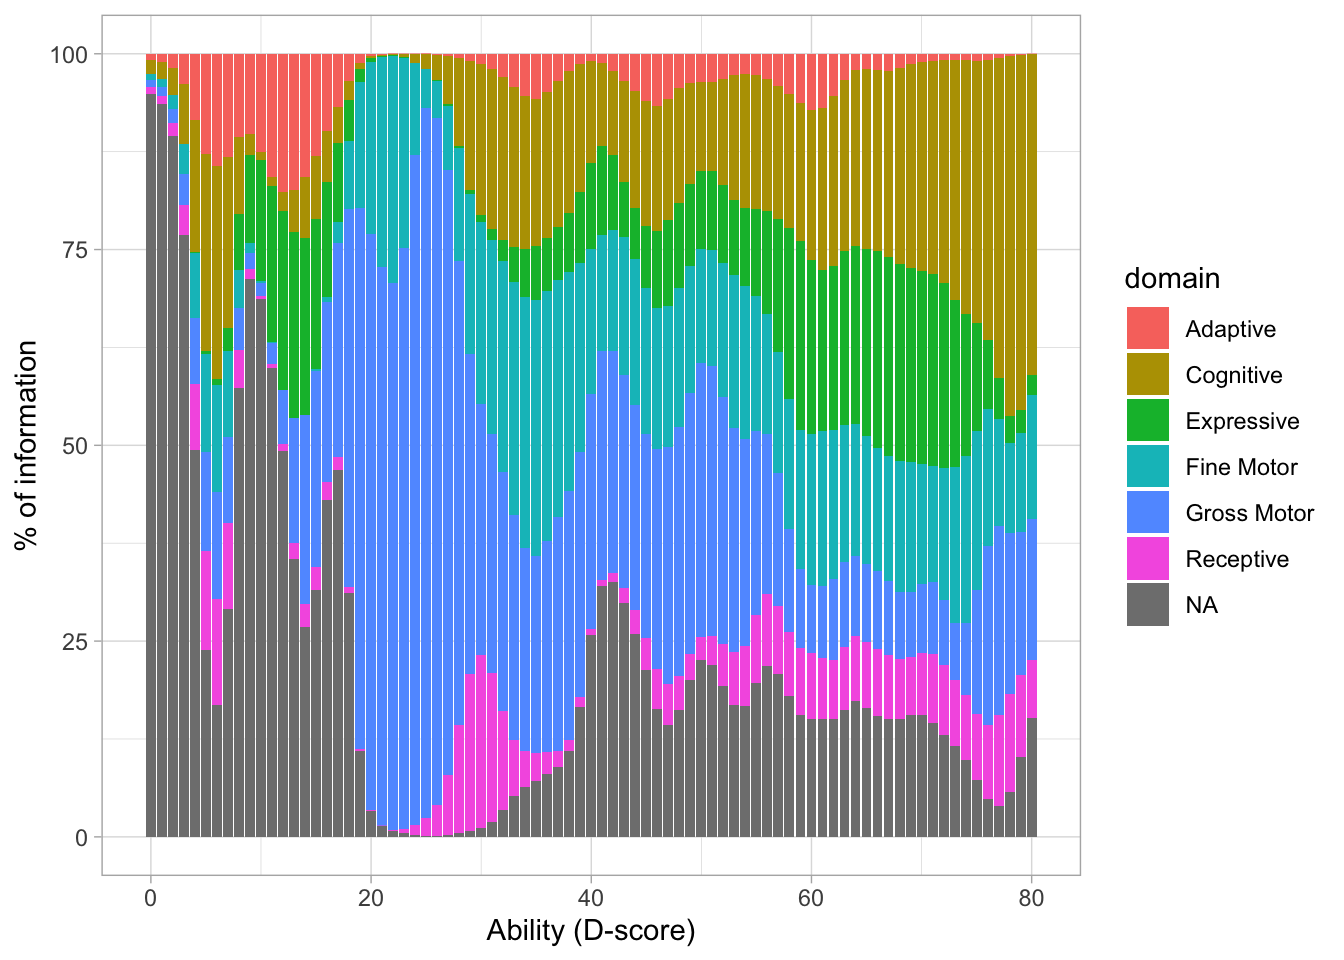
\includegraphics[width=1\linewidth]{dbook2_files/figure-latex/domaincov-1} 

}

\caption{Domain coverage of the D-score scale.}\label{fig:domaincov}
\end{figure}



Figure \ref{fig:domaincov} shows the domain composition of the D-score across different levels of ability. Note that we miss domain information for a few items. The share of gross-motor is large in early development (e.g., between 15 and 30 months), and gradually tapers off at higher levels. Reversely, the percentage of cognition and language is relatively small before 30 months but rapidly rises as the child matures. These transitions in domain composition look both reasonable and valid.

\hypertarget{domain-specific-d-scores}{%
\subsection{Domain-specific D-scores}\label{domain-specific-d-scores}}

Suppose we select a domain of interest and calculate the D-score only from items that substantially load onto that domain. We then get a domain-specific D-score. Items that relate to multiple domains contribute to multiple domain-specific D-scores.

\begin{figure}

{\centering 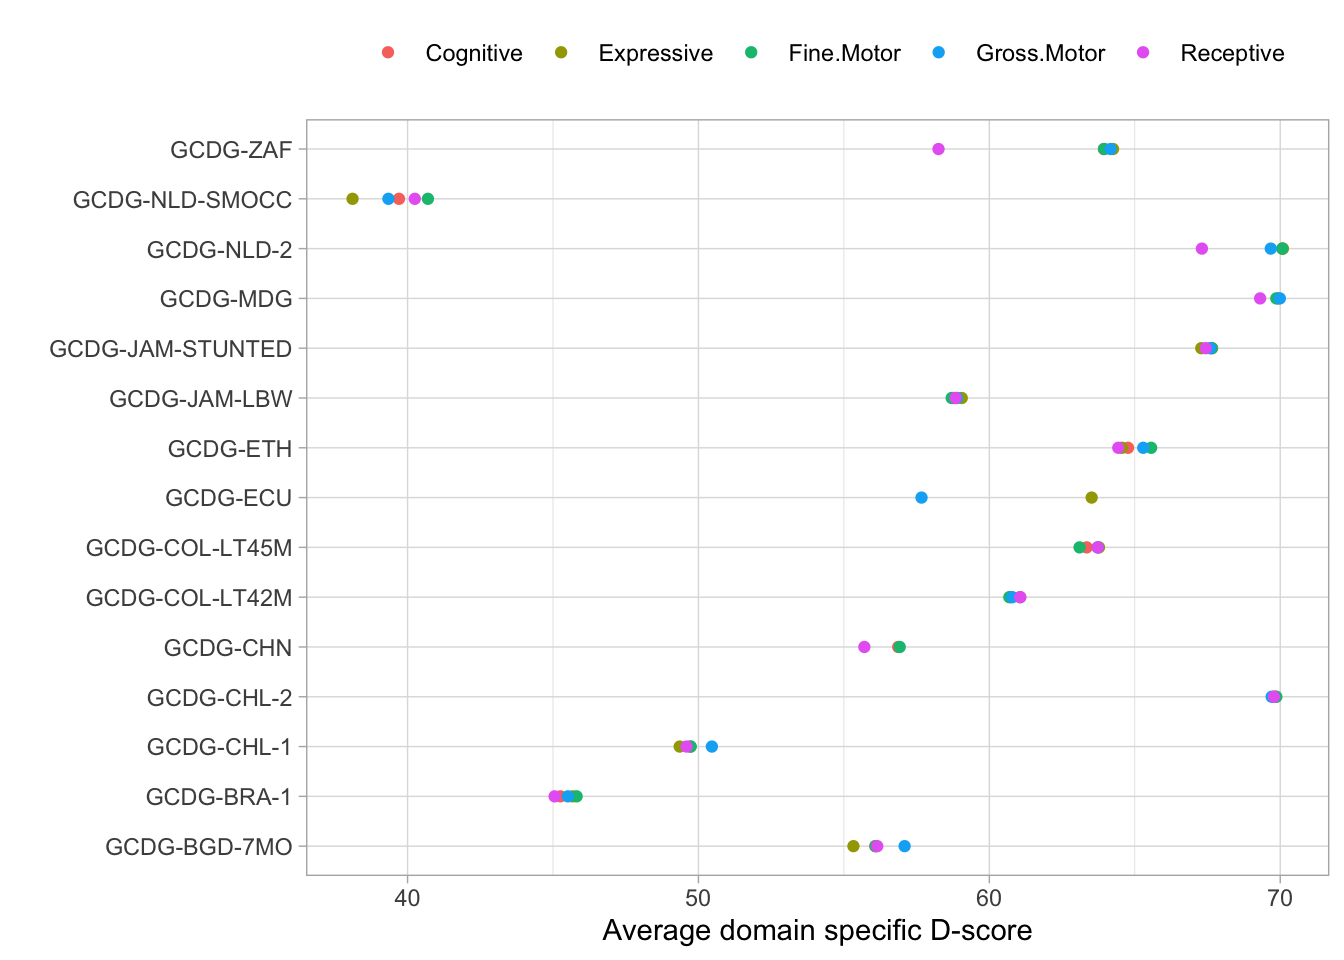
\includegraphics[width=1\linewidth]{dbook2_files/figure-latex/domaind-1} 

}

\caption{Average domain-specific DAZ \(\pm\) \emph{sem} by cohort.}\label{fig:domaind}
\end{figure}



Figure \ref{fig:domaind} displays the standardized domain-specific D-score (i.e.~DAZ) per cohort. The DAZ strips out irrelevant age variation, and thus enhances comparability between cohorts. The error bars around the scores depict the \emph{sem} interval. We observe some variation in domain-specific DAZ scores within cohorts. Still, these differences are relatively small and well within the margins of error. This analysis suggests that the D-score is an excellent overall summary of the domain-specific D-scores.

The D-score methodology assumes that child development is a unidimensional scale. As a consequence, the correlations between different domain-specific D-scores are extremely high (\(r > 0.95\)). It is more interesting to study the correlation between the DAZ equivalent of the domain-specific scores.

\begin{table}

\caption{\label{tab:domaincor}Pearson correlation of the DAZ and five domain-specific DAZ scores}
\centering
\begin{tabular}[t]{l|r|r|r|r|r|r}
\hline
  & DAZ & Fine motor & Gross Motor & Cognitive & Receptive & Expressive\\
\hline
DAZ & 1.00 & 0.69 & 0.57 & 0.84 & 0.70 & 0.69\\
\hline
Fine motor & 0.69 & 1.00 & 0.40 & 0.74 & 0.50 & 0.39\\
\hline
Gross Motor & 0.57 & 0.40 & 1.00 & 0.43 & 0.34 & 0.30\\
\hline
Cognitive & 0.84 & 0.74 & 0.43 & 1.00 & 0.76 & 0.59\\
\hline
Receptive & 0.70 & 0.50 & 0.34 & 0.76 & 1.00 & 0.63\\
\hline
Expressive & 0.69 & 0.39 & 0.30 & 0.59 & 0.63 & 1.00\\
\hline
\end{tabular}
\end{table}

~

Table \ref{tab:domaincor} lists the Pearson correlation matrix of the DAZ and the five domain-specific DAZ scores. All correlations between the DAZ and the domain-specific scores are high, thus confirming the generic character of the D-score and DAZ. We find high inter-domain correlations for the cognitive-receptive, cognitive-fine motor and expressive-receptive pairs. The gross motor domain appears as somewhat distinct from the four other domains. Its position may be genuine, but could also be related to the smaller number of responses on gross motor milestones in the GCDG data.

\begin{figure}

{\centering 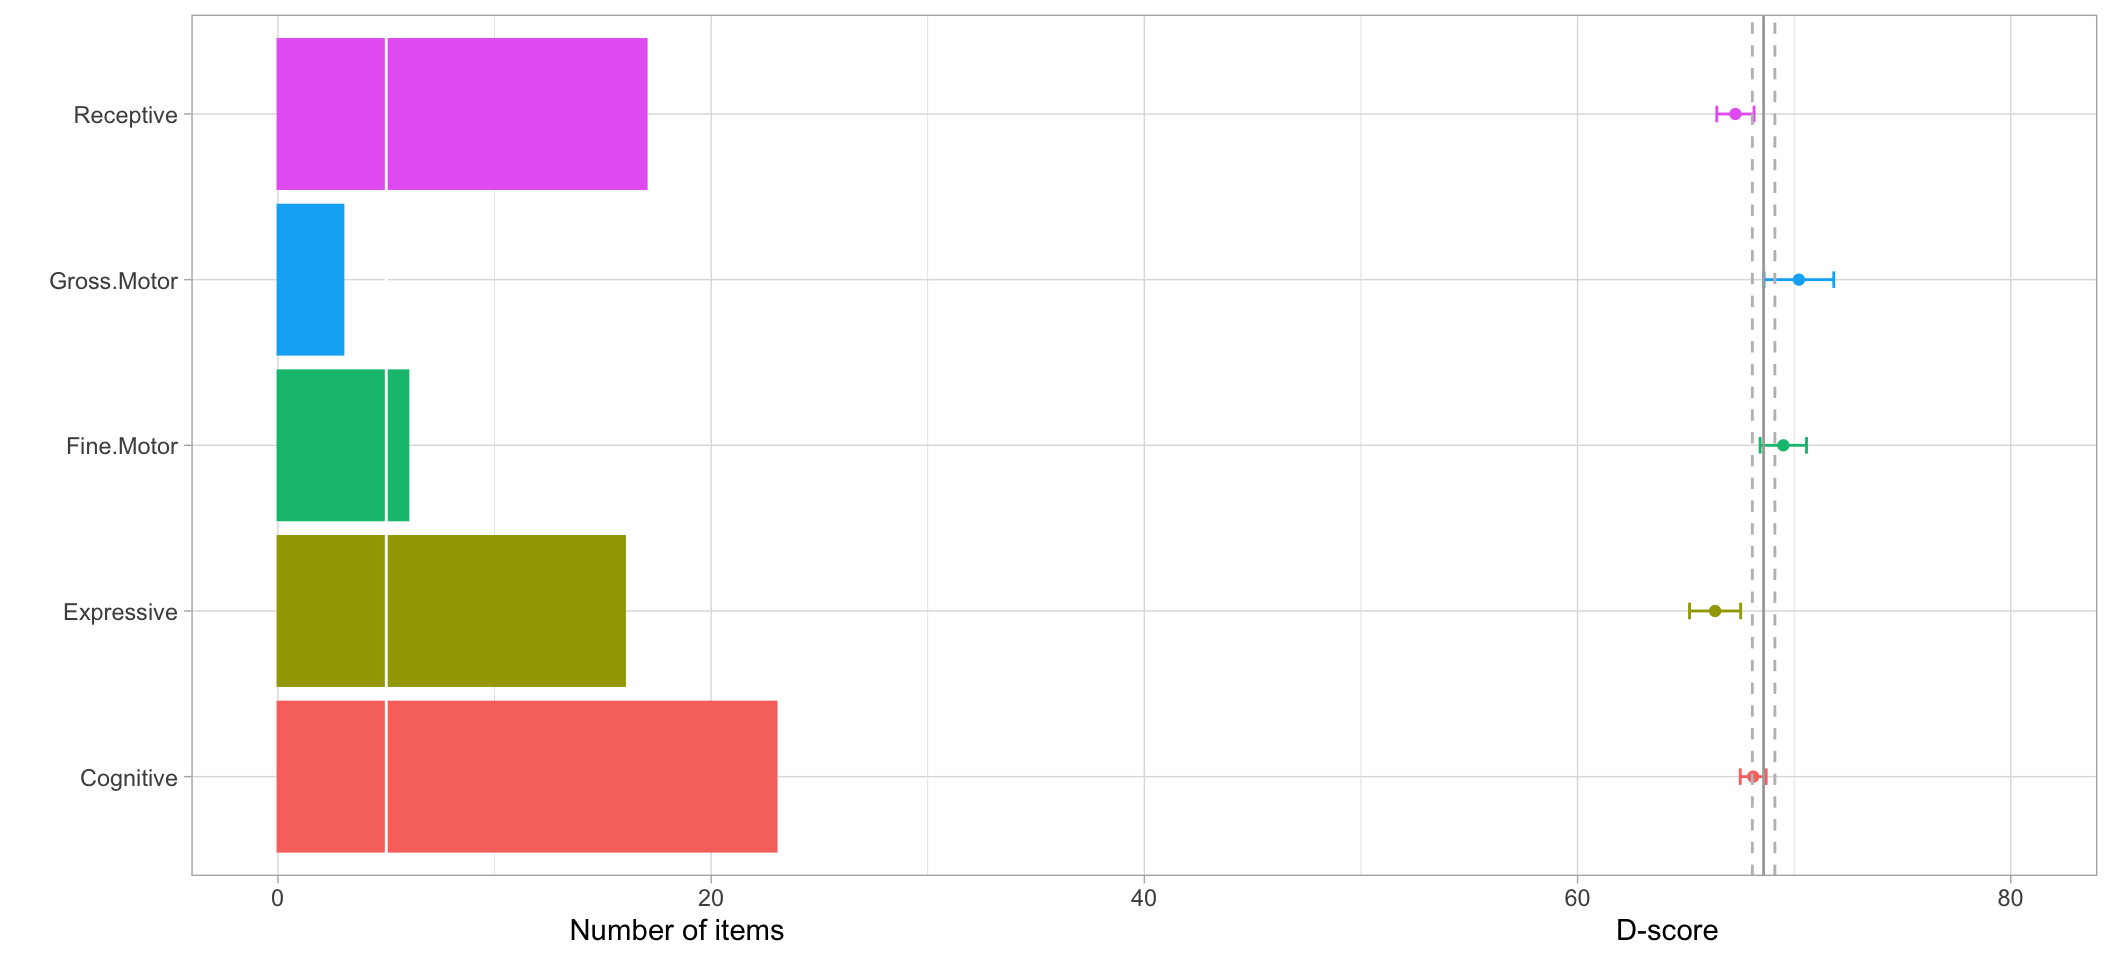
\includegraphics[width=1\linewidth]{dbook2_files/figure-latex/domaindex-1} 

}

\caption{Domain-specific D-scores for a 3 year old boy.}\label{fig:domaindex}
\end{figure}



Figure \ref{fig:domaindex} displays individual scores for a 3 year old boy. The filled bars indicate the number of available items per domain. The vertical white line that crosses the horizontal axis at value 5 indicates a threshold for a minimum number of items needed for a D-score. Note that the number of items for Gross Motor in this example is meagre (only three items). The grey vertical line indicates the value of the overall D-score (68.55\(D\)). The nearby dashed lines are located at one \emph{sem} (0.53\(D\)) distance. The coloured points are the domain-specific D-scores with the \emph{sem} around in error bars. The plot visualises that the boys' scores on language domains (i.e.~Expressive and Receptive) are low as compared to the motor and cognitive domains. A systematic discrepancy between various domain-specific scores might be an early warning sign for developmental delay.

\hypertarget{ch:SDGindicator}{%
\chapter{Application I: Tracking a Sustainable Development Goal}\label{ch:SDGindicator}}

\begin{quote}
Author: Iris Eekhout
\end{quote}

The Sustainable Development Goals (SDG) formulated by the United Nations (UN) set targets to promote prosperity while protecting the planet. One or more indicators quantify the progress towards each target.

This chapter explores the use of the D-score to monitor the progress of the indicator for healthy child development, SDG 4.2.1. We propose a method to define on-track development and show how the application of this method pans out for the GCDG data. More in detail, the chapter deals with the following topics:

\begin{itemize}
\tightlist
\item
  Estimating SDG 4.2.1 indicator from existing data (\ref{sec:application1})
\item
  Defining \emph{developmentally on track} (\ref{sec:references})
\item
  Country-level estimations (\ref{sec:countrytrack})
\item
  Relation to other estimates (\ref{sec:otherestimates})
\end{itemize}

\hypertarget{sec:application1}{%
\section{Estimating SDG 4.2.1 indicator from existing data}\label{sec:application1}}

The \href{https://www.un.org/sustainabledevelopment/development-agenda/}{UN Sustainable Development Goals} form a universal call to action to end poverty, protect the planet and improve the lives and prospects of everyone, everywhere. All UN Member States adopted the 17 Goals in 2015. The SDG 4 target to ensure inclusive and equitable quality education and promote lifelong learning opportunities for all. SDG 4.2 reads as:

\begin{quote}
By 2030, ensure that all girls and boys have access to quality early childhood development, care and preprimary education so that they are ready for primary education.
\end{quote}

To measure progress, the UN defined indicator 4.2.1 as follows:

\begin{quote}
Proportion of children under 5 years of age who are developmentally on track in health, learning and psychosocial well-being, by sex.
\end{quote}

On July 22, 2020, the indicator was \href{https://unstats.un.org/sdgs/metadata/}{changed} into

\begin{quote}
Proportion of children aged 24-59 months who are developmentally on track in health, learning and psychosocial well-being, by sex.
\end{quote}

The exclusion of children 0-24 months is at variance with the importance of healthy growth and development during the first 1000 days of life. Indeed, the UN restricted the age range for practical concerns. \protect\hyperlink{ref-loizillon2017}{Loizillon et al.} (\protect\hyperlink{ref-loizillon2017}{2017}) report:

\begin{quote}
The initial recommendation was for the ECDI to measure child development from birth--5 years, but the range was restricted to 3--5 years due to time and resource constraints and limited availability of comparable measurement tools for children under age 3.
\end{quote}

The careful scientific approach underlying the D-score fills the gap for children aged 0-24 months. Also, the D-score methodology enables extensions to ages beyond 24 months, permits back-calculation of D-scores from existing data, and acts as a linking pin to compare child development from birth onwards.

The cohorts included in the GCDG study represent a wide range of countries and instruments (see Section \ref{sec:gcdgoverview}). Combining existing data from such a wide range of countries to create the D-score, is undoubtedly challenging, but doable. Although, in all fairness, we note that obtaining accurate comparisons between world-wide populations requires additional representative (existing) data beyond what is available here.

\hypertarget{sec:references}{%
\section{\texorpdfstring{Defining \emph{developmentally on track}}{Defining developmentally on track}}\label{sec:references}}

In 2006, the World Health Organisation (WHO) published the \href{https://www.who.int/childgrowth/publications/technical_report_pub/en/}{WHO Child Growth Standards}. These standards specify ``how children should grow'' and form the basis for widely used anthropometric indicators such as stunting and wasting. We advocate a similar approach for child development. More in particular, the following steps:

\begin{enumerate}
\def\labelenumi{\arabic{enumi}.}
\tightlist
\item
  Measure child development on an interval scale;
\item
  Estimate the age-conditional reference distribution for normal child development;
\item
  Define the indicator \emph{developmentally on track} as the proportion above a chosen cut-off.
\end{enumerate}

Step 1 is solved by the D-score. Step 2 borrows from well-tested statistical methodology for constructing growth standards (\protect\hyperlink{ref-borghi2006}{Borghi et al. 2006}). Step 3 can be done in different ways, but a applying a simple cut-off fits easily with regular practice in reporting international comparisons.

\begin{figure}

{\centering 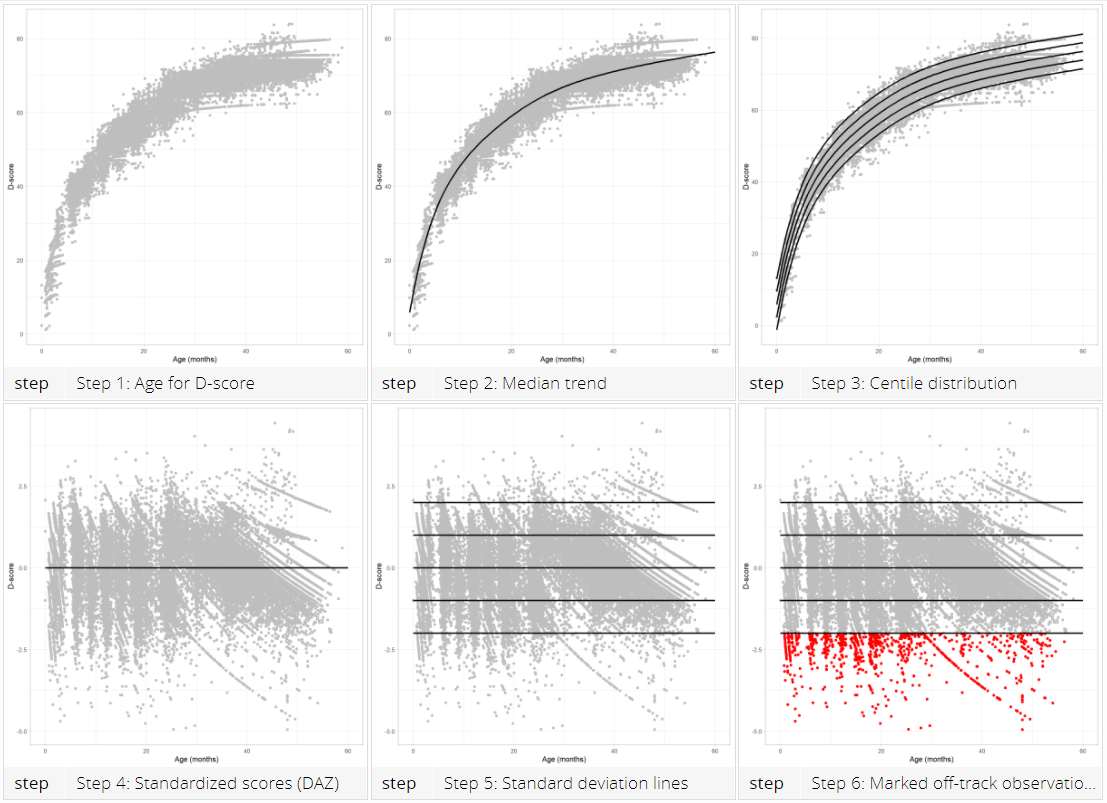
\includegraphics[width=1\linewidth]{fig/fig_7.1_full} 

}

\caption{\href{https://d-score.org/dbook-apps/gcdgreferences/}{Illustration of the method to define on-track development} (\url{https://d-score.org/dbook-apps/gcdgreferences/}).}\label{fig:dscorerefs}
\end{figure}



Figure \ref{fig:dscorerefs} demonstrates steps 2 and 3 in more detail. Click `Next' to advance a series of six steps:

\begin{enumerate}
\def\labelenumi{\arabic{enumi}.}
\tightlist
\item
  Plot the D-score by age;
\item
  Model the relation between age and D-score by an LMS model. In practice, this amounts to smoothing three curves representing the median, coefficient of variation and the skewness.
\item
  Present the centile lines for the model;
\item
  Plot the age-standardized scores for development (DAZ);
\item
  Draw standard deviation lines to indicate the location at \(\pm\) 1 and \(\pm\) 2 standard deviation from the mean;
\item
  Count observations above the -2 SD line as on-track. Count observation below the -2 SD lines as off-track (red dots).
\end{enumerate}

\emph{Note: These SD lines build upon on a convenience sample. The GCDG cohorts are not representative samples, and the countries are not representative of the world. While we should not over-interpret these references, they play a central role in a stepwise, principled approach to define ``developmentally on track.''}

\hypertarget{sec:countrytrack}{%
\section{Country-level estimations}\label{sec:countrytrack}}

\begin{table}

\caption{\label{tab:ontrack}Percentage of on-track children per country}
\centering
\begin{tabular}[t]{l|r}
\hline
Country & Percentage on-track\\
\hline
BGD & 94.9\\
\hline
BRA & 99.5\\
\hline
CHL & 98.3\\
\hline
CHN & 99.9\\
\hline
COL & 98.9\\
\hline
ECU & 93.9\\
\hline
ETH & 99.4\\
\hline
JAM & 99.6\\
\hline
MDG & 96.6\\
\hline
NLD & 96.8\\
\hline
ZAF & 97.4\\
\hline
\end{tabular}
\end{table}

~

Using the definition from the previous section, we can calculate the percentage of children that are developmentally on track. Table \ref{tab:ontrack} summarises this statistic by country. At a cut-off value of -2 SD, we expect that about 97.7\% of the children will be on track. The actual country estimates fall into the range 93.9 - 99.9 and are thus near the theoretical value. This close correspondence shows that the definition and estimation procedure work as expected.

Bear in mind that the measurements leading up to these estimates come from different instruments. It is gratifying to see how well we can do with historical data, thanks to the robust underlying measurement model. Of course, comparability only gets better if all countries would use the same instrument. However, using the same tool everywhere is not a requirement.

\hypertarget{sec:otherestimates}{%
\section{Off-track development and stunted growth}\label{sec:otherestimates}}

\protect\hyperlink{ref-Weber2019}{Weber et al.} (\protect\hyperlink{ref-Weber2019}{2019}) thoroughly discuss concurrent, discriminant and predictive validity of the D-score using the GCDG data. In this section, we concentrate on the relation between the D-score and stunting, a popular measure of impaired height growth in children due to nutrition problems. The WHO defines \href{https://www.who.int/nutrition/healthygrowthproj/en/index1.html}{stunted growth} as a height-for-age Z-score below the -2 SD line of the WHO Child Growth Standards (HAZ \textless{} -2.0).

\begin{figure}

{\centering 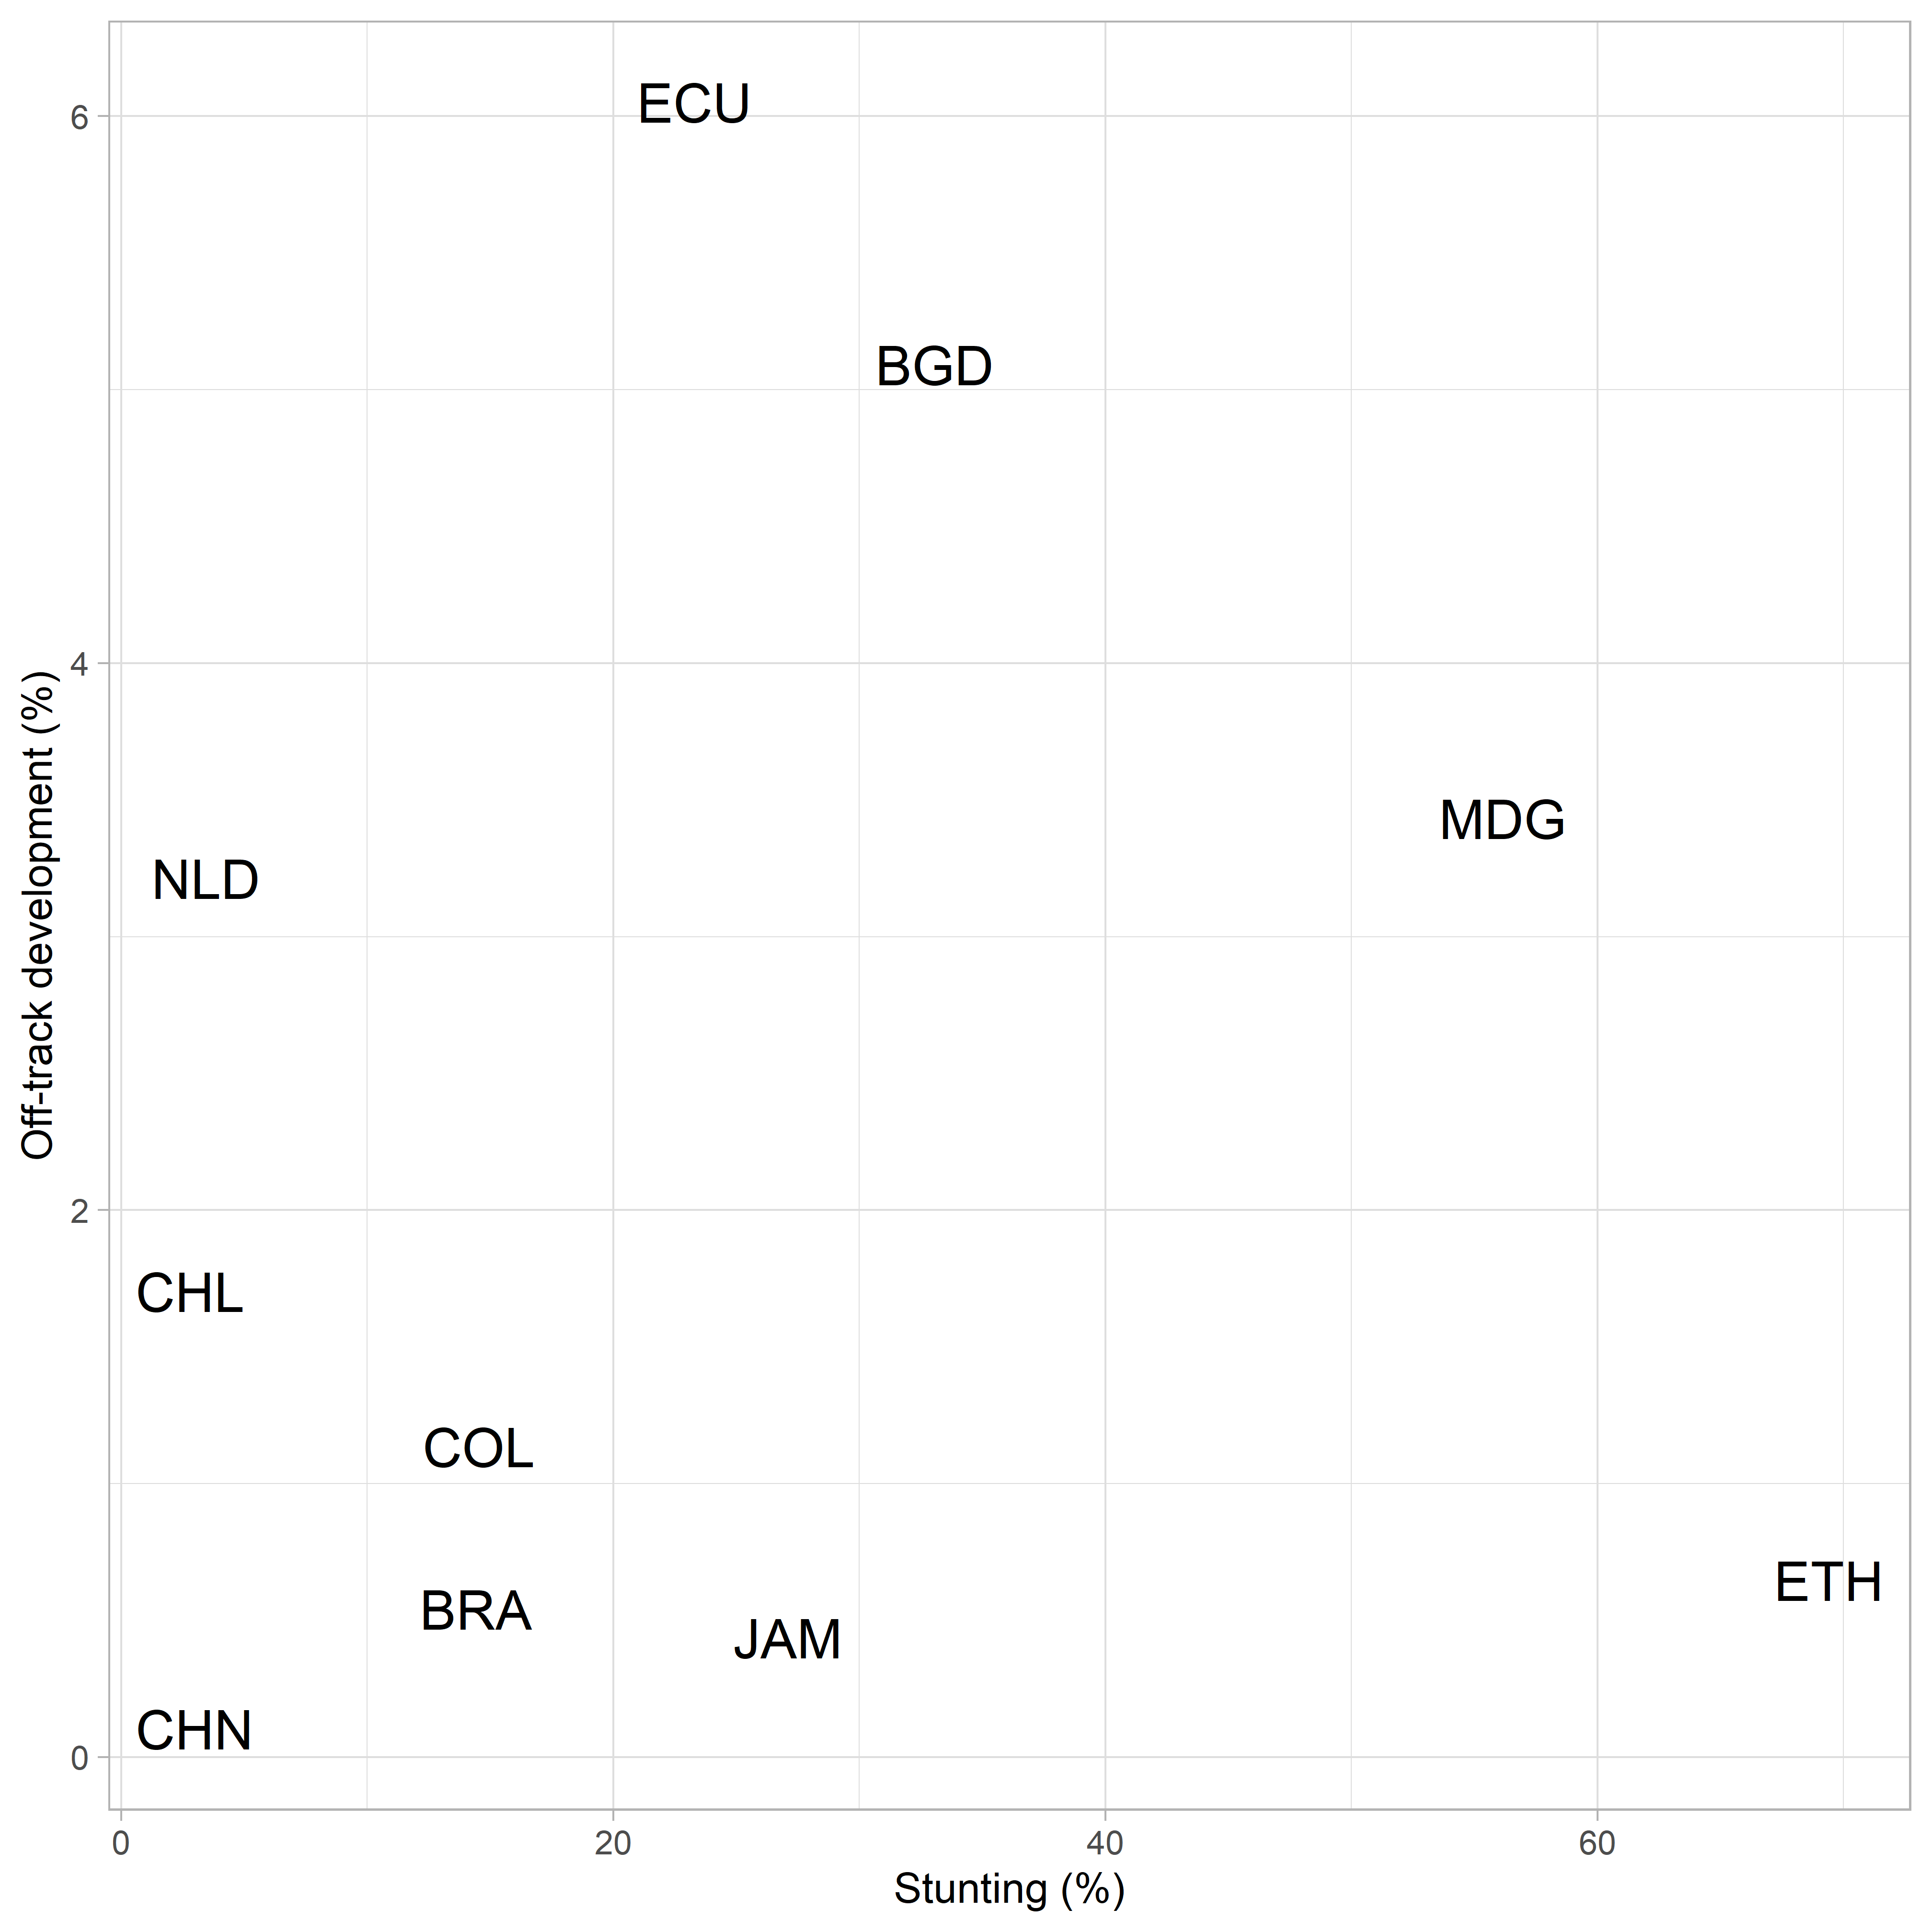
\includegraphics[width=1\linewidth]{dbook2_files/figure-latex/stunt-1} 

}

\caption{Off-track development (\%) versus stunting (\%) per country}\label{fig:stunt}
\end{figure}



Figure \ref{fig:stunt} plots the percentage off-track and percentage stunting per country. This plot reveals two exciting features:

\begin{itemize}
\tightlist
\item
  \emph{The variation in stunting is much larger than the variation off-track development}. One might speculate that height is more dependent on the environment than off-track development, and hence more variable.
\item
  \emph{Stunted growth and off-track development are unrelated}. Ranking countries by stunting or by off-track development yields substantially different orders. This finding provides clear counter-evidence to the argument that stunted growth is as a proxy for delayed development. It may even be the case the child development and physical growth are different maturation processes that develop largely independently.
\end{itemize}

\begin{figure}

{\centering 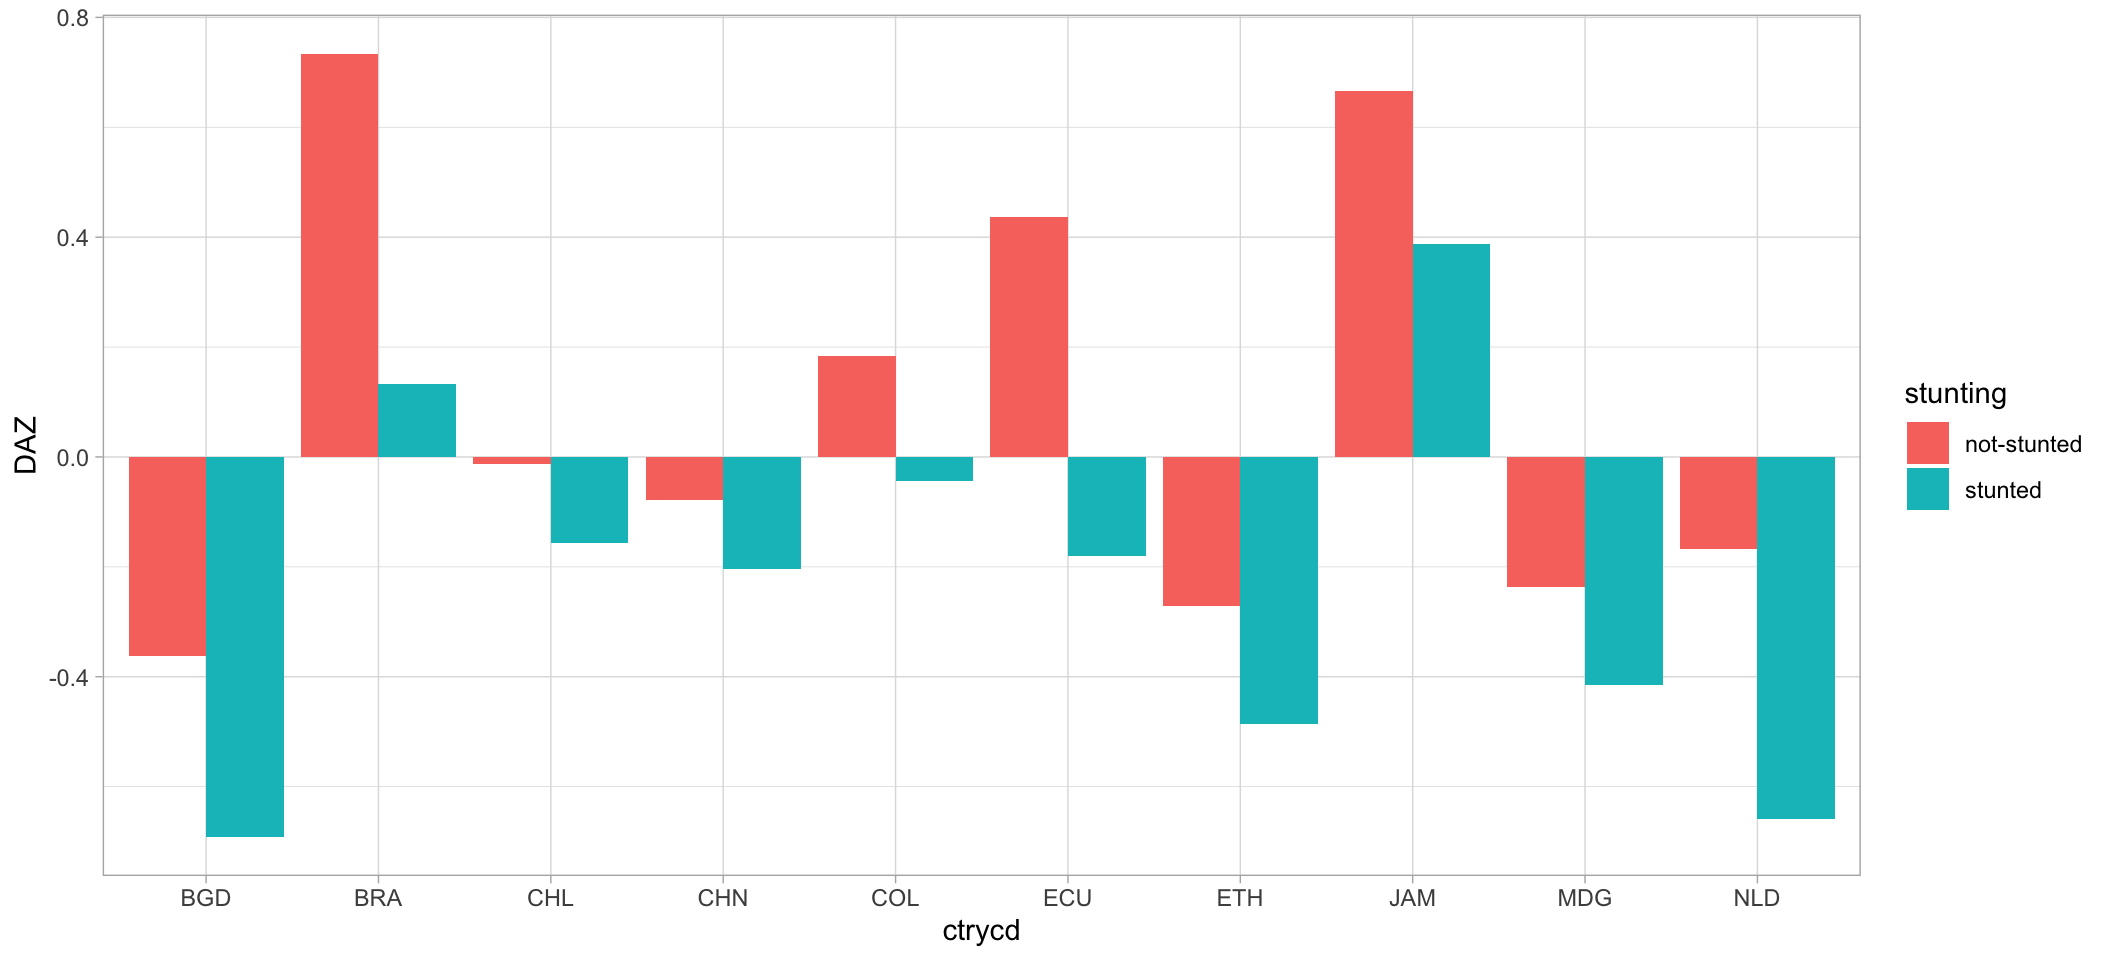
\includegraphics[width=1\linewidth]{dbook2_files/figure-latex/stuntdaz-1} 

}

\caption{Difference in mean DAZ per country between stunted and not stunted children.}\label{fig:stuntdaz}
\end{figure}



However, this is not the whole story. Figure \ref{fig:stuntdaz} reveals a consistent difference in DAZ between stunted and non-stunted children of about 0.2 - 0.3 SD. There could be factors at the child level that affect both development and height growth. For example, low-income families may lack the resources for adequate nutrition, which may impact both child development and physical growth.

The exact nature of the relation between stunting and development is still obscure. The D-score provides a means to study the intriguing interplay between both measures in more detail.

\hypertarget{ch:ontrack}{%
\chapter{Application II: Who is on-track?}\label{ch:ontrack}}

\begin{quote}
Author: Iris Eekhout
\end{quote}

Chapter \ref{ch:SDGindicator} described a method to define and estimate off-track development. The current chapter highlights strategies to find factors that discriminate between children that are on-track and off-track. We order explanatory factors relative to their importance and discuss opportunities for interventions.

\begin{itemize}
\tightlist
\item
  What determines who is developmentally on-track (\ref{sec:application2})
\item
  Factors that impact child development (\ref{sec:factors})
\end{itemize}

\hypertarget{sec:application2}{%
\section{What determines who is developmentally on-track?}\label{sec:application2}}

There are multiple ways to define on-track development. Here we will use the method outlined in section \ref{sec:references}. Ideally, we would like to fit the age-conditional reference distribution on a sample of children with normal, healthy development. As noted before, we calculated the references used in section \ref{sec:references} from a convenience sample. They may not be representative of healthy development.

\begin{figure}

{\centering 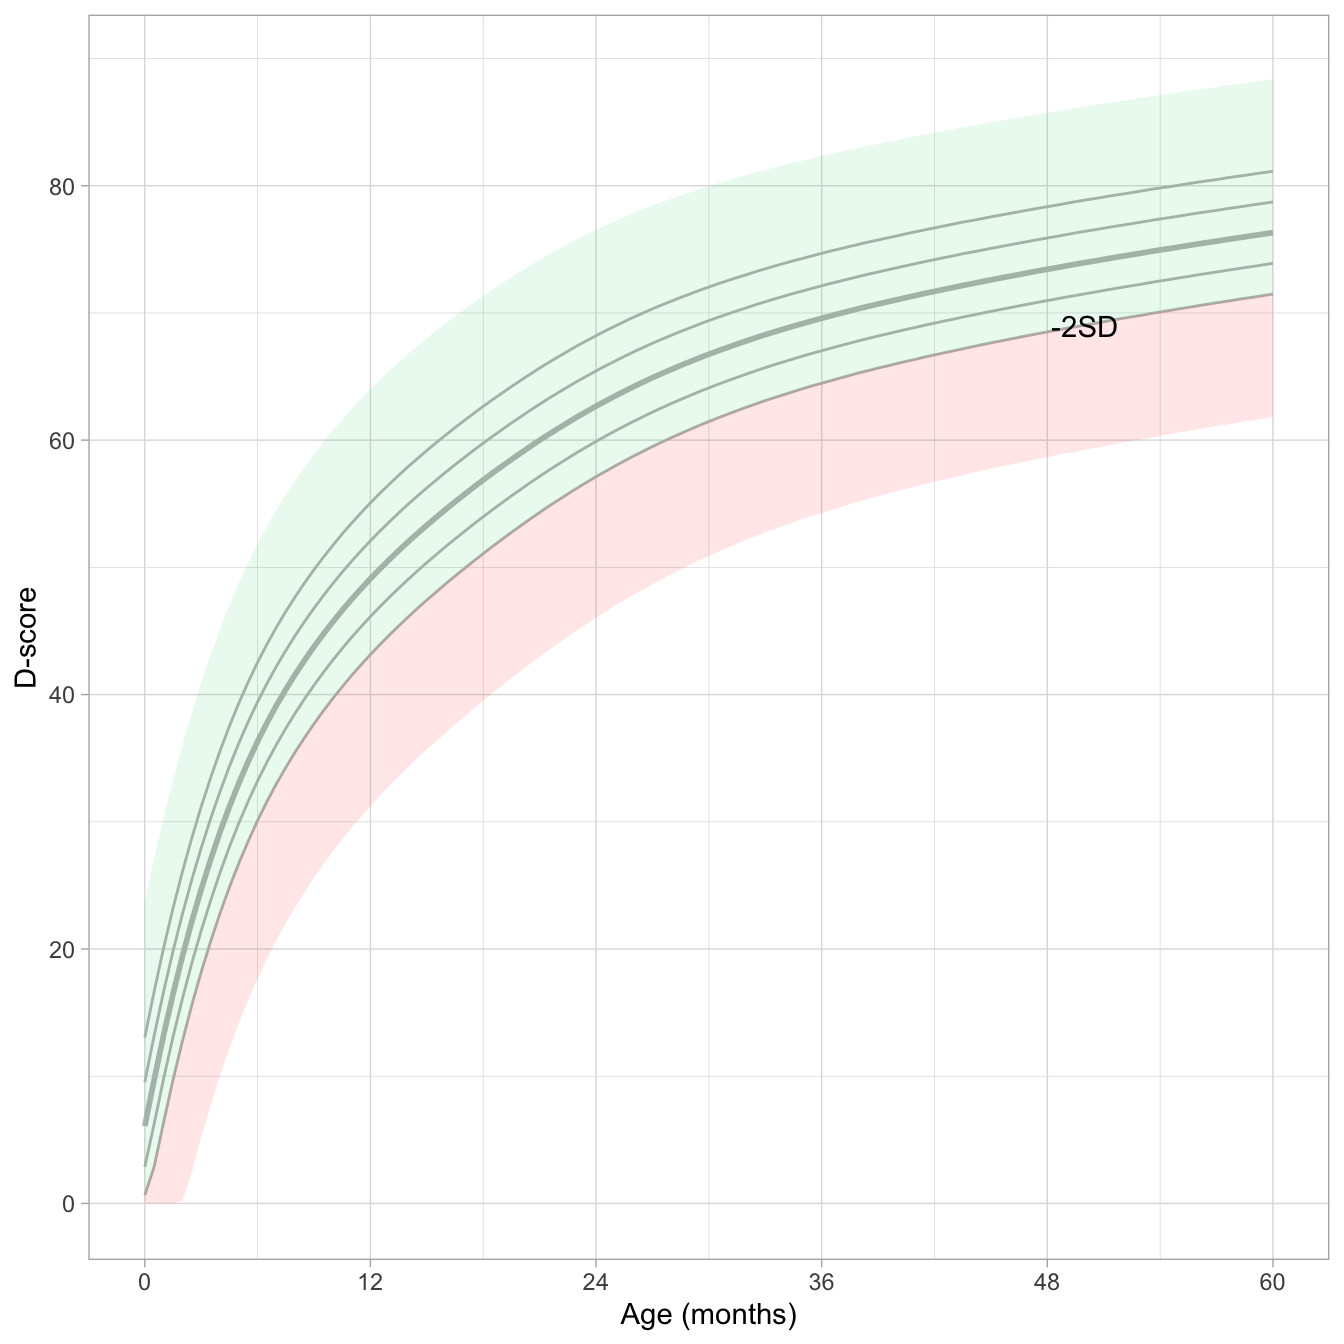
\includegraphics[width=1\linewidth]{dbook2_files/figure-latex/ontrackref-1} 

}

\caption{D-score observatations that are on-track according the current references.}\label{fig:ontrackref}
\end{figure}



Assuming we place the cut-off value at -2 SD, we may subdivide the observed D-scores into off-track and on-track. Figure \ref{fig:ontrackref} colours the regions of the D-score for children considered on-track (green) and off-track (red). The regions indicate the expected locations of D-scores in practice. Although one could find D-score outside the coloured areas, such should be very rare. The occurrence of such cases may indicate an error in the calculation of the D-score, most likely caused by setting an incorrect age variable.

Preventing observations in the red region requires us to form an idea about the factors that determine the off-track probability. The next section looks into this topic.

\hypertarget{sec:factors}{%
\section{Factors that impact child development}\label{sec:factors}}

We already know many of the factors that influence early child development. A higher level of education in the family promotes development. Infectious diseases like malaria slow down growth. Access to adequate nutrition, clean water and a stimulating, prosperous and safe environment is favourable for healthy development. And so on. Unfortunately, we do not have data on most factors, so we need to limit ourselves to a few background characteristics.

\begin{table}

\caption{\label{tab:ontracktab}Comparisons between on-track and off-track development}
\centering
\begin{tabular}[t]{l|l|r|r|r|r}
\hline
\multicolumn{2}{c|}{ } & \multicolumn{2}{c|}{On-track} & \multicolumn{2}{c}{Off-track} \\
\cline{3-4} \cline{5-6}
 &  & n & \% & n & \%\\
\hline
 & female & 21136 & 0.977 & 489 & 0.023\\
\cline{2-6}
\multirow[t]{-2}{*}{\raggedright\arraybackslash sex} & male & 20805 & 0.972 & 595 & 0.028\\
\cline{1-6}
 & <2500gr & 3388 & 0.948 & 185 & 0.052\\
\cline{2-6}
\multirow[t]{-2}{*}{\raggedright\arraybackslash birth weight} & >2500gr & 36375 & 0.978 & 821 & 0.022\\
\cline{1-6}
 & no education & 1907 & 0.967 & 66 & 0.033\\
\cline{2-6}
 & any primary & 11764 & 0.967 & 398 & 0.033\\
\cline{2-6}
 & any secondary & 21576 & 0.977 & 503 & 0.023\\
\cline{2-6}
\multirow[t]{-4}{*}{\raggedright\arraybackslash maternal education} & higher secondary & 6263 & 0.984 & 101 & 0.016\\
\cline{1-6}
 & rural & 1251 & 0.989 & 14 & 0.011\\
\cline{2-6}
 & semi-urban & 2236 & 0.990 & 23 & 0.010\\
\cline{2-6}
 & urban & 18740 & 0.971 & 566 & 0.029\\
\cline{2-6}
\multirow[t]{-4}{*}{\raggedright\arraybackslash residence} & metropolitan & 11122 & 0.979 & 234 & 0.021\\
\hline
\multicolumn{6}{l}{\textsuperscript{*} Exludes children with missing DAZ or missing factor}\\
\end{tabular}
\end{table}

~

Table \ref{tab:ontracktab} compares the frequency distributions of various factors for children on-track versus off-track. There are only tiny differences between boys and girls. Children with low birth weight (\textless{} 2500 gr) are more at risk for off-track development. This estimate does not correct for gestational age. We discussed techniques for such corrections \href{https://d-score.org/dbook1/sec-pops.html}{elsewhere}.

The influence of maternal education on off-track development follows the expected trend. Interestingly, it seems that a rural environment could prevent off-track development. We note that original measures of maternal education and residence were harmonised across studies. It would, therefore, also be interesting to study the impact per cohort using the actual factor coding.

\begin{figure}

{\centering 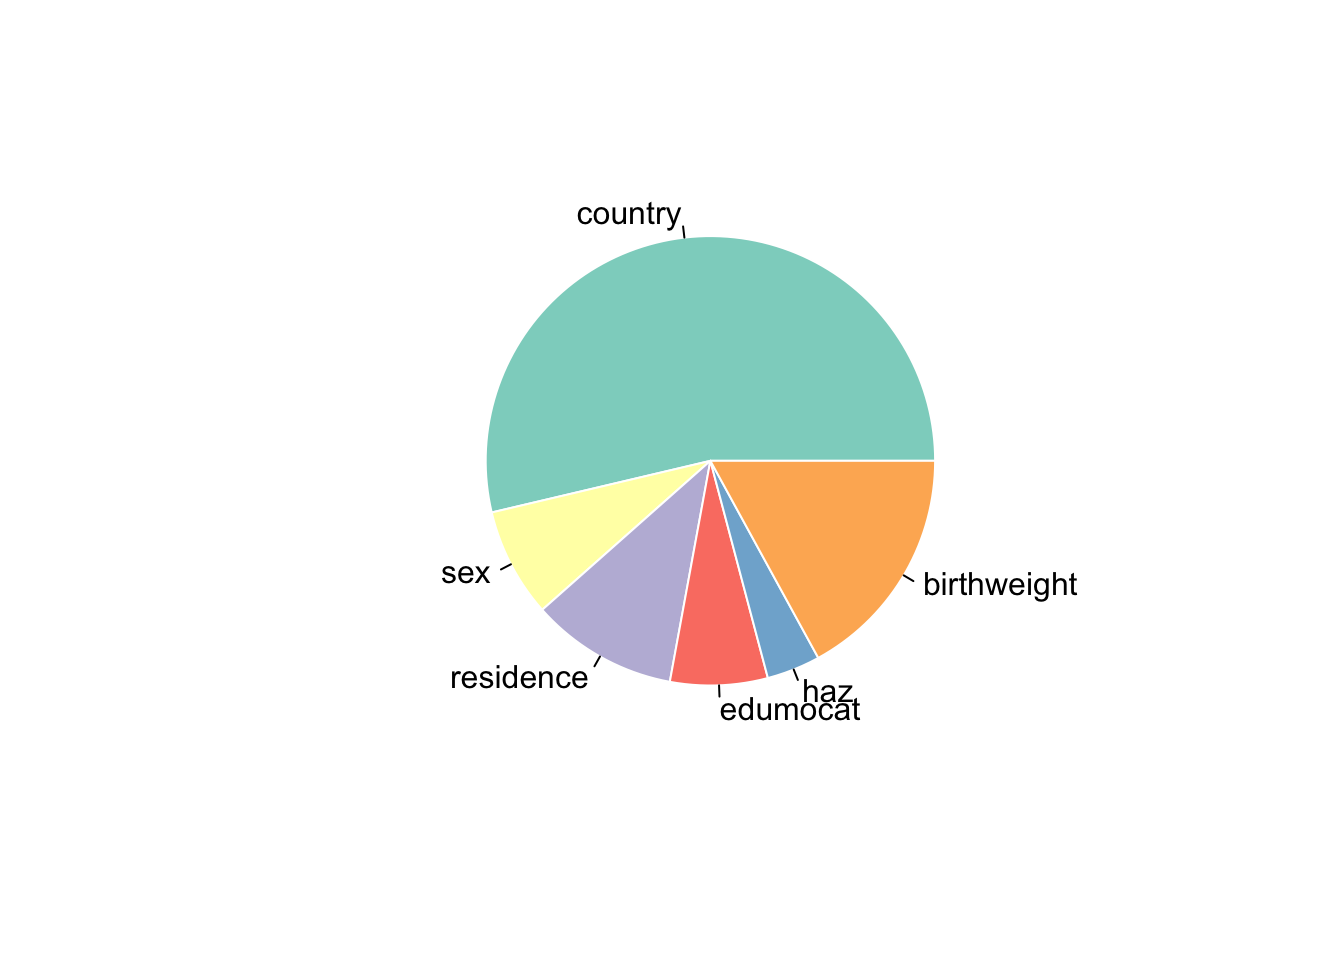
\includegraphics[width=1\linewidth]{dbook2_files/figure-latex/imppie-1} 

}

\caption{Relative importance of the explanatory factors in this study}\label{fig:imppie}
\end{figure}



We predicted DAZ by linear regressions with predictors country, sex, birth weight, maternal education, height for age and residential area. The percentage of explained variance was 11 percent. Figure \ref{fig:imppie} depicts the relative contributions of the individual factors to the prediction. Country differences explain over half the variances, followed by maternal education. Contributions of height-for-age (HAZ), low birth weight and residence are about equal in magnitude.

These analyses only scratch the surface. It is nowadays common to analyse the impact of interventions on height and HAZ by multivariate techniques and machine learning methods. The D-score and DAZ are drop-in replacements that allow similar procedures to study which factors contribute to healthy child development worldwide.

\hypertarget{ch:discussion2}{%
\chapter{Discussion}\label{ch:discussion2}}

\begin{quote}
Author: Stef van Buuren, Iris Eekhout
\end{quote}

This closing chapter briefly summarises the key lessons from this booklet. The chapter covers:

\begin{itemize}
\tightlist
\item
  D-score from multiple instruments (\ref{sec:multipleinstruments})
\item
  Variability within and between cohorts (\ref{sec:variability})
\item
  D-score for international comparisons (\ref{sec:internationalcomparisons})
\item
  Better measurement (\ref{sec:bettermeasurement})
\end{itemize}

\hypertarget{sec:multipleinstruments}{%
\section{D-score from multiple instruments}\label{sec:multipleinstruments}}

We developed the initial D-score methodology for just one instrument. In practice, however, we need to deal with data collected on multiple, partially overlapping tools. This booklet addressed the problem \emph{how to define and calculate the D-score based on data coming from various sources, using multiple instruments administered at varying ages}.

We had longitudinal data available from 16 cohorts, collected with 15 tools to measure child development at various ages. Our analytic strategy to define a D-score from these data consists of the following steps:

\begin{enumerate}
\def\labelenumi{\arabic{enumi}.}
\tightlist
\item
  Make an inventory of instruments and cohorts;
\item
  Combine all measurements into one dataset;
\item
  Find out which shared instruments connect cohorts;
\item
  Place similar items from different instruments into equate groups;
\item
  Find the best set of \emph{active} equate groups;
\item
  Estimate item difficulty using a restricted Rasch model that requires the estimates of all items within an active equate group to be identical;
\item
  Weed out items that do not fit the model.
\end{enumerate}

We need to perform steps 5, 6 and 7 in an iterative fashion. Depending on the result, we may also need to redefine, combine or break up equate groups (step 4).

These techniques are well-known within psychometrics and educational research. Our approach builds upon a well-grounded and robust theory of psychological measurement. We, therefore, expect that repeating our method on other data will lead to very similar results.

A novel aspect in our methodology is the systematic formation of candidate equate groups by subject-matter experts based on similarity in concept and content. Our subsequent testing and tailoring of each equate group given the data provide empirical evidence of its quality for connecting instruments. While anchoring tests by itself is not novel, we are not aware of any work aimed at identifying the best set of active equate groups on this scale.

\hypertarget{sec:variability}{%
\section{Variability within and between cohorts}\label{sec:variability}}

The final model retains 565 items and employs 18 equate groups. Given the difficulty estimates from that model, we can estimate the D-score and DAZ for each measurement.

Figure \ref{fig:dscoredist} reveals that all cohorts show a rapidly rising age trend in the D-score, which matches the earlier finding that \href{https://d-score.org/dbook1/sec-probage.html}{child development is faster in younger children}.

Figure \ref{fig:dazdist} shows large overlaps in the DAZ distributions between cohorts. This finding suggests that the level of child development is similar in different regions of the world. Some studies display more variability in DAZ than others, which is likely to be related to differences in measurement error, as the number of milestones differs widely.

Observe that we used all cohorts for modelling, which may have made them appear more similar than they are. It would be good if we could verify the apparent similarities in level and variability of child development in different regions by other data that were not part of the modelling.

\hypertarget{sec:internationalcomparisons}{%
\section{D-score for international comparisons}\label{sec:internationalcomparisons}}

The D-score is a universal scale of early child development. The D-score does not depend on a particular instrument. Instead, we can calculate a D-score as long as appropriate difficulty estimates are available for the tool at hand. This feature makes the D-score methodology flexible and helpful for international comparisons.

Of course, the ideal situation for international comparisons would be that all countries collect child development data in the same way. In practice, this ideal may be difficult to achieve. Also, we cannot change past data. In these less-than-ideal worlds, the D-score presents a convenient, conscientious and timely alternative.

As an example, we outlined a generic strategy on how to advance on SDG 4.2.1. We use the D-score to operationalise the concept \emph{developmentally on track}. We calculated age-conditional references of the D-score, analogous to the WHO Multicentre Growth Reference Study. We may then define cut-off values. Children above the cut-off then count as developmentally on track.

While we highlighted the principles, much work still needs to be done. First, there are over 150 instruments for child development, and our current key covers only a fraction of these. We are actively expanding the key using additional data, so as time passes the coverage of tools will go up. Second, we calculated the references on a mix of studies, some of which include special populations. Thus, we cannot interpret the current reference values as portraying normal development. We hope that the inclusion of healthy population data will improve the usefulness of the references as a standard for child development.

\hypertarget{sec:bettermeasurement}{%
\section{Better measurement}\label{sec:bettermeasurement}}

The D-score metric is a generic measure of child development. It summarises child development by \emph{one number}. We found that D-score fairly represents development domains over the entire scale. Due to its generic nature, the D-score is less suitable for measuring a specific domain. It may then be better to use a specialised tool that accesses motor, cognitive or communication faculties. For example, think of sub-scales from the Bayley, ASQ, Griffiths, and so on. Note that also in those cases, one still has the option of calculating a D-score.

The opposite scenario may also be of interest. Suppose we want to measure generic development AND identify any areas of slow growth. Extending the measurement by adding more items from domains with a higher failure rate will then increase precision in areas of suspected delay.

Since we based the D-score on a statistical model, we may create instruments customised to the exact needs of the study. Population-based studies may require a short measure consisting of a handful of items per child, and aggregate scores over many children to achieve precision. Intervention studies aim for a precise estimate for the intervention effect. If group sizes are small, we may administer a more extended test to achieve the same precision and vice versa. At the other end of the spectrum, for clinical purposes, we want a precise estimate for one particular person, so here we will administer a relatively long test. The good news is: As long as we pick items from the statistical model, the D-score in those three cases are all values on the same scale.

The third booklet targets tailoring instruments to a study design and discusses all of these options. And more.

\hypertarget{references}{%
\chapter*{References}\label{references}}
\addcontentsline{toc}{chapter}{References}

\hypertarget{refs}{}
\begin{CSLReferences}{1}{0}
\leavevmode\hypertarget{ref-Attanasio2014}{}%
Attanasio, Orazio P, Camila Fernández, Emla O A Fitzsimons, Sally M Grantham-McGregor, Costas Meghir, and Marta Rubio-Codina. 2014. {``{Using the infrastructure of a conditional cash transfer program to deliver a scalable integrated early child development program in Colombia: cluster randomized controlled trial.}''} \emph{BMJ (Clinical Research Ed.)} 349 (sep29 5): g5785. \url{https://doi.org/10.1136/bmj.g5785}.

\leavevmode\hypertarget{ref-barrera1981}{}%
Barrera Moncada, G. 1981. {``Crecimiento y Desarrollo Psicológico Del Niño Venezolano.''}

\leavevmode\hypertarget{ref-bayley1969}{}%
Bayley, N. 1969. {``Bayley Scales of Infant Development.''}

\leavevmode\hypertarget{ref-bayley1993}{}%
---------. 1993. {``The Bayley Scales of Infant Development-II.''}

\leavevmode\hypertarget{ref-bayley2006}{}%
---------. 2006. {``Bayley Scales of Infant and Toddler Development--Third Edition: Technical Manual.''}

\leavevmode\hypertarget{ref-bellman2013}{}%
Bellman, M., O. Byrne, and R. Sege. 2013. {``Developmental Assessment of Children.''} \emph{BMJ} 346 (e8687).

\leavevmode\hypertarget{ref-black2017}{}%
Black, M. M., S. P. Walker, L. C. H. Fernald, C. T. Andersen, A. M. DiGirolamo, C. Lu, D. C. McCoy, et al. 2017. {``Early Childhood Development Coming of Age: Science Through the Life Course.''} \emph{The Lancet} 389 (10064): 77--90.

\leavevmode\hypertarget{ref-black2017}{}%
---------, et al. 2017. {``Early Childhood Development Coming of Age: Science Through the Life Course.''} \emph{The Lancet} 389 (10064): 77--90.

\leavevmode\hypertarget{ref-borghi2006}{}%
Borghi, E, M de Onis, C Garza, J Van den Broeck, E A Frongillo, L Grummer-Strawn, S Van Buuren, et al. 2006. {``{Construction of the World Health Organization child growth standards: selection of methods for attained growth curves.}''} \emph{Statistics in Medicine} 25 (2): 247--65. \url{https://doi.org/10.1002/sim.2227}.

\leavevmode\hypertarget{ref-britto2017}{}%
Britto, P. R., S. J. Lye, K. Proulx, A. K. Yousafzai, S. G. Matthews, T. Vaivada, R. Perez-Escamilla, N. Rao, P. Ip, and L. C. H. Fernald. 2017. {``Nurturing Care: Promoting Early Childhood Development.''} \emph{The Lancet} 389 (10064): 91--102.

\leavevmode\hypertarget{ref-clark2020}{}%
Clark, Helen, Awa Marie Coll-Seck, Anshu Banerjee, Stefan Peterson, Sarah L Dalglish, Shanthi Ameratunga, Dina Balabanova, Maharaj Kishan Bhan, Zulfiqar A Bhutta, and John Borrazzo. 2020. {``A Future for the World's Children? A WHO--UNICEF--Lancet Commission.''} \emph{The Lancet} 395 (10224): 605--58.

\leavevmode\hypertarget{ref-conteras2015}{}%
Conteras, D., and S. González. 2015. {``{Determinants of early child development in Chile: Health, cognitive and demographic factors.}''} \emph{International Journal of Education and Development} 40: 217--30.

\leavevmode\hypertarget{ref-doll1953}{}%
Doll, E. A. 1953. {``The Measurement of Social Competence: A Manual for the Vineland Social Maturity Scale.''}

\leavevmode\hypertarget{ref-doove2010}{}%
Doove, B. M. 2010. {``{Ontwikkeling kinderen in Maastricht en Heuvelland (MOM), Evaluatie integraal kindvolgsysteem voor signalering in de Jeugdgezondheidszorg: MOMknowsbest.}''}

\leavevmode\hypertarget{ref-fernald2017toolkit}{}%
Fernald, L. C. H., E. Prado, P. Kariger, and A. Raikes. 2017. {``A Toolkit for Measuring Early Childhood Development in Low and Middle-Income Countries.''}

\leavevmode\hypertarget{ref-Fernald2011}{}%
Fernald, Lia C H, Ann Weber, Emanuela Galasso, and Lisy Ratsifandrihamanana. 2011. {``{Socioeconomic gradients and child development in a very low income population: evidence from Madagascar.}''} \emph{Developmental Science} 14 (4): 832--47. \url{https://doi.org/10.1111/j.1467-7687.2010.01032.x}.

\leavevmode\hypertarget{ref-frankenburg1992}{}%
Frankenburg, W. K., J. Dodds, P. Archer, H. Shapiro, and Bresnick B. 1992. {``The Denver II: A Major Revision and Restandardization of the Denver Developmental Screening Test.''} \emph{Pediatrics} 89: 91--98.

\leavevmode\hypertarget{ref-frankenburg1990}{}%
Frankenburg, W. K., J. Dodds, P. Archer, H. Shapiro, and B. Bresnick. 1990. {``The DENVER II Technical Manual.''}

\leavevmode\hypertarget{ref-gesell1943}{}%
Gesell, A. 1943. \emph{Infant and Child in the Culture of Today}. Los Angeles, CA: Read Book Ltd.

\leavevmode\hypertarget{ref-Grantham-McGregor1991}{}%
Grantham-McGregor, S M, C A Powell, S P Walker, and J H Himes. 1991. {``{Nutritional supplementation, psychosocial stimulation, and mental development of stunted children: the Jamaican Study.}''} \emph{Lancet (London, England)} 338 (8758): 1--5. \url{https://doi.org/10.1016/0140-6736(91)90001-6}.

\leavevmode\hypertarget{ref-griffiths1967}{}%
Griffiths, R. 1967. {``The Abilities of Babies: A Study in Mental Measurement.''}

\leavevmode\hypertarget{ref-haeussler1999}{}%
Haeussler, I. M., and T. Marchant. 1999. {``Tepsi: Test de Desarrollo Psicomotor 2-5 años.''}

\leavevmode\hypertarget{ref-hagen1986}{}%
Hagen, E., and J. Stattler. 1986. {``Stanford--Binet Intelligence Scales, Fourth Edition.''}

\leavevmode\hypertarget{ref-herngreen1992}{}%
Herngreen, W. P., J. D. Reerink, B. M. van Noord-Zaadstra, S. P. Verloove-Vanhorick, and J. H. Ruys. 1992. {``The SMOCC-Study: Design of a Representative Cohort of Live-Born Infants in the Netherlands.''} \emph{European Journal of Public Health} 2: 117--22.

\leavevmode\hypertarget{ref-jacobusse2006}{}%
Jacobusse, G., S. van Buuren, and P. H. Verkerk. 2006. {``An Interval Scale for Development of Children Aged 0-2 Years.''} \emph{Statistics in Medicine} 25 (13): 2272--83. \url{https://stefvanbuuren.name/publication/2006-01-01_jacobusse2006/}.

\leavevmode\hypertarget{ref-kim1998}{}%
Kim, Seock-Ho, and Allan S Cohen. 1998. {``A Comparison of Linking and Concurrent Calibration Under Item Response Theory.''} \emph{Applied Psychological Measurement} 22 (2): 131--43.

\leavevmode\hypertarget{ref-loizillon2017}{}%
Loizillon, A, N Petrowski, P Britto, and C Cappa. 2017. {``Development of the Early Childhood Development Index in MICS Surveys. MICS Methodological Papers, No. 6. Data and Analytics Section, Division of Data.''} \emph{Research and Policy. New York: UNICEF}.

\leavevmode\hypertarget{ref-Lozoff2003}{}%
Lozoff, Betsy, Isidora De Andraca, Marcela Castillo, Julia B Smith, Tomas Walter, and Paulina Pino. 2003. {``{Behavioral and developmental effects of preventing iron-deficiency anemia in healthy full-term infants.}''} \emph{Pediatrics} 112 (4): 846--54. \url{http://www.ncbi.nlm.nih.gov/pubmed/14523176}.

\leavevmode\hypertarget{ref-Lozoff2016}{}%
Lozoff, Betsy, Yaping Jiang, Xing Li, Min Zhou, Blair Richards, Guobin Xu, Katy M Clark, et al. 2016. {``{Low-Dose Iron Supplementation in Infancy Modestly Increases Infant Iron Status at 9 Mo without Decreasing Growth or Increasing Illness in a Randomized Clinical Trial in Rural China.}''} \emph{The Journal of Nutrition} 146 (3): 612--21. \url{https://doi.org/10.3945/jn.115.223917}.

\leavevmode\hypertarget{ref-lu2016}{}%
Lu, Chunling, Maureen M Black, and Linda M Richter. 2016. {``Risk of Poor Development in Young Children in Low-Income and Middle-Income Countries: An Estimation and Analysis at the Global, Regional, and Country Level.''} \emph{The Lancet Global Health} 4 (12): e916--22.

\leavevmode\hypertarget{ref-Moura2010}{}%
Moura, Danilo R, Jaderson C Costa, Iná S Santos, Aluísio J D Barros, Alicia Matijasevich, Ricardo Halpern, Samuel Dumith, Simone Karam, and Fernando C Barros. 2010. {``{Natural history of suspected developmental delay between 12 and 24 months of age in the 2004 Pelotas birth cohort.}''} \emph{Journal of Paediatrics and Child Health} 46 (6): 329--36. \url{https://doi.org/10.1111/j.1440-1754.2010.01717.x}.

\leavevmode\hypertarget{ref-newborg2005}{}%
Newborg, J. 2005. {``Battelle Developmental Inventory-2nd Edition.''}

\leavevmode\hypertarget{ref-Richter2007}{}%
Richter, Linda, Shane Norris, John Pettifor, Derek Yach, and Noel Cameron. 2007. {``{Cohort Profile: Mandela's children: the 1990 Birth to Twenty study in South Africa.}''} \emph{International Journal of Epidemiology} 36 (3): 504--11. \url{https://doi.org/10.1093/ije/dym016}.

\leavevmode\hypertarget{ref-roid2003}{}%
Roid, G. H. 2003. {``Stanford--Binet Intelligence Scales, Fifth Edition.''}

\leavevmode\hypertarget{ref-Rubio-Codina2016}{}%
Rubio-Codina, Marta, M Caridad Araujo, Orazio Attanasio, Pablo Muñoz, and Sally Grantham-McGregor. 2016. {``{Concurrent Validity and Feasibility of Short Tests Currently Used to Measure Early Childhood Development in Large Scale Studies.}''} Edited by David O. Carpenter. \emph{PloS One} 11 (8): e0160962. \url{https://doi.org/10.1371/journal.pone.0160962}.

\leavevmode\hypertarget{ref-schlesinger1981}{}%
Schlesinger-Was, E. A. 1981. {``Ontwikkelingsonderzoek van Zuigelingen En Kleuters Op Het Consultatiebureau.''}

\leavevmode\hypertarget{ref-shirley1933}{}%
Shirley, M. M. 1933. \emph{The First Two Years: A Study of Twenty-Five Babies}. Vol. II: Intellectual Development. Minneapolis: University of Minnesota Press.

\leavevmode\hypertarget{ref-squires2009}{}%
Squires, J., and D. Bricker. 2009. {``Ages \& Stages Questionnaires, Third Edition (ASQ- 3). A Parent-Completed Child-Monitoring System.''}

\leavevmode\hypertarget{ref-Tofail2008}{}%
Tofail, Fahmida, Lars Åke Persson, Shams El Arifeen, Jena D Hamadani, Ferdina Mehrin, Deborah Ridout, Eva-Charlotte Ekström, Syed N Huda, and Sally M Grantham-McGregor. 2008. {``{Effects of prenatal food and micronutrient supplementation on infant development: a randomized trial from the Maternal and Infant Nutrition Interventions, Matlab (MINIMat) study}.''} \emph{The American Journal of Clinical Nutrition} 87 (3): 704--11. \url{https://doi.org/10.1093/ajcn/87.3.704}.

\leavevmode\hypertarget{ref-unicef2019}{}%
UNICEF. 2019. {``The State of the World's Children 2019: Children, Food and Nutrition: Growing Well in a Changing World.''} \emph{UNICEF}.

\leavevmode\hypertarget{ref-vanbuuren2014}{}%
van Buuren, S. 2014. {``Growth Charts of Human Development.''} \emph{Statistical Methods in Medical Research} 23 (4): 346--68. \url{https://stefvanbuuren.name/publication/2014-01-01_vanbuuren2014gc/}.

\leavevmode\hypertarget{ref-Victora2006}{}%
Victora, Cesar Gomes, Cora Luiza Pavin Araújo, Ana Maria Batista Menezes, Pedro Curi Hallal, Maria de Fátima Vieira, Marilda Borges Neutzling, Helen Gonçalves, et al. 2006. {``{Methodological aspects of the 1993 Pelotas (Brazil) Birth Cohort Study.}''} \emph{Revista de Saude Publica} 40 (1): 39--46. \url{https://doi.org/10.1590/s0034-89102006000100008}.

\leavevmode\hypertarget{ref-Walker2004}{}%
Walker, Susan P, Susan M Chang, Christine A Powell, and Sally M Grantham-McGregor. 2004. {``{Psychosocial intervention improves the development of term low-birth-weight infants.}''} \emph{The Journal of Nutrition} 134 (6): 1417--23. \url{https://doi.org/10.1093/jn/134.6.1417}.

\leavevmode\hypertarget{ref-Weber2019}{}%
Weber, Ann M, Marta Rubio-Codina, Susan P Walker, Stef van Buuren, Iris Eekhout, Sally M Grantham-McGregor, Maria Caridad Araujo, et al. 2019. {``The {D-score}: A Metric for Interpreting the Early Development of Infants and Toddlers Across Global Settings.''} \emph{BMJ Global Health} 4 (6). \url{https://doi.org/10.1136/bmjgh-2019-001724}.

\leavevmode\hypertarget{ref-wright1982}{}%
Wright, B. D., and G. N. Masters. 1982. \emph{Rating Scale Analysis: Rasch Measurement}. Chicago: MESA Press.

\end{CSLReferences}

\end{document}
